\documentclass{article}
\usepackage{amsmath} % Provides \text and math environments
\usepackage{amsfonts} % Provides \mathbb for expectation notation
\usepackage{graphicx} % Required for inserting images
\usepackage{float}    % For [H] placement so figures stay put
\usepackage{subcaption}
\usepackage[margin=2.5cm]{geometry}

\graphicspath{{images/}}

\title{ECSE 308 - Lab 1: Signals and Noise}
\author{Noé Manwaring-Favennec \& Steven Thao}
\date{September 2026}

\begin{document}

\maketitle

\section*{Part 1}

\subsection*{Question 1}

% Amplitude, period, frequency, fundamental and harmonic components of the sine wave.

\begin{figure}[H]
    \centering
    \begin{subfigure}[b]{0.48\textwidth}
        \centering
        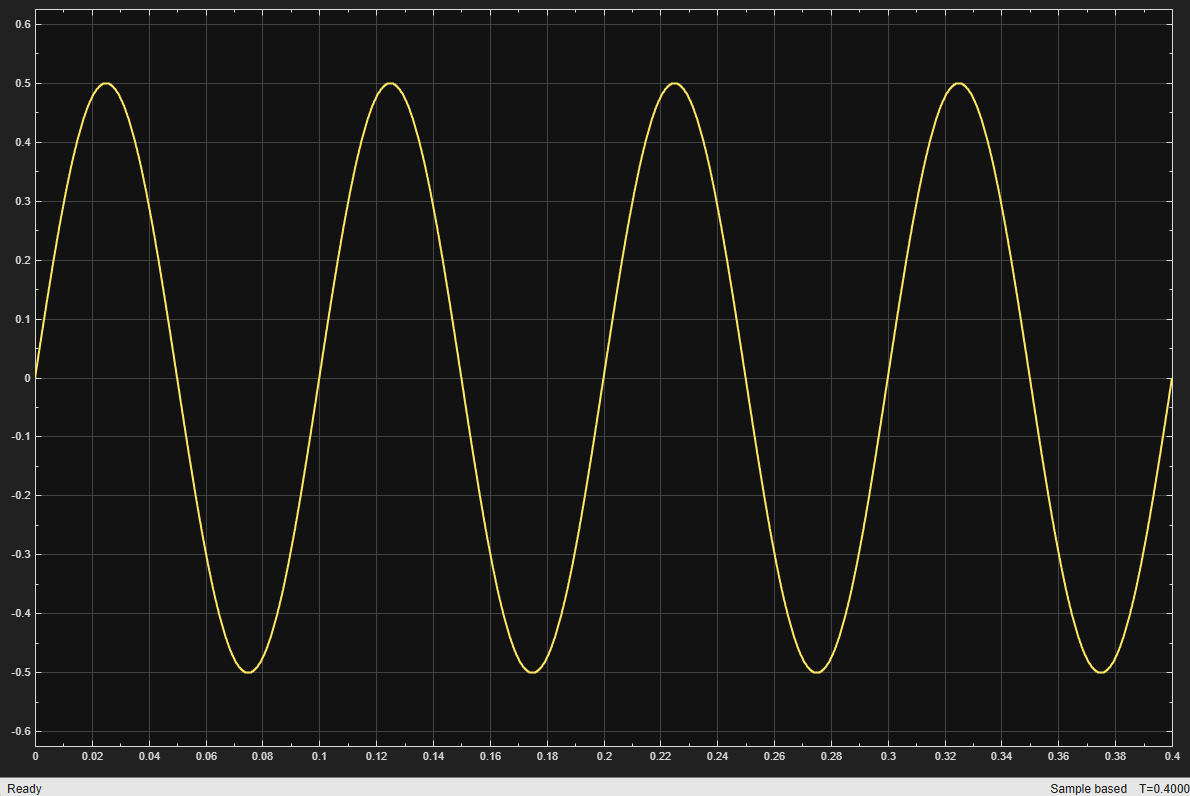
\includegraphics[width=\linewidth]{sine-scope.png}
        \caption{Time domain.}
    \end{subfigure}
    \hfill
    \begin{subfigure}[b]{0.48\textwidth}
        \centering
        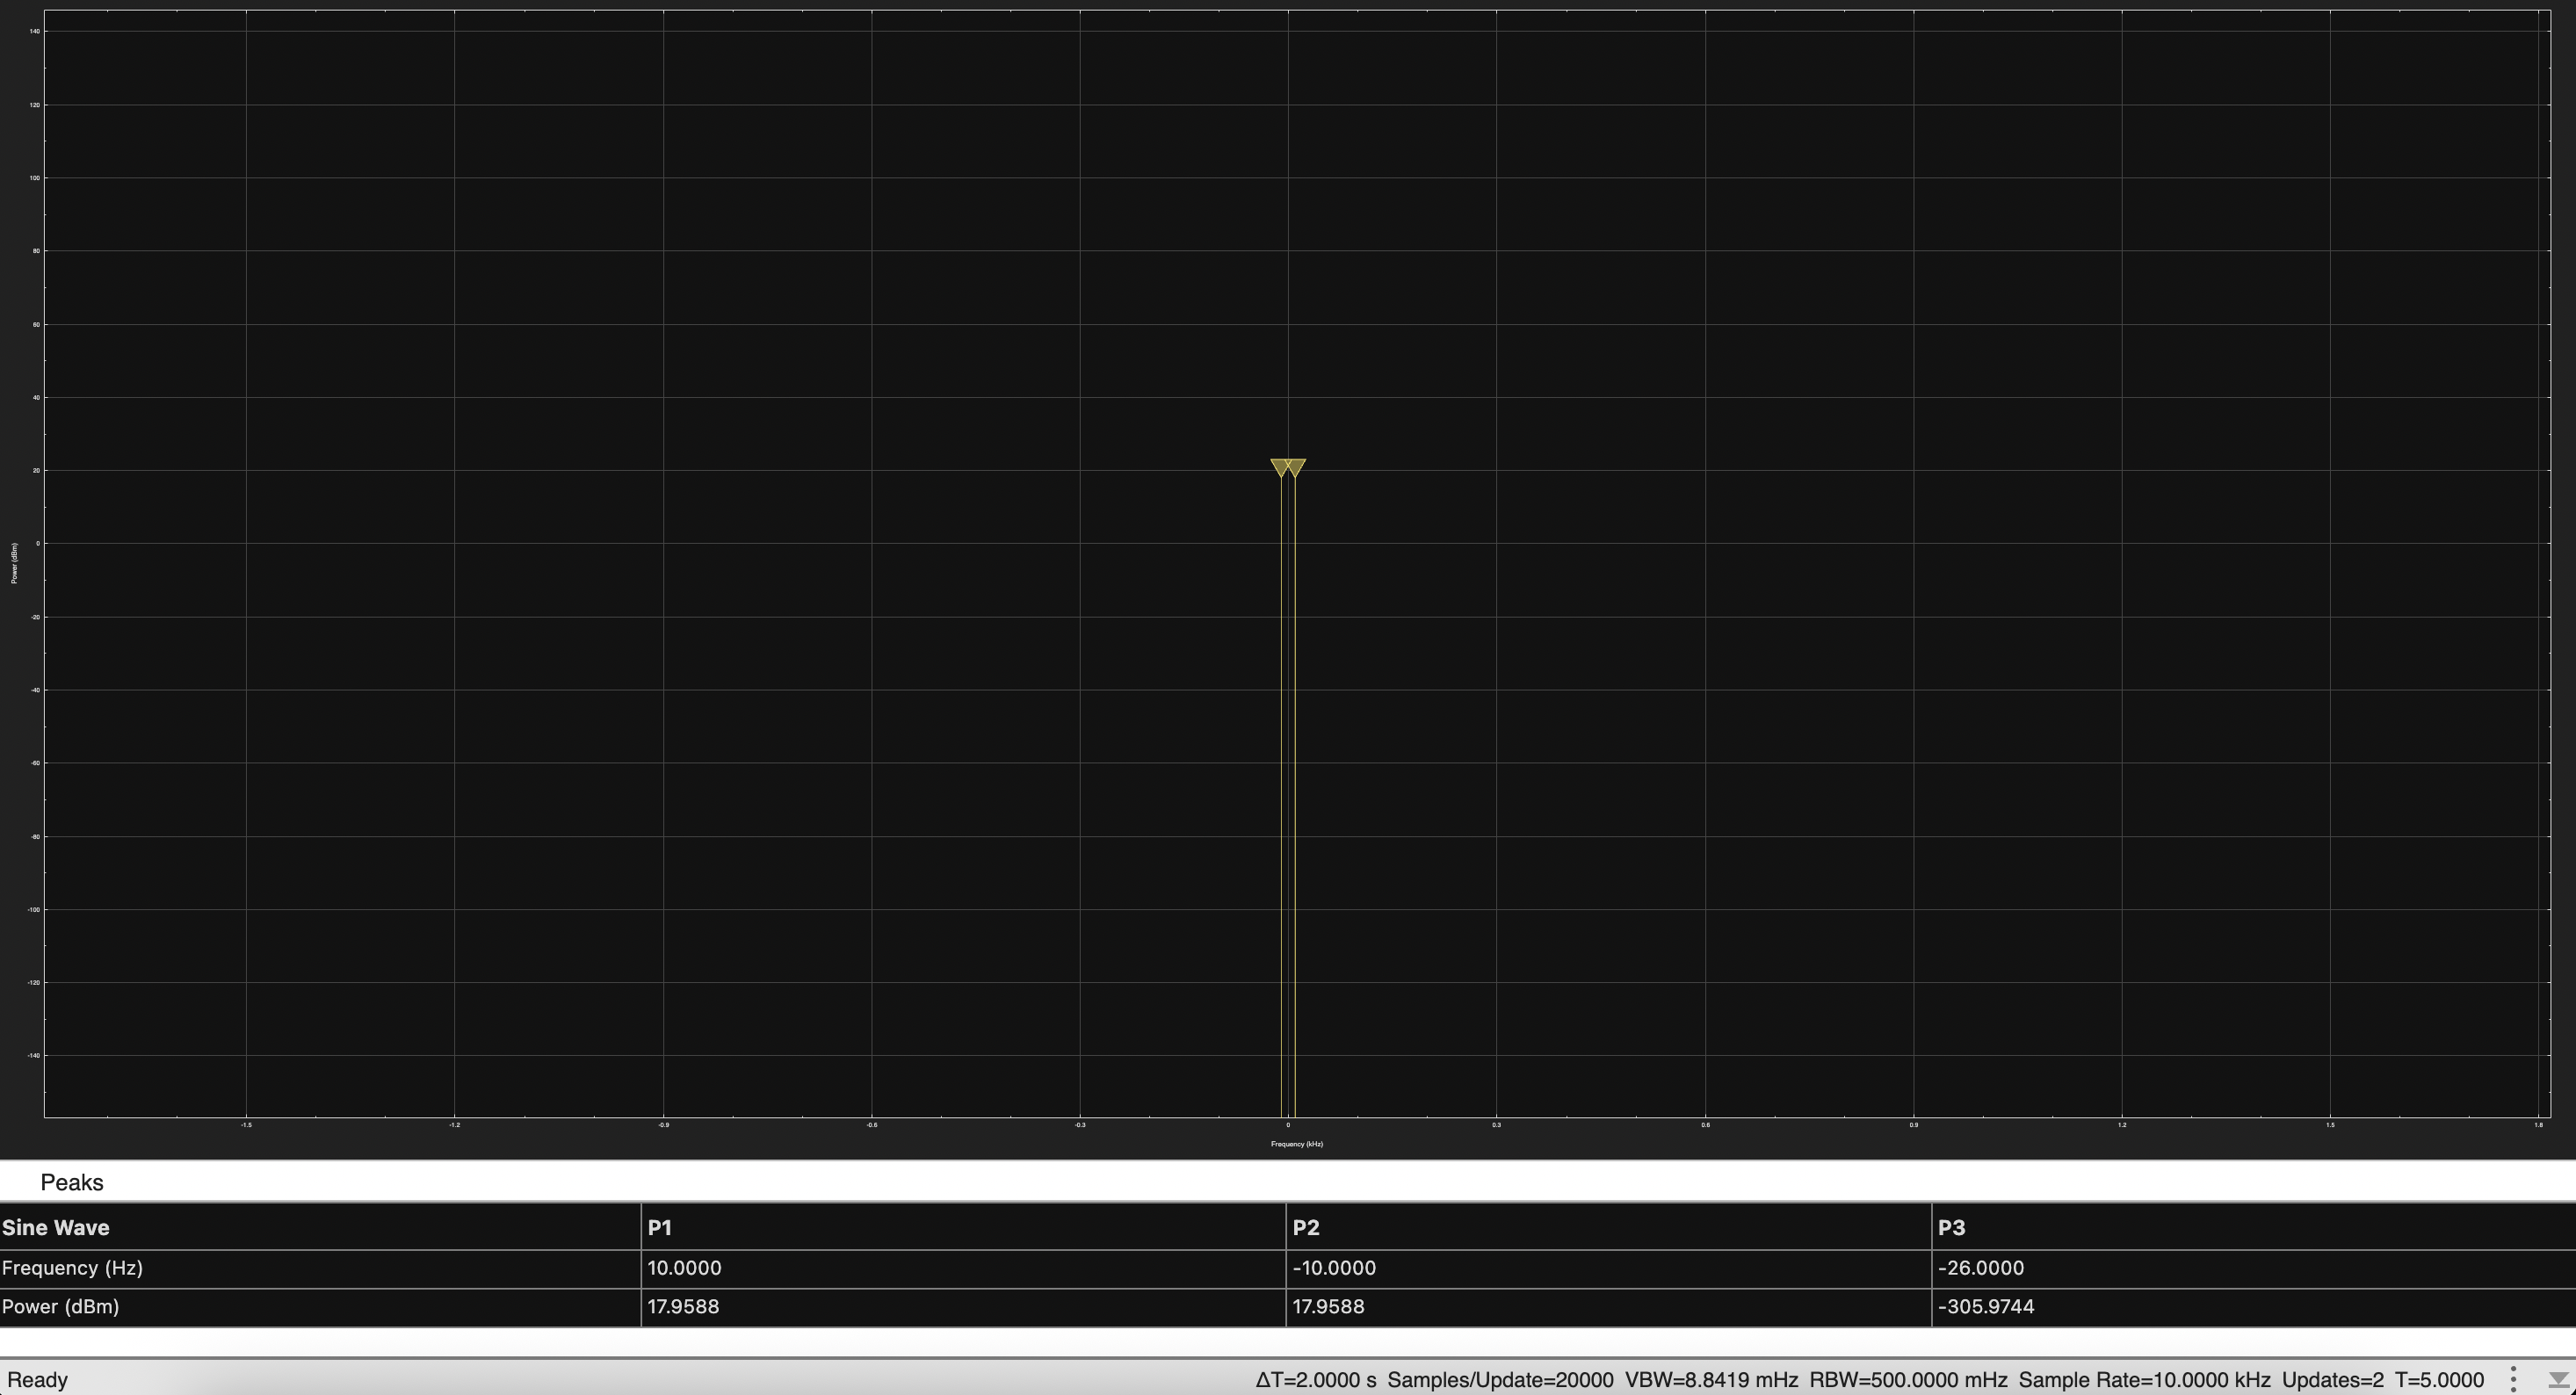
\includegraphics[width=\linewidth]{q1_spectrum.png}
        \caption{Spectrum.}
    \end{subfigure}
    \caption{Sine wave (amplitude 0.5, T = 0.1s, f = 10\,Hz) shown over four periods, with its spectrum. An ideal sine wave does not have harmonics.
    but we can observe the power of 17.9588 dBm at 10\,Hz matches expected amplitude of 0.5.}
    \label{fig:sine}
\end{figure}

\subsection*{Question 2}

% Same analysis for the triangular wave.

\begin{figure}[H]
    \centering
    \begin{subfigure}[b]{0.48\textwidth}
        \centering
        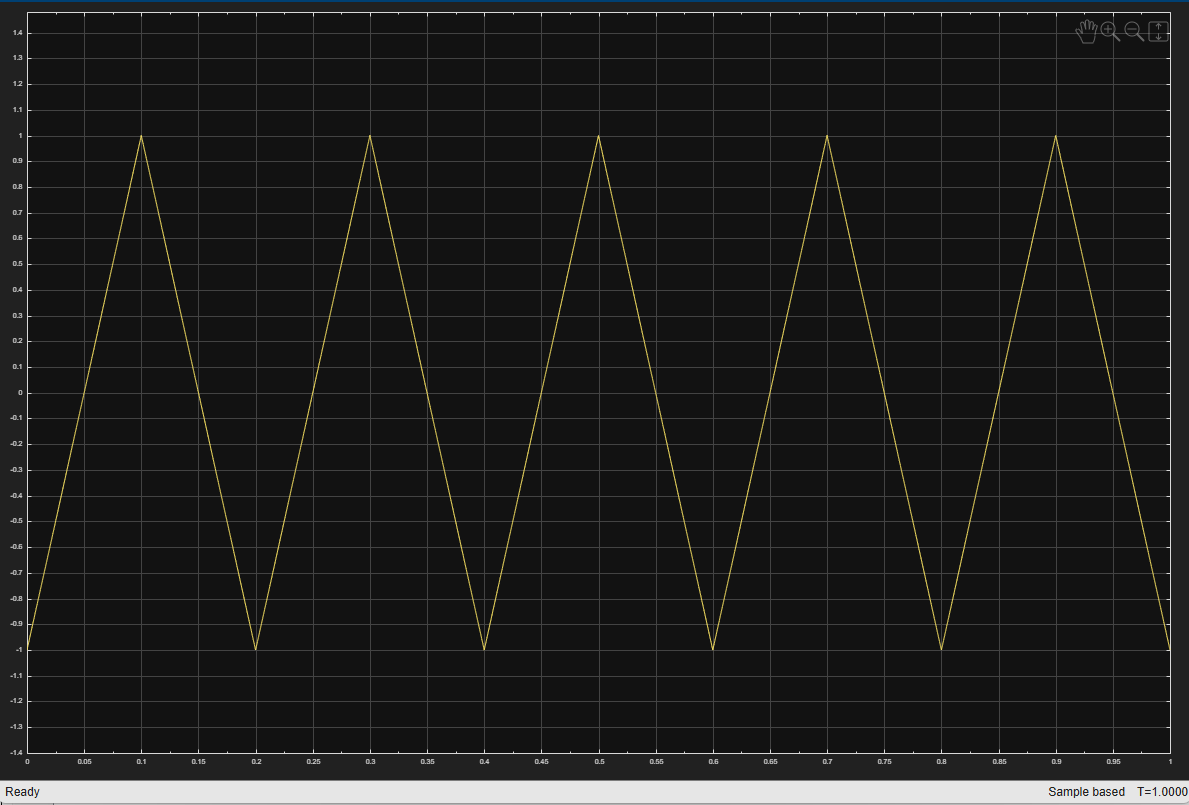
\includegraphics[width=\linewidth]{triangle-scope.png}
        \caption{Time domain.}
    \end{subfigure}
    \hfill
    \begin{subfigure}[b]{0.48\textwidth}
        \centering
        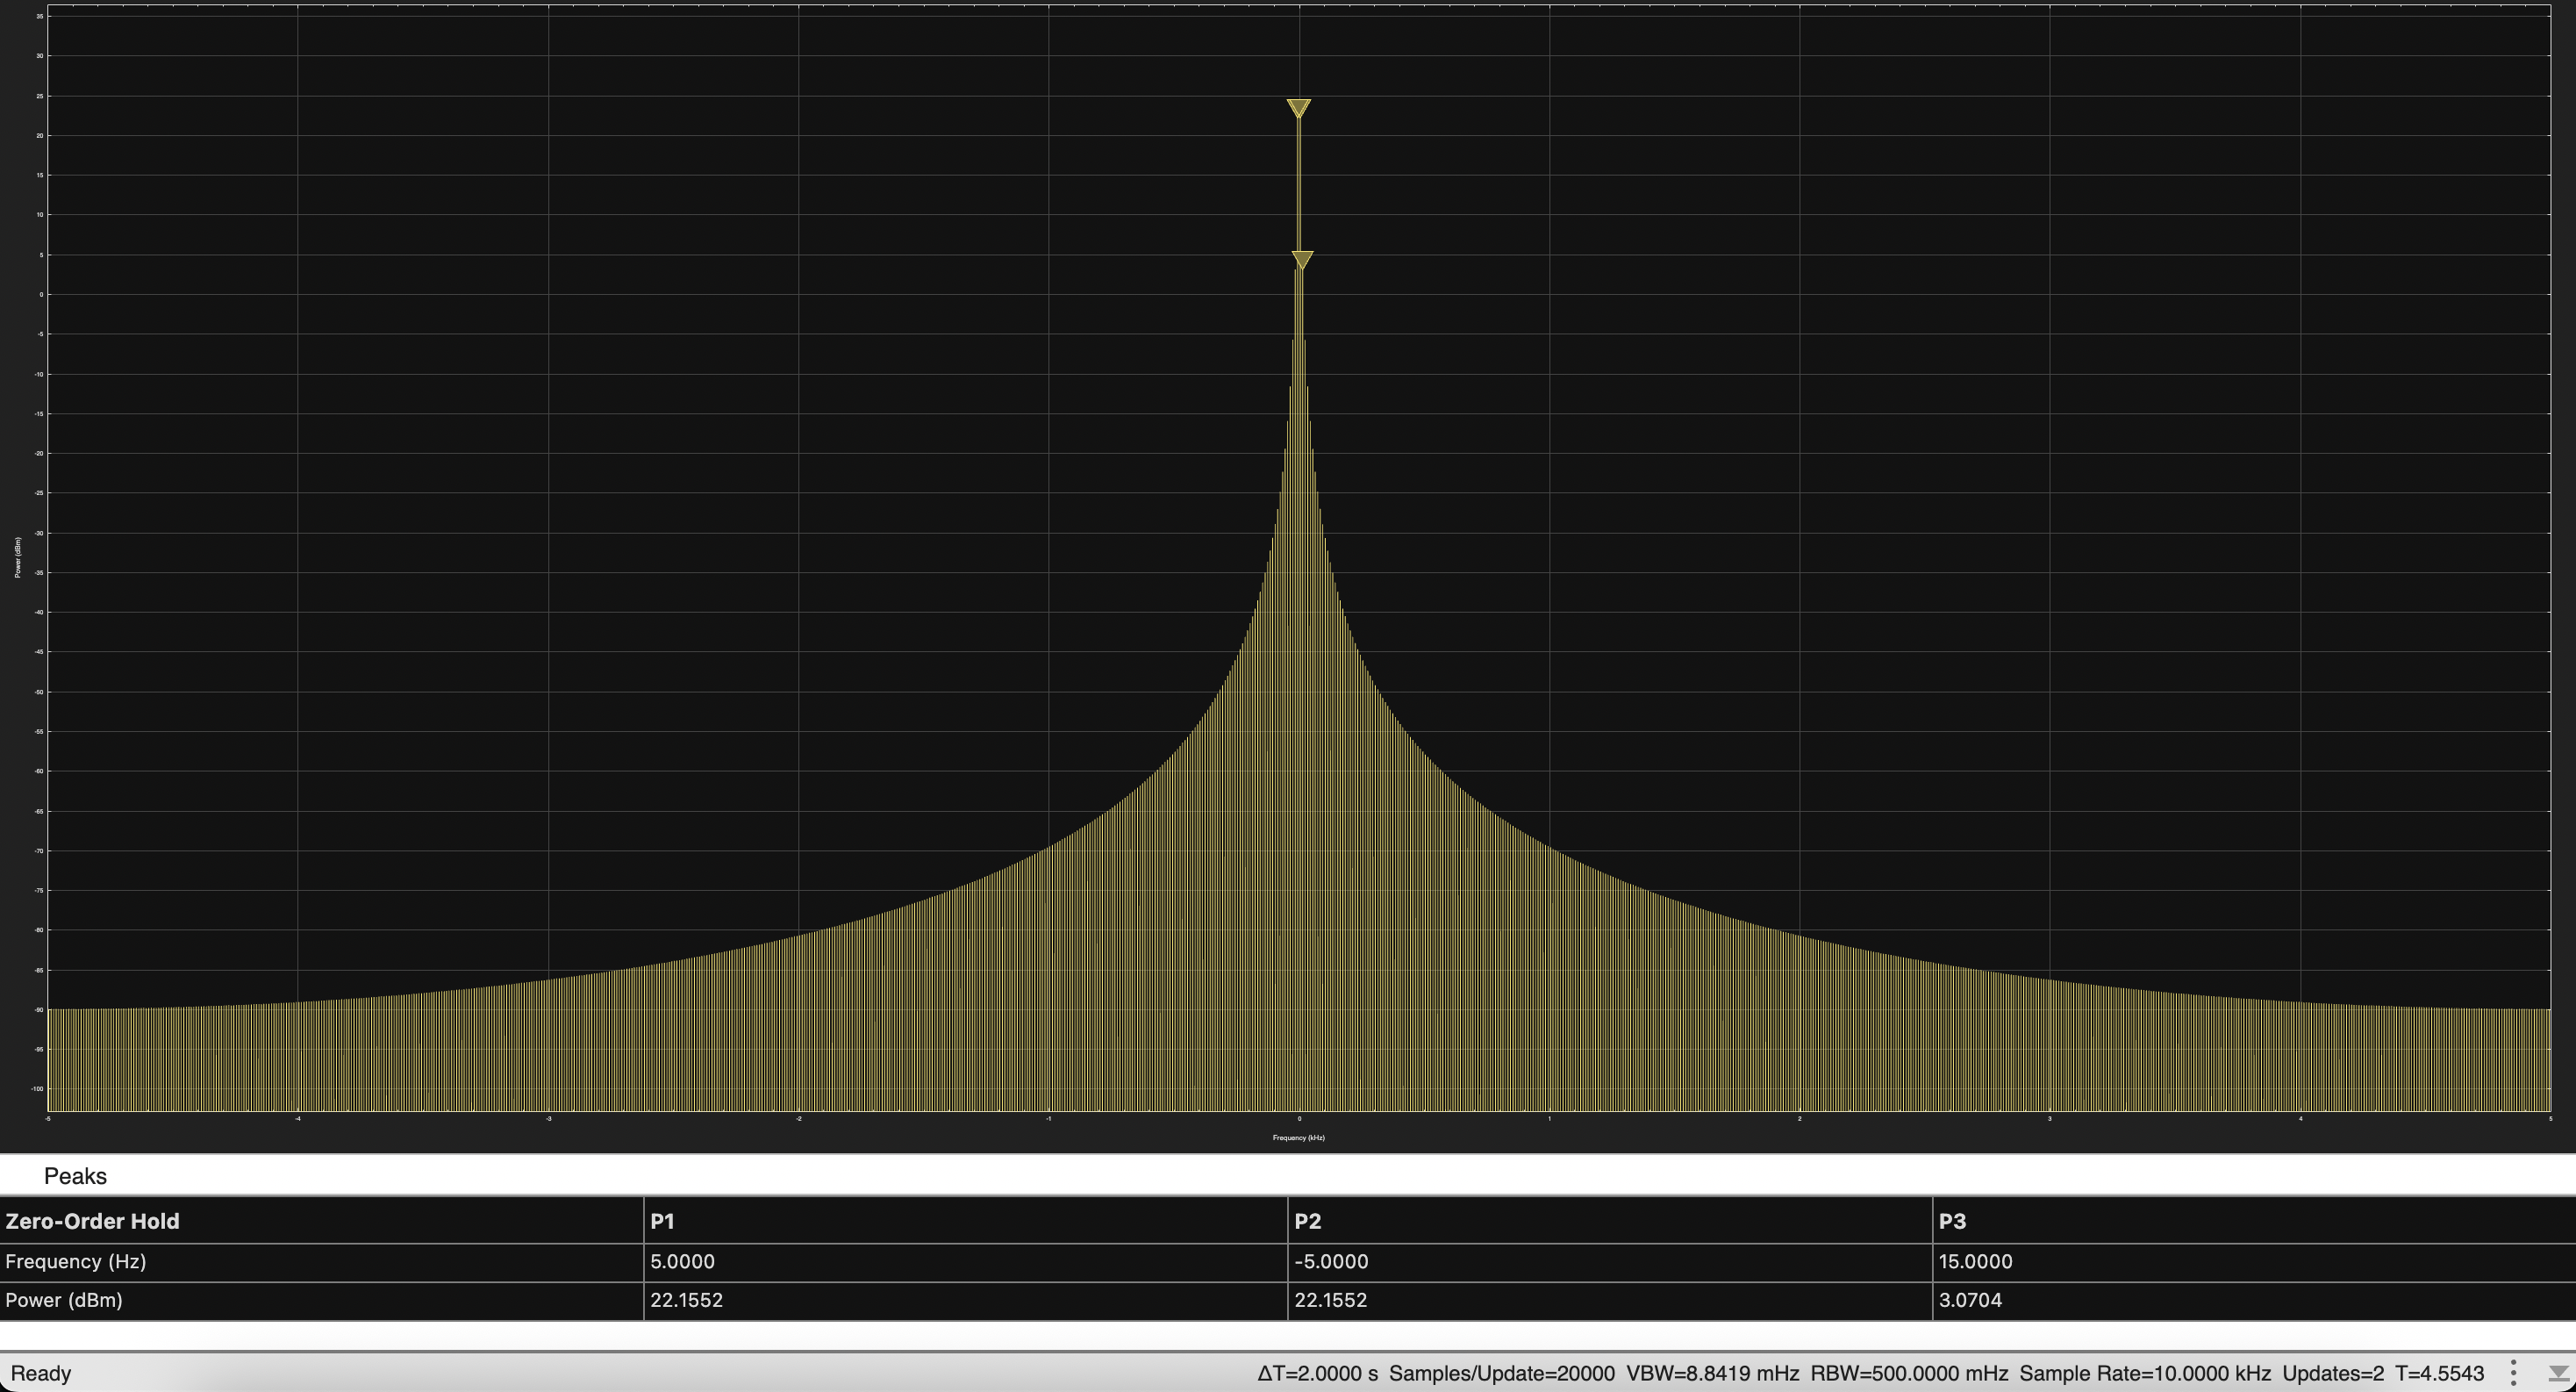
\includegraphics[width=\linewidth]{q2_spectrum.png}
        \caption{Spectrum.}
    \end{subfigure}
    \caption{Triangular wave: amplitude 1, $T=0.2$\,s, $f_0=5$\,Hz. Only odd harmonics (5, 15, 25, $\ldots$\,Hz) occur, with amplitudes decreasing as $1/n^2$.}
    \label{fig:triangle}
\end{figure}

\subsection*{Question 3}

% 50\% duty cycle square wave.

\begin{figure}[H]
    \centering
    \begin{subfigure}[b]{0.48\textwidth}
        \centering
        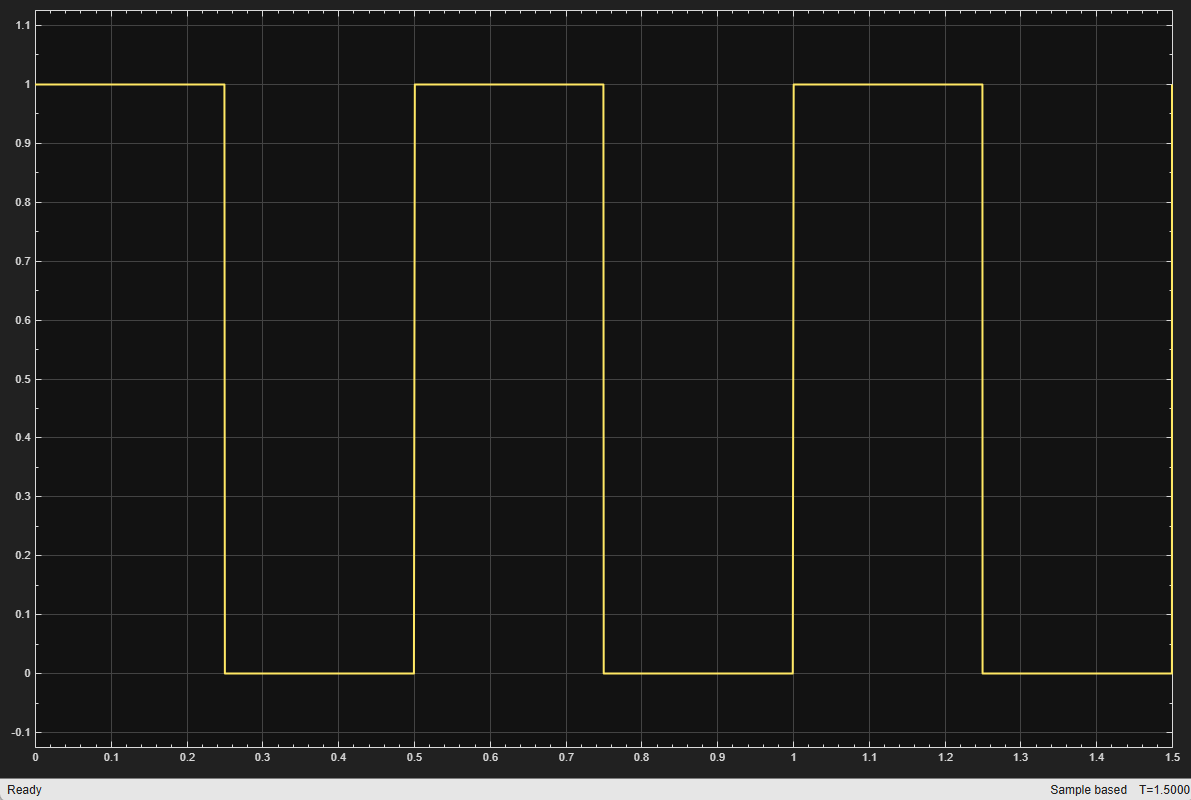
\includegraphics[width=\linewidth]{pulse-scope-50.png}
        \caption{Time domain.}
    \end{subfigure}
    \hfill
    \begin{subfigure}[b]{0.48\textwidth}
        \centering
        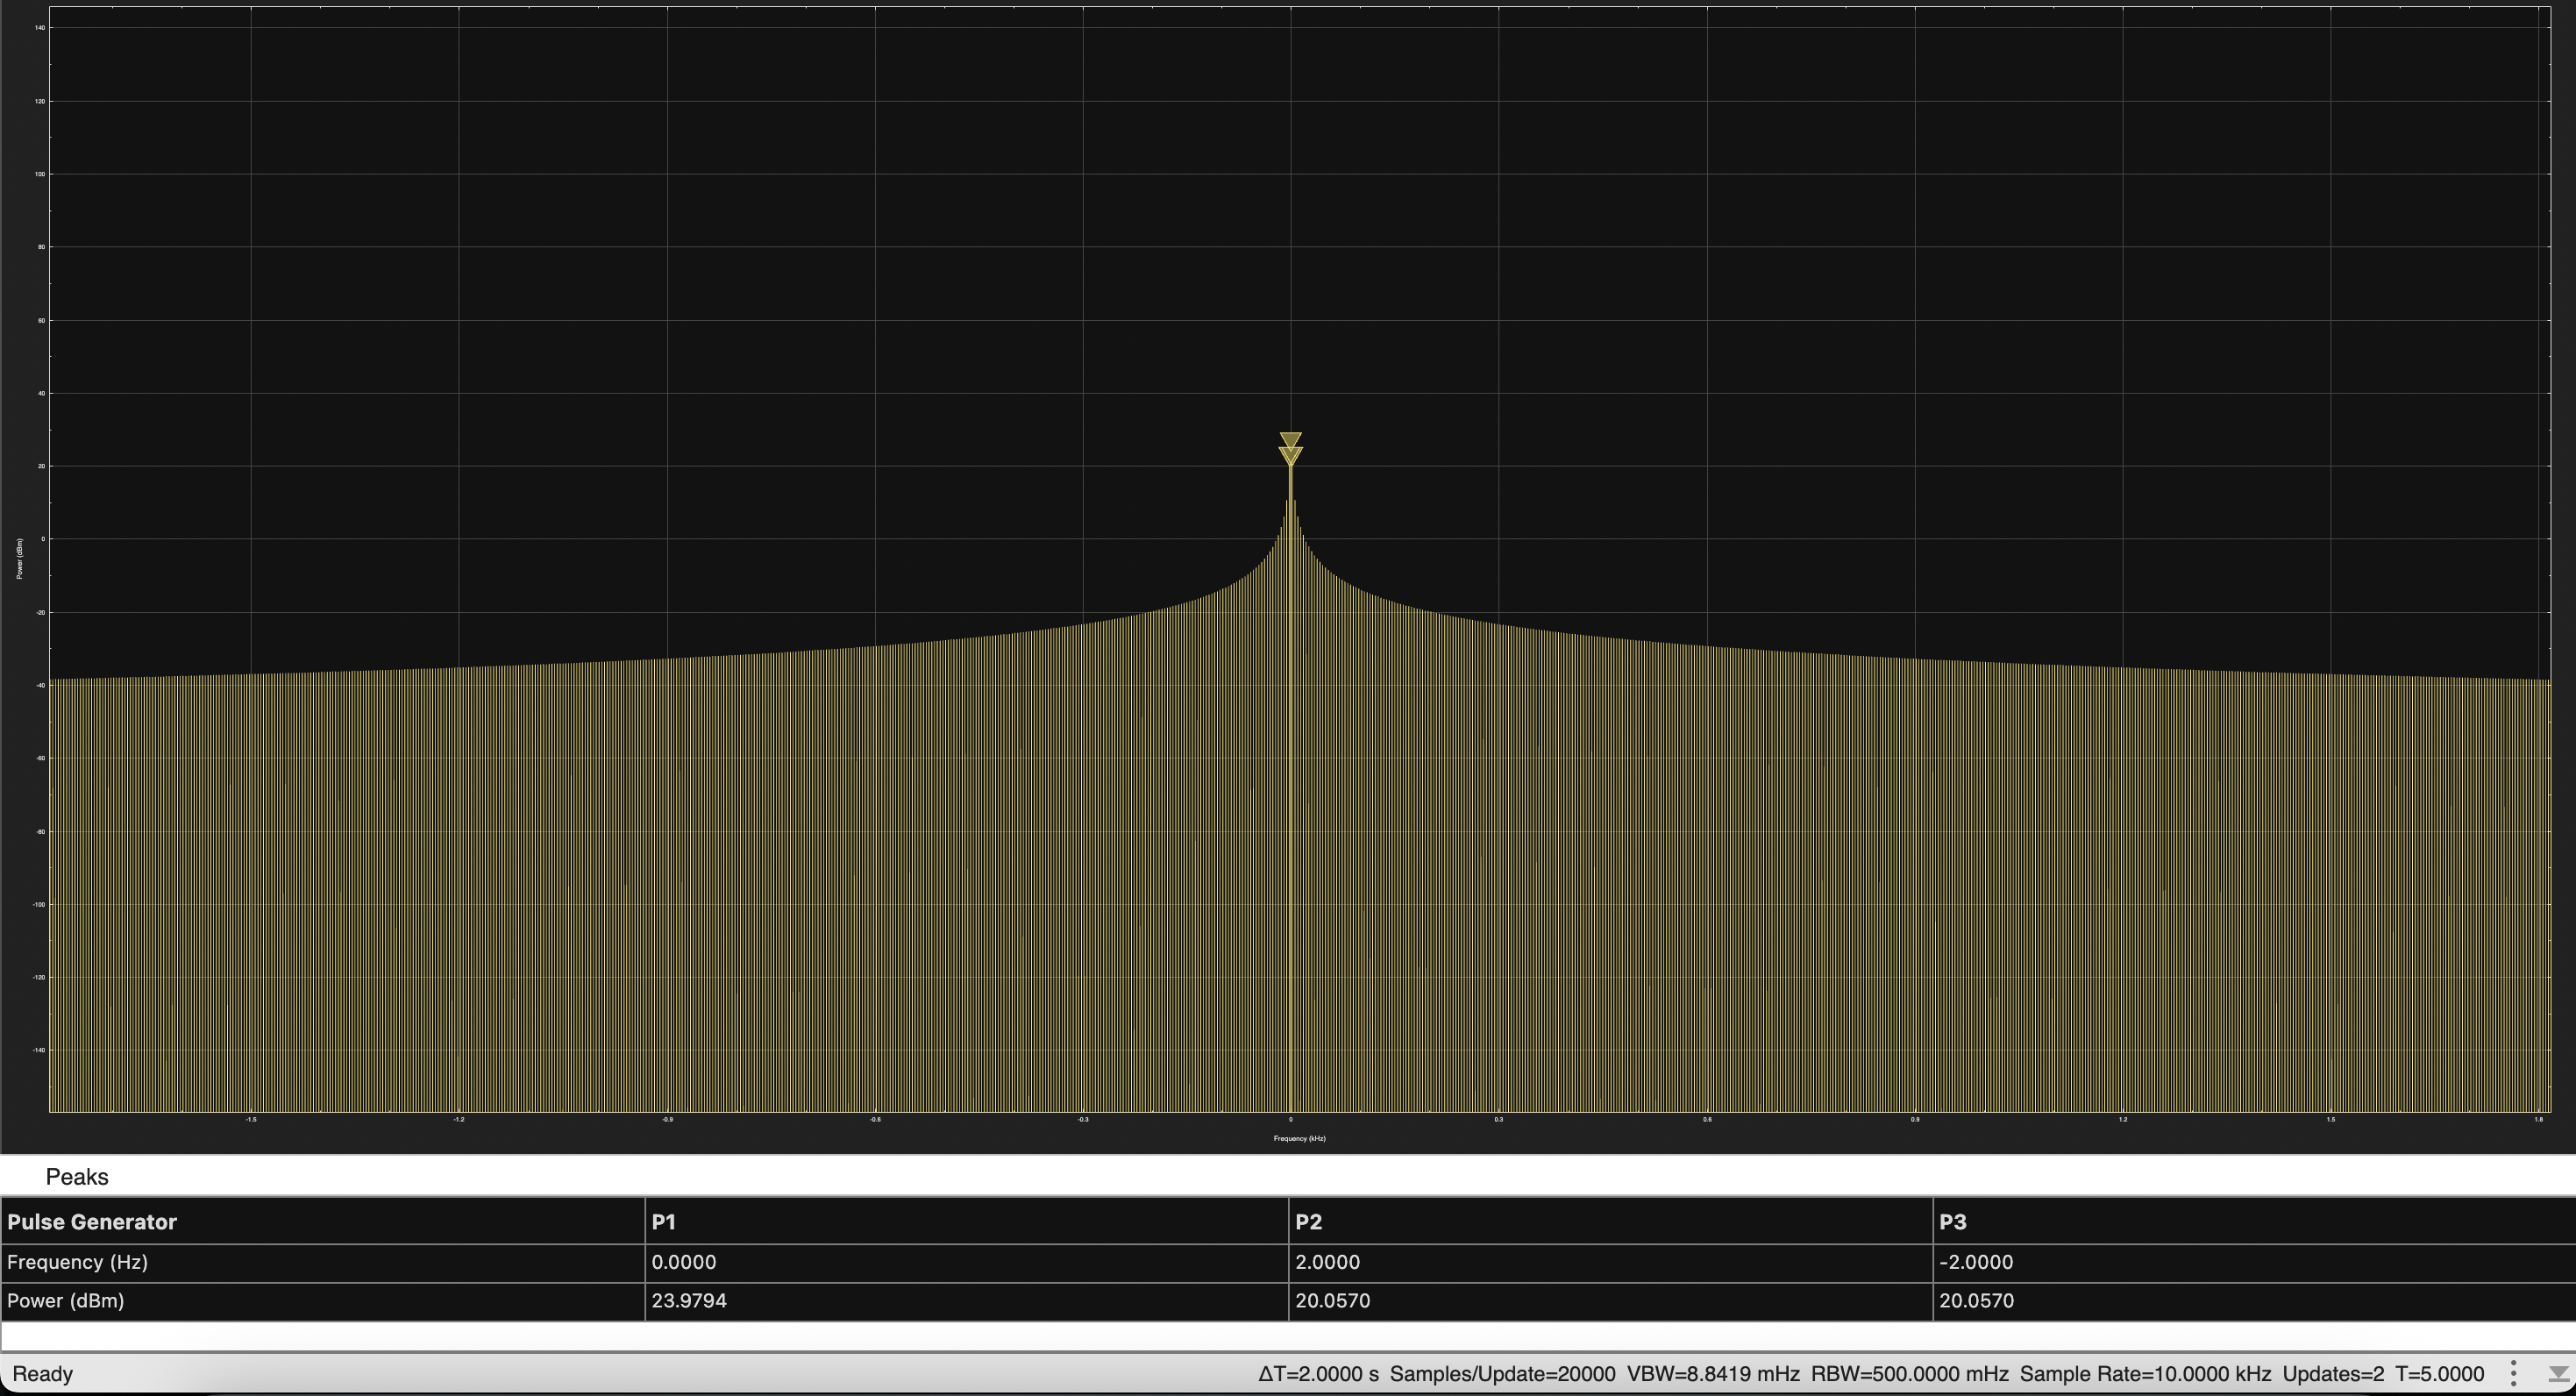
\includegraphics[width=\linewidth]{q3_spectrum.png}
        \caption{Spectrum.}
    \end{subfigure}
    \caption{50\% duty-cycle pulse train (0 to 1.5): $T=0.5$\,s, $f_0=2$\,Hz, DC level 0.5. Only odd harmonics (2, 6, 10, $\ldots$\,Hz) occur, with amplitudes decreasing as $1/n$.}
    \label{fig:pulse50}
\end{figure}

\subsection*{Question 4}

% 20\% duty cycle square wave -- note which harmonics are missing and why.

\begin{figure}[H]
    \centering
    \begin{subfigure}[b]{0.48\textwidth}
        \centering
        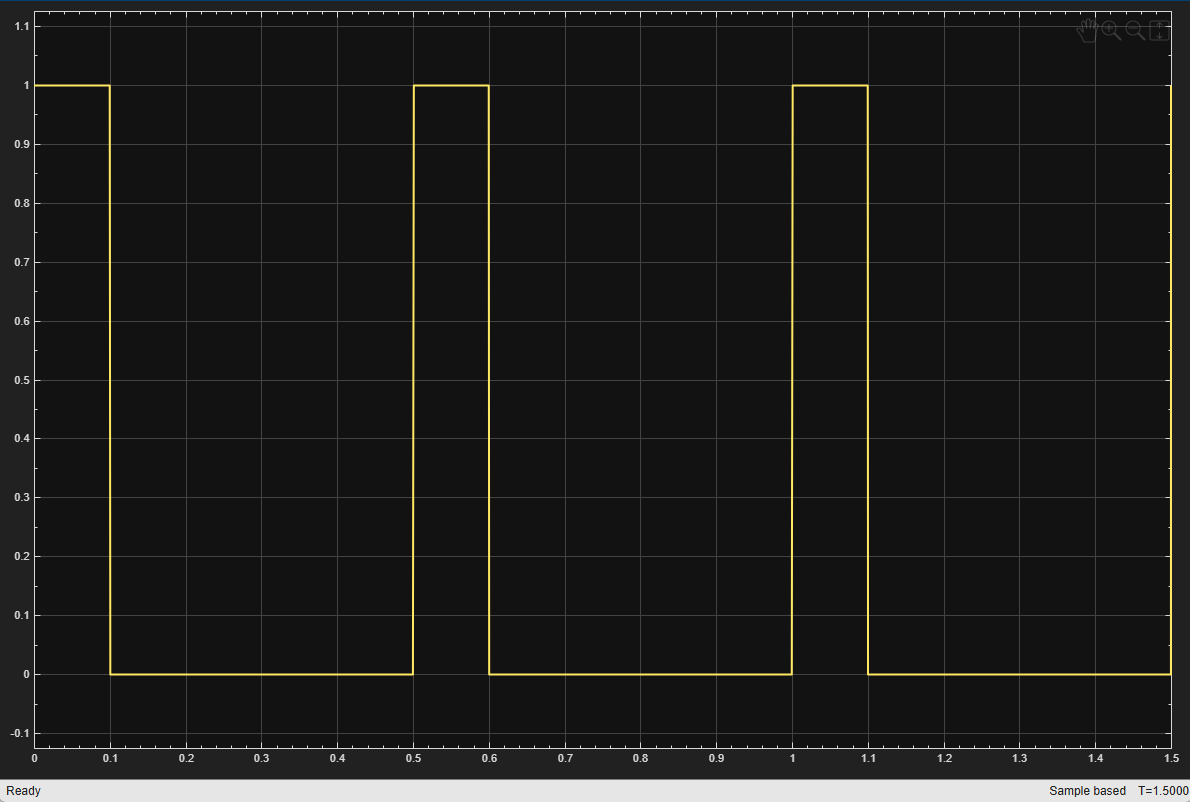
\includegraphics[width=\linewidth]{pulse-scope-20.png}
        \caption{Time domain.}
    \end{subfigure}
    \hfill
    \begin{subfigure}[b]{0.48\textwidth}
        \centering
        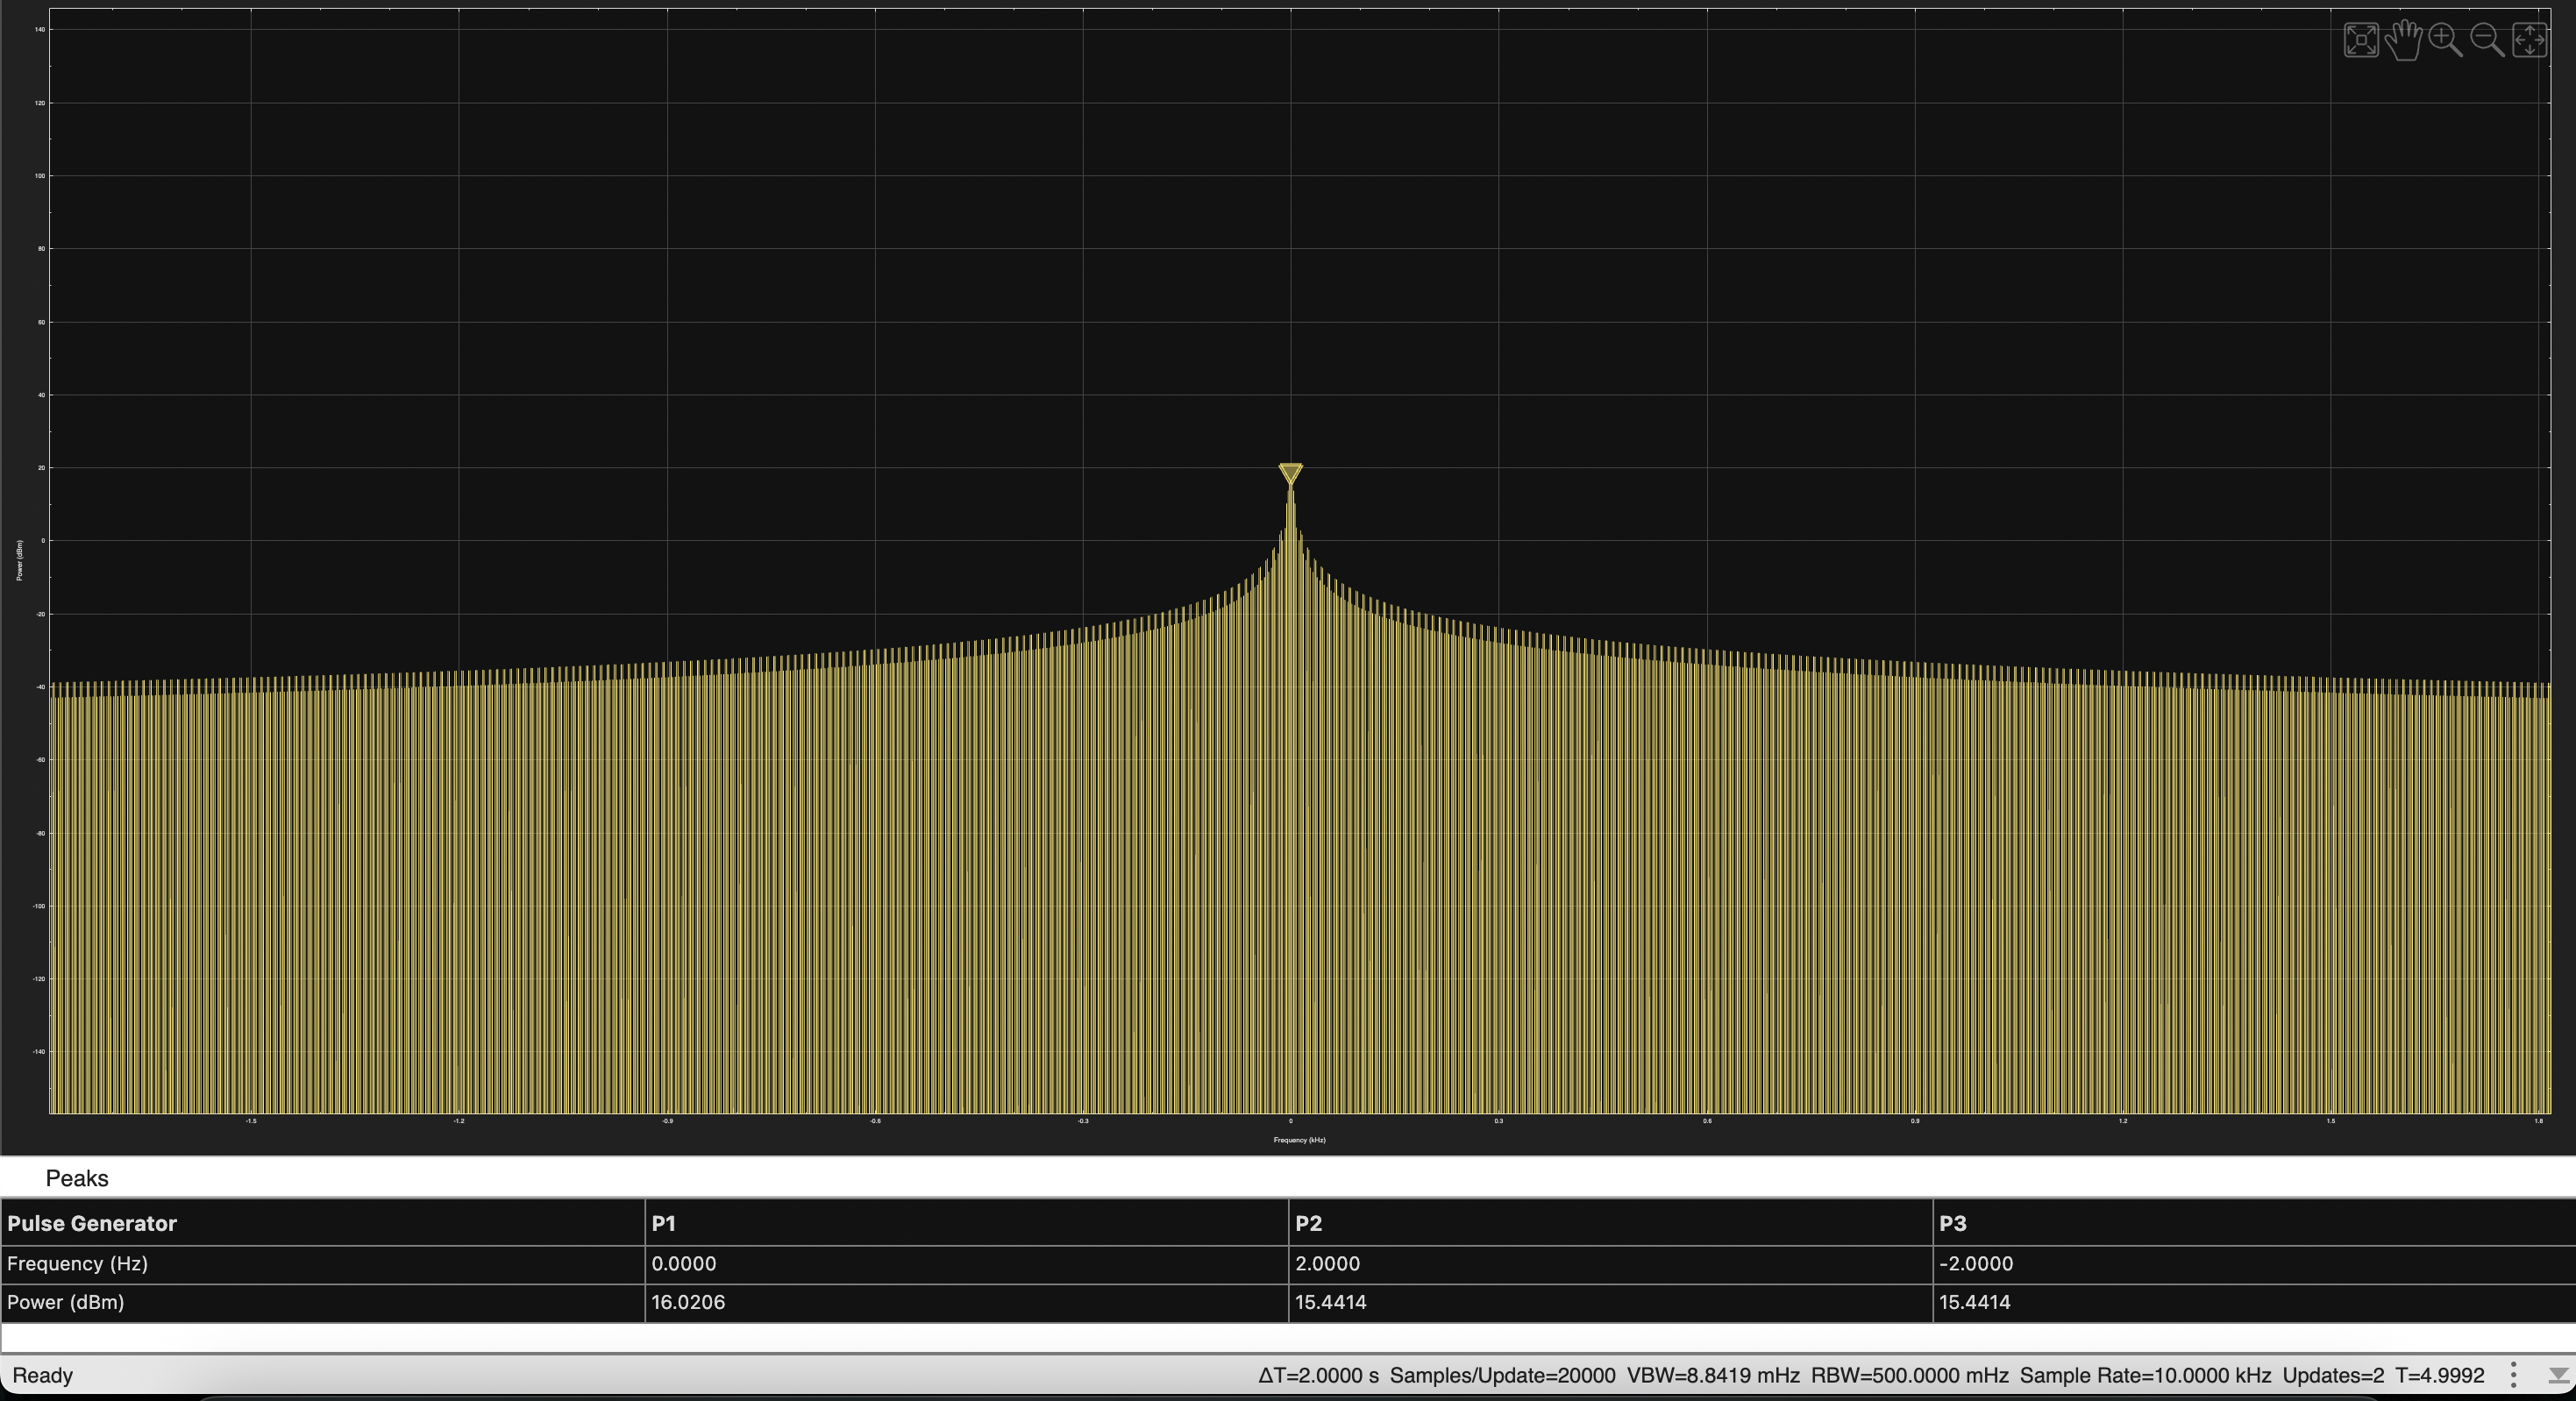
\includegraphics[width=\linewidth]{q4_spectrum.png}
        \caption{Spectrum.}
    \end{subfigure}
    \caption{20\% duty-cycle pulse train (0 to 1.5): $T=0.5$\,s, $f_0=2$\,Hz, DC level 0.2. Harmonics occur at $2n$\,Hz, except every fifth harmonic (10, 20, 30, $\ldots$\,Hz), which vanishes.}
    \label{fig:pulse20}
\end{figure}

\subsection*{Question 5}

% Sum of three sine waves: identify each component and the period of the sum.

\begin{figure}[H]
    \centering
    \begin{subfigure}[b]{0.48\textwidth}
        \centering
        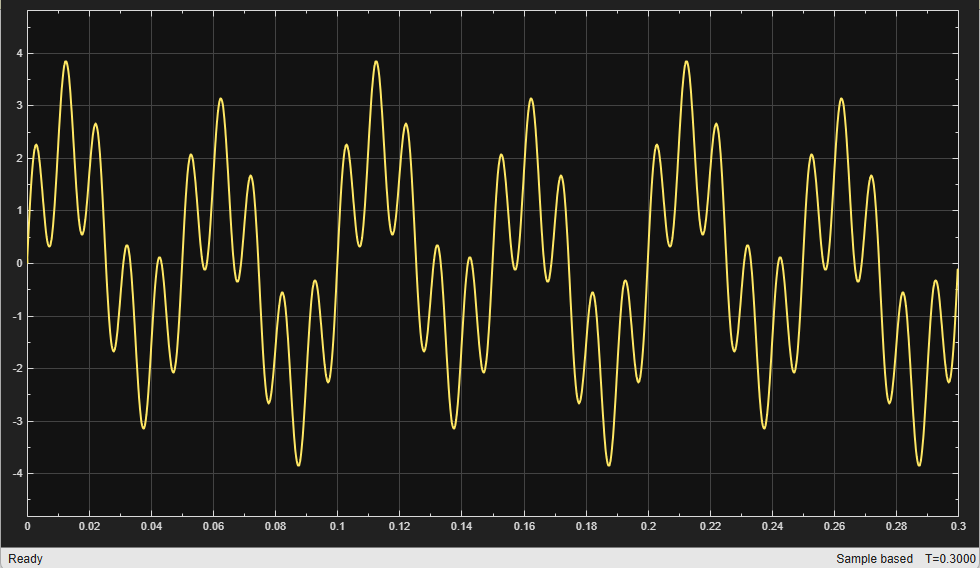
\includegraphics[width=\linewidth]{sum-sine-scope.png}
        \caption{Time domain.}
    \end{subfigure}
    \hfill
    \begin{subfigure}[b]{0.48\textwidth}
        \centering
        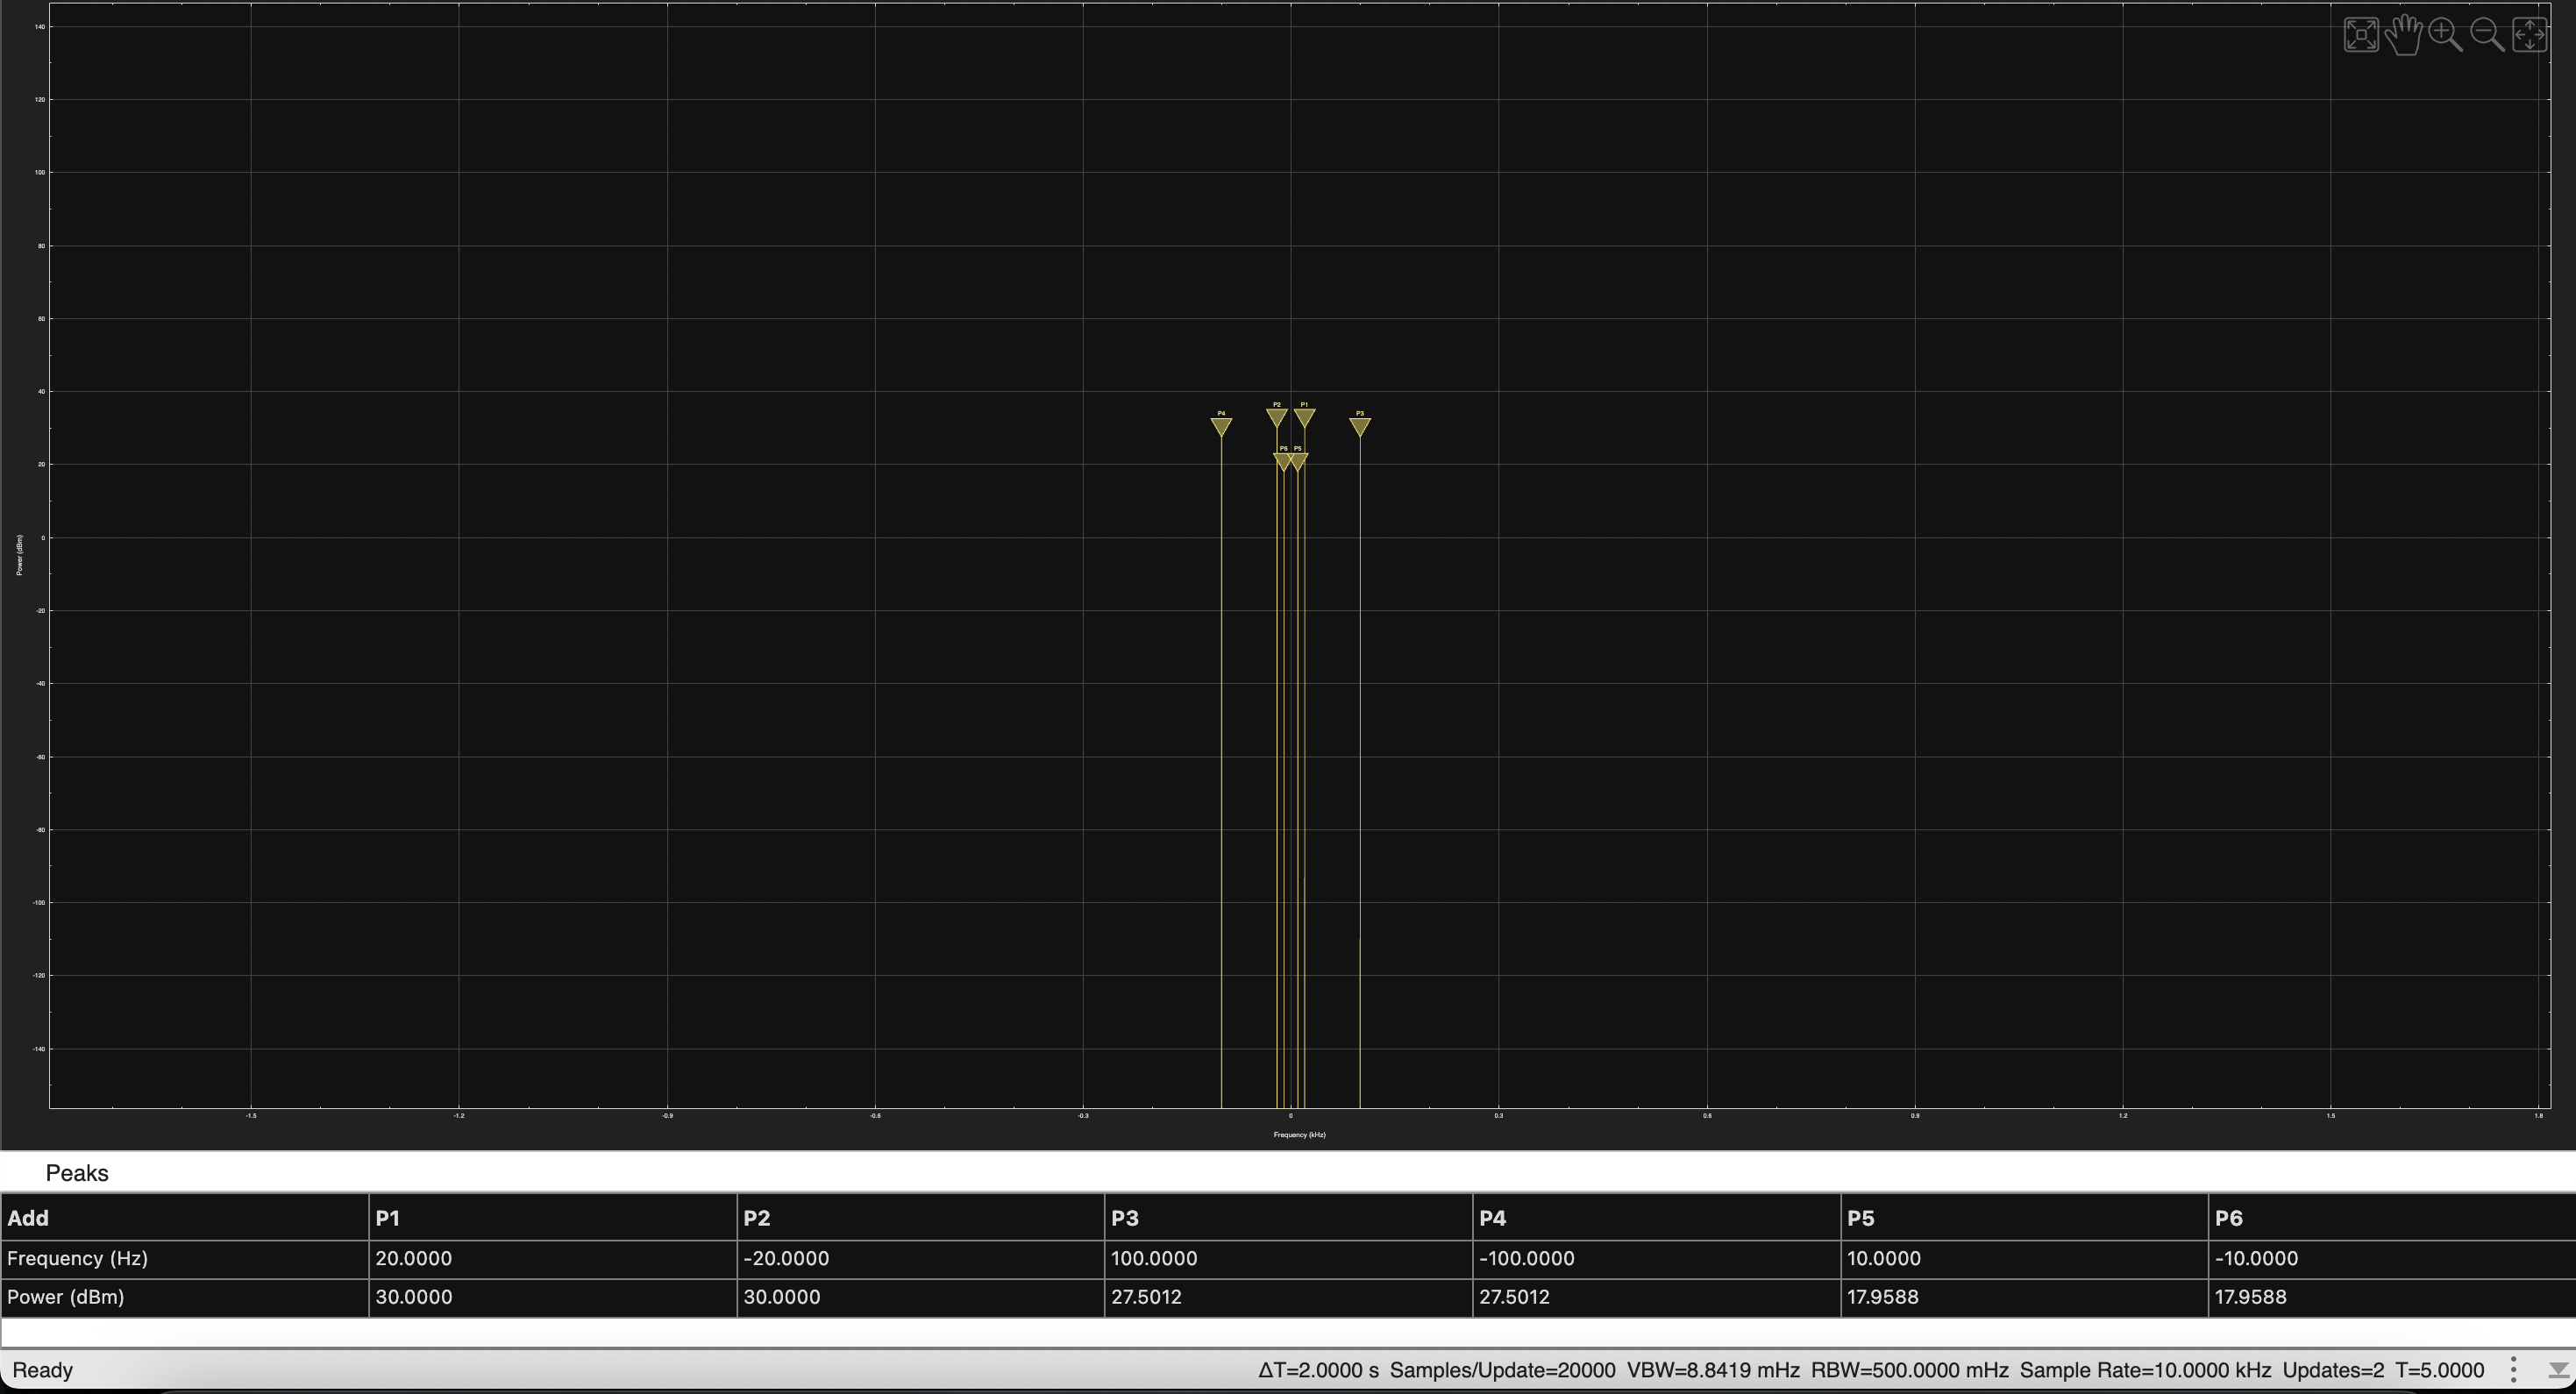
\includegraphics[width=\linewidth]{q5_spectrum.png}
        \caption{Spectrum.}
    \end{subfigure}
    \caption{Sum of sine waves at 10, 20 and 100\,Hz with amplitudes 0.5, 2 and 1.5, respectively. The sum has $T=0.1$\,s and $f_0=10$\,Hz; only the fundamental, second and tenth harmonics are present.}
    \label{fig:sumsine}
\end{figure}

\subsection*{Question 6}

% Comment on the periodicity of the step-gated sine waves.

\begin{figure}[H]
    \centering
    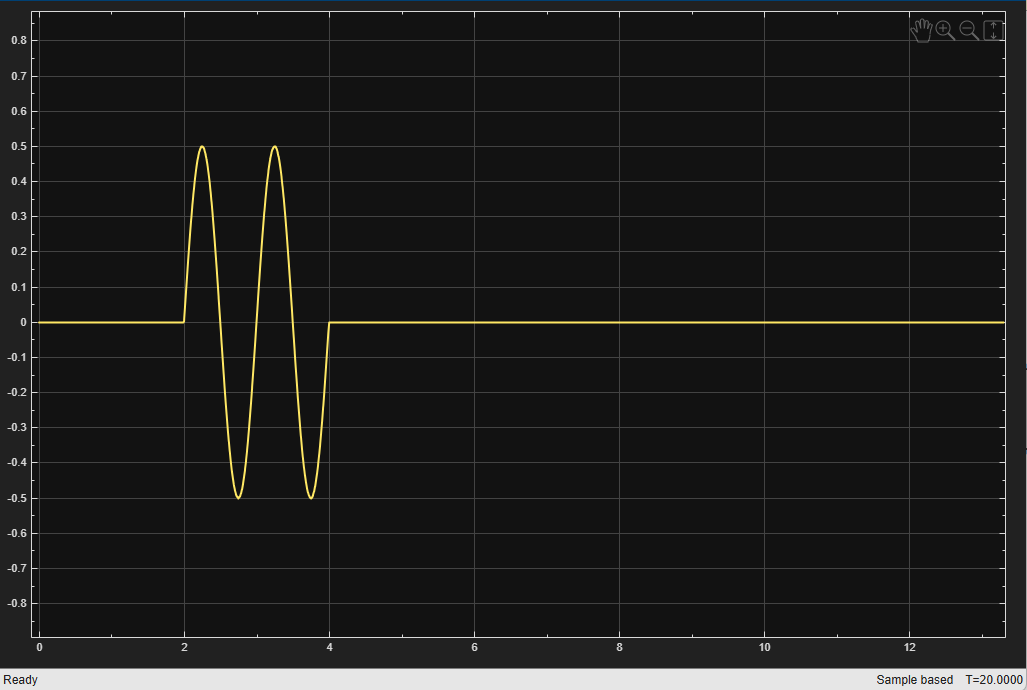
\includegraphics[width=0.55\textwidth]{product-sine-step-scope.png}
    \caption{Difference of two step-gated sine waves (steps at $t = 2$\,s and $t = 4$\,s) observed on the Scope. Here we observe no overall periodicity
    in the resulting signal due to it being "turned off" at 4\,s.}
    \label{fig:productstep}
\end{figure}

\subsection*{Question 7}

% Bandwidth and power spectral density of the thermal noise.

\begin{figure}[H]
    \centering
    \begin{subfigure}[b]{0.48\textwidth}
        \centering
        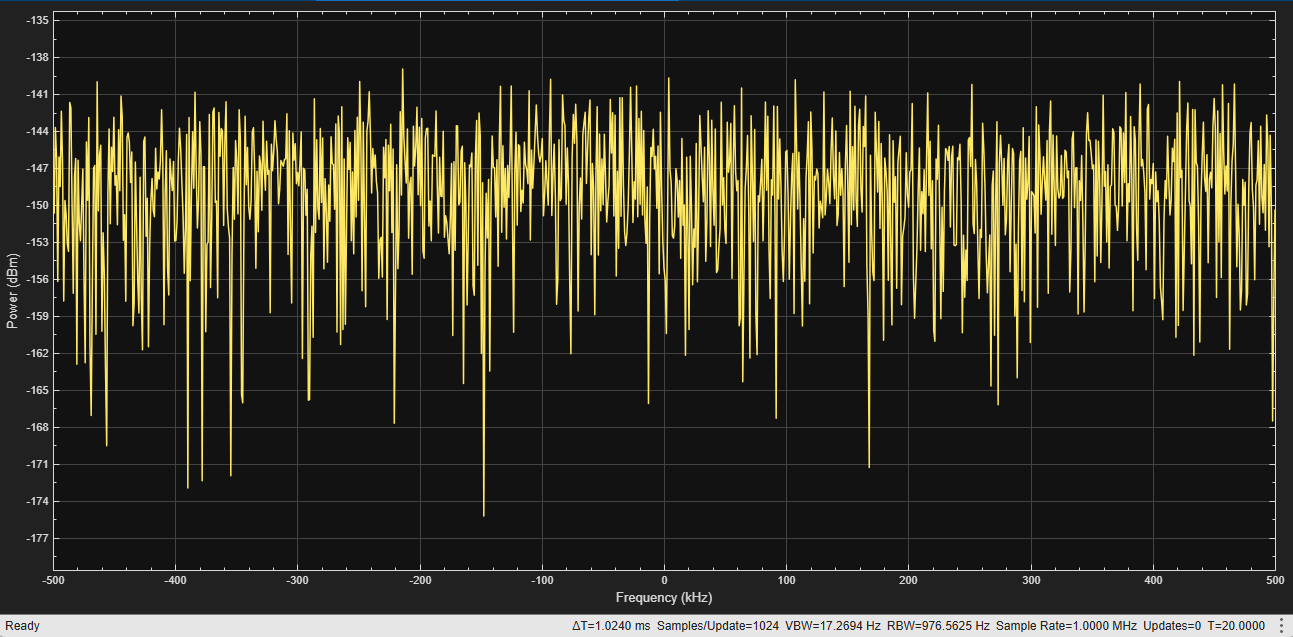
\includegraphics[width=\textwidth]{thermal-noise.png}
        \caption{Single trace.}
        \label{fig:thermal-raw}
    \end{subfigure}
    \hfill
    \begin{subfigure}[b]{0.48\textwidth}
        \centering
        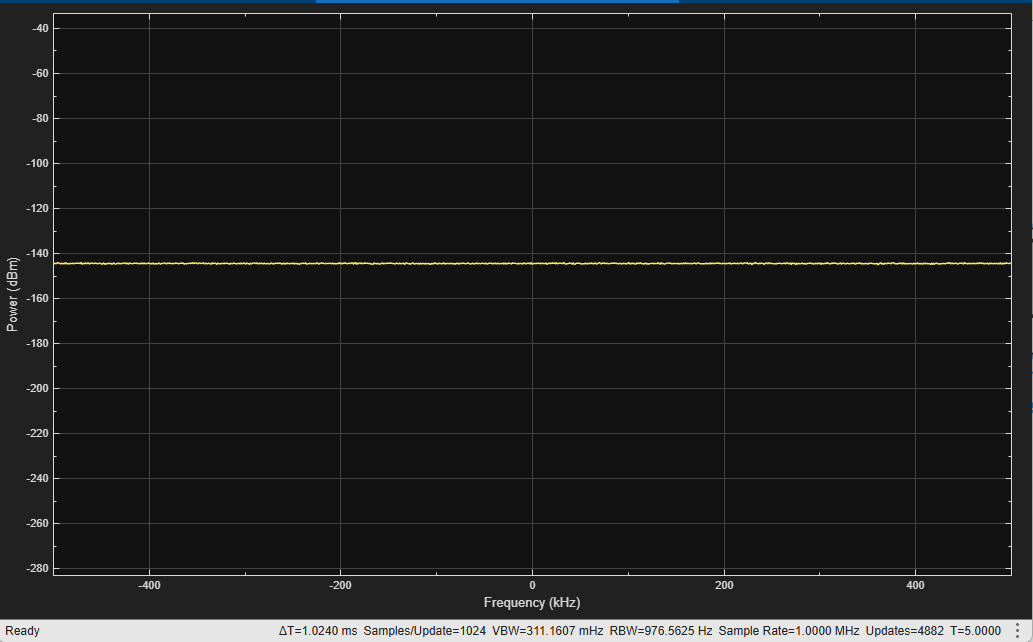
\includegraphics[width=\textwidth]{thermal-noise-smooth.png}
        \caption{With trace averaging.}
        \label{fig:thermal-smooth}
    \end{subfigure}
    \caption{Thermal noise at 290\,K occupies the full displayed range from $-500$ to $+500$\,kHz, a two-sided observed bandwidth of 1\,MHz set by the sampling rate.}
    \label{fig:thermal}
\end{figure}

\begin{figure}[H]
    \centering
    \begin{subfigure}[b]{0.48\textwidth}
        \centering
        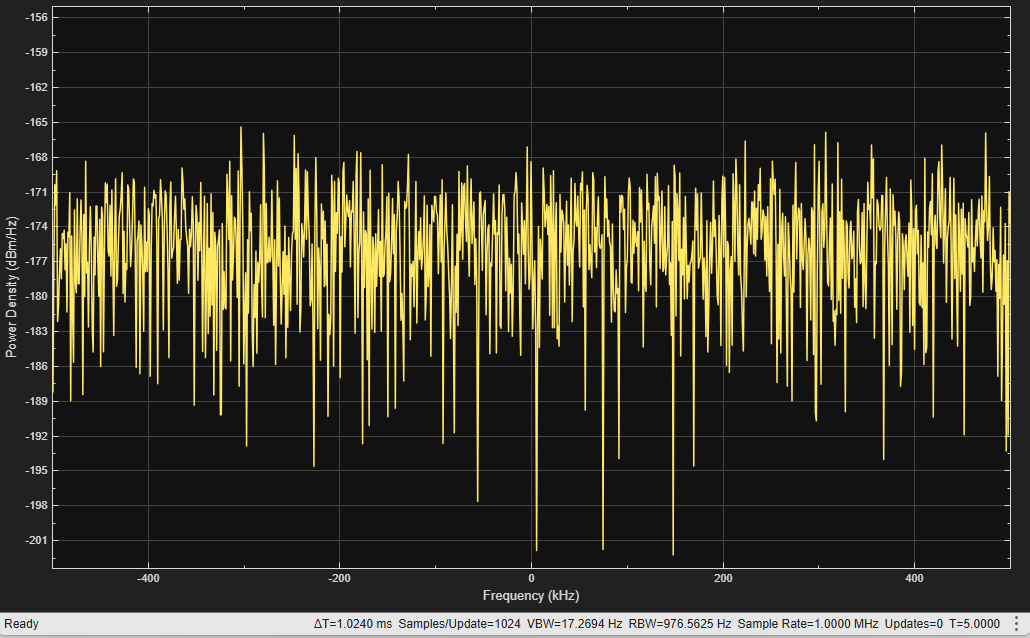
\includegraphics[width=\textwidth]{thermal-noise-density.png}
        \caption{Single trace.}
        \label{fig:thermal-density-raw}
    \end{subfigure}
    \hfill
    \begin{subfigure}[b]{0.48\textwidth}
        \centering
        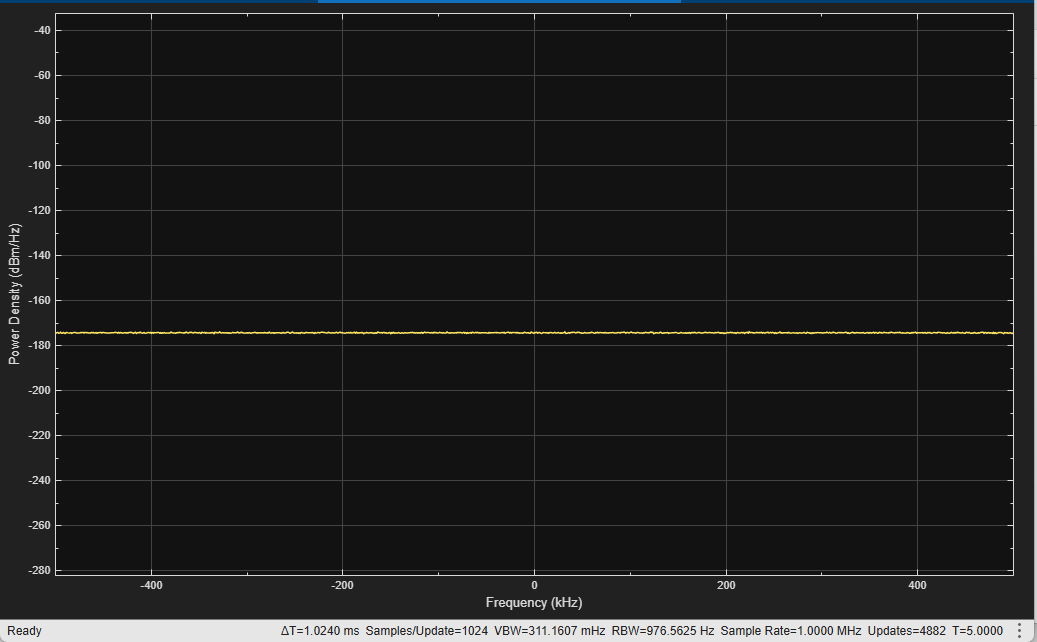
\includegraphics[width=\textwidth]{thermal-noise-density-smooth.png}
        \caption{With trace averaging.}
        \label{fig:thermal-density-smooth}
    \end{subfigure}
    \caption{The thermal-noise PSD is approximately flat at $-174$\,dBm/Hz, consistent with $kT$ at 290\,K. Trace averaging reduces fluctuations in the estimate, revealing the flat noise density.}
    \label{fig:thermal-density}
\end{figure}

\subsection*{Question 8}

% Relate the peak of the autocorrelation at zero lag to the variance, and hence the noise power.

\begin{figure}[H]
    \centering
    \begin{subfigure}[b]{0.48\textwidth}
        \centering
        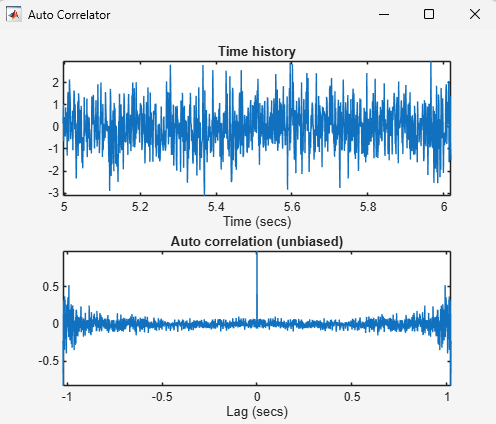
\includegraphics[width=\textwidth]{gaussian-noise-1-var.png}
        \caption{Variance = 1.}
        \label{fig:autocorr1}
    \end{subfigure}
    \hfill
    \begin{subfigure}[b]{0.48\textwidth}
        \centering
        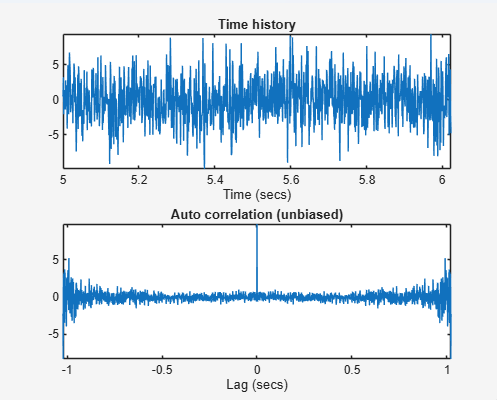
\includegraphics[width=\textwidth]{gaussian-noise-10-var.png}
        \caption{Variance = 10.}
        \label{fig:autocorr10}
    \end{subfigure}
    \caption{Autocorrelation of a zero-mean Gaussian source for two different variances. If we take the auto-correlation to be $R_{xx} (\tau) = \mathbb{E}(x(t)x(t+\tau))$,
    and we take the lag $\tau = 0$, we have $R_{xx}(0) = \mathbb{E}(x^2(t)) = \sigma^2$, the variance of the signal. The peak of the autocorrelation at zero lag is therefore equal to the variance, which is also the noise power for a zero-mean Gaussian source.}
    \label{fig:autocorr}
\end{figure}

\subsection*{Question 9}

A deterministic signal is completely specified by a mathematical expression, so its value at any time can be calculated exactly. For example, $x(t)=A\sin(2\pi ft+\phi)$ defines a sine wave once its amplitude, frequency, and phase are known.

A random signal is modeled as a stochastic process: its value at each time is a random variable, and each observed waveform is one realization of that process. Rather than predicting exact values, we characterize it statistically using probability distributions, mean, variance, autocorrelation, and power spectral density.

\section*{Part 2}

\subsection*{Question 1}
\begin{figure}[H]
    \centering
    \begin{subfigure}[b]{0.48\textwidth}
        \centering
        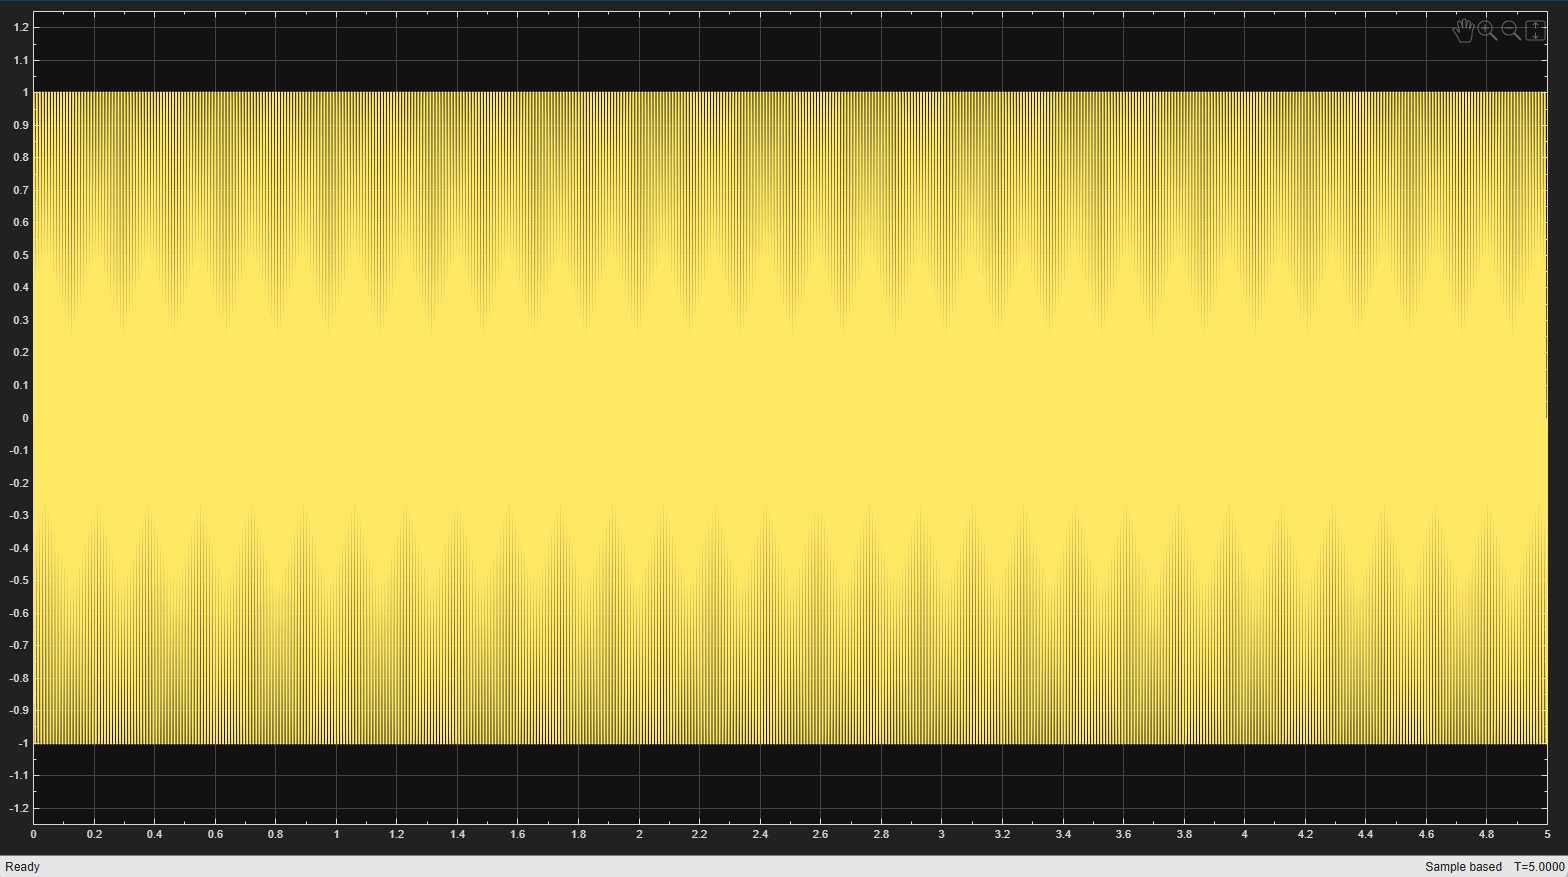
\includegraphics[width=\textwidth]{q2_1_source_scope.png}
        \caption{Time domain.}
        \label{fig:q2-1-source-scope}
    \end{subfigure}
    \hfill
    \begin{subfigure}[b]{0.48\textwidth}
        \centering
        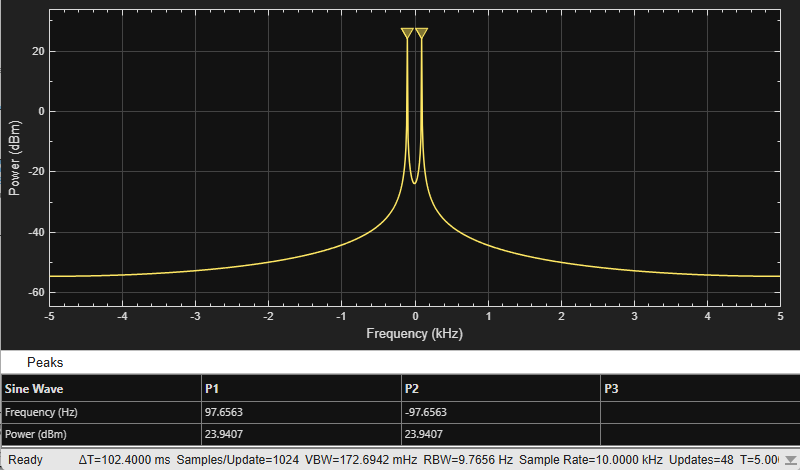
\includegraphics[width=\textwidth]{q2_1_source_spectrum.png}
        \caption{Spectrum.}
        \label{fig:q2-1-source-spectrum}
    \end{subfigure}
    \caption{Sine wave source (100 samples per period, $T_s = 10^{-4}$\,s, i.e. 100\,Hz). The bandwidth should be 0Hz for a pure sine wave, but it appears to be non-zero here due to finite FFT resolution.
    The total power is about $23.94\text{dBm} \times 2 = 26.94\text{dBm}$.}
    \label{fig:q2-1-source}
\end{figure}

\subsection*{Question 2}

\begin{figure}[H]
    \centering
    \begin{subfigure}[b]{0.48\textwidth}
        \centering
        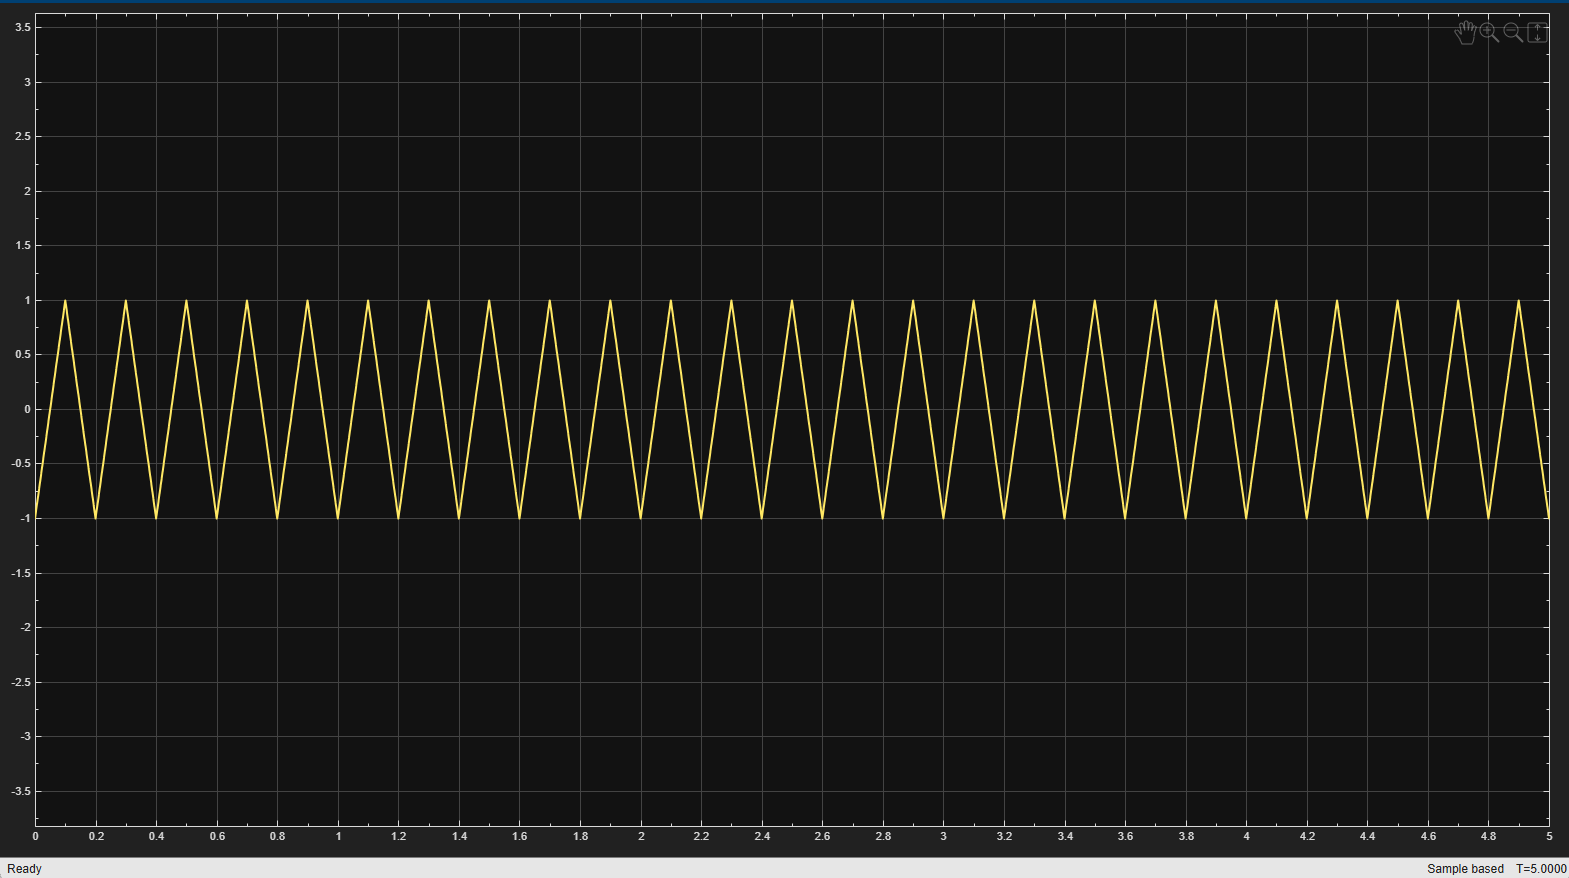
\includegraphics[width=\textwidth]{q2_2_source_scope_gain_10_fc_100.png}
        \caption{Time domain.}
        \label{fig:q2-2-source-scope}
    \end{subfigure}
    \hfill
    \begin{subfigure}[b]{0.48\textwidth}
        \centering
        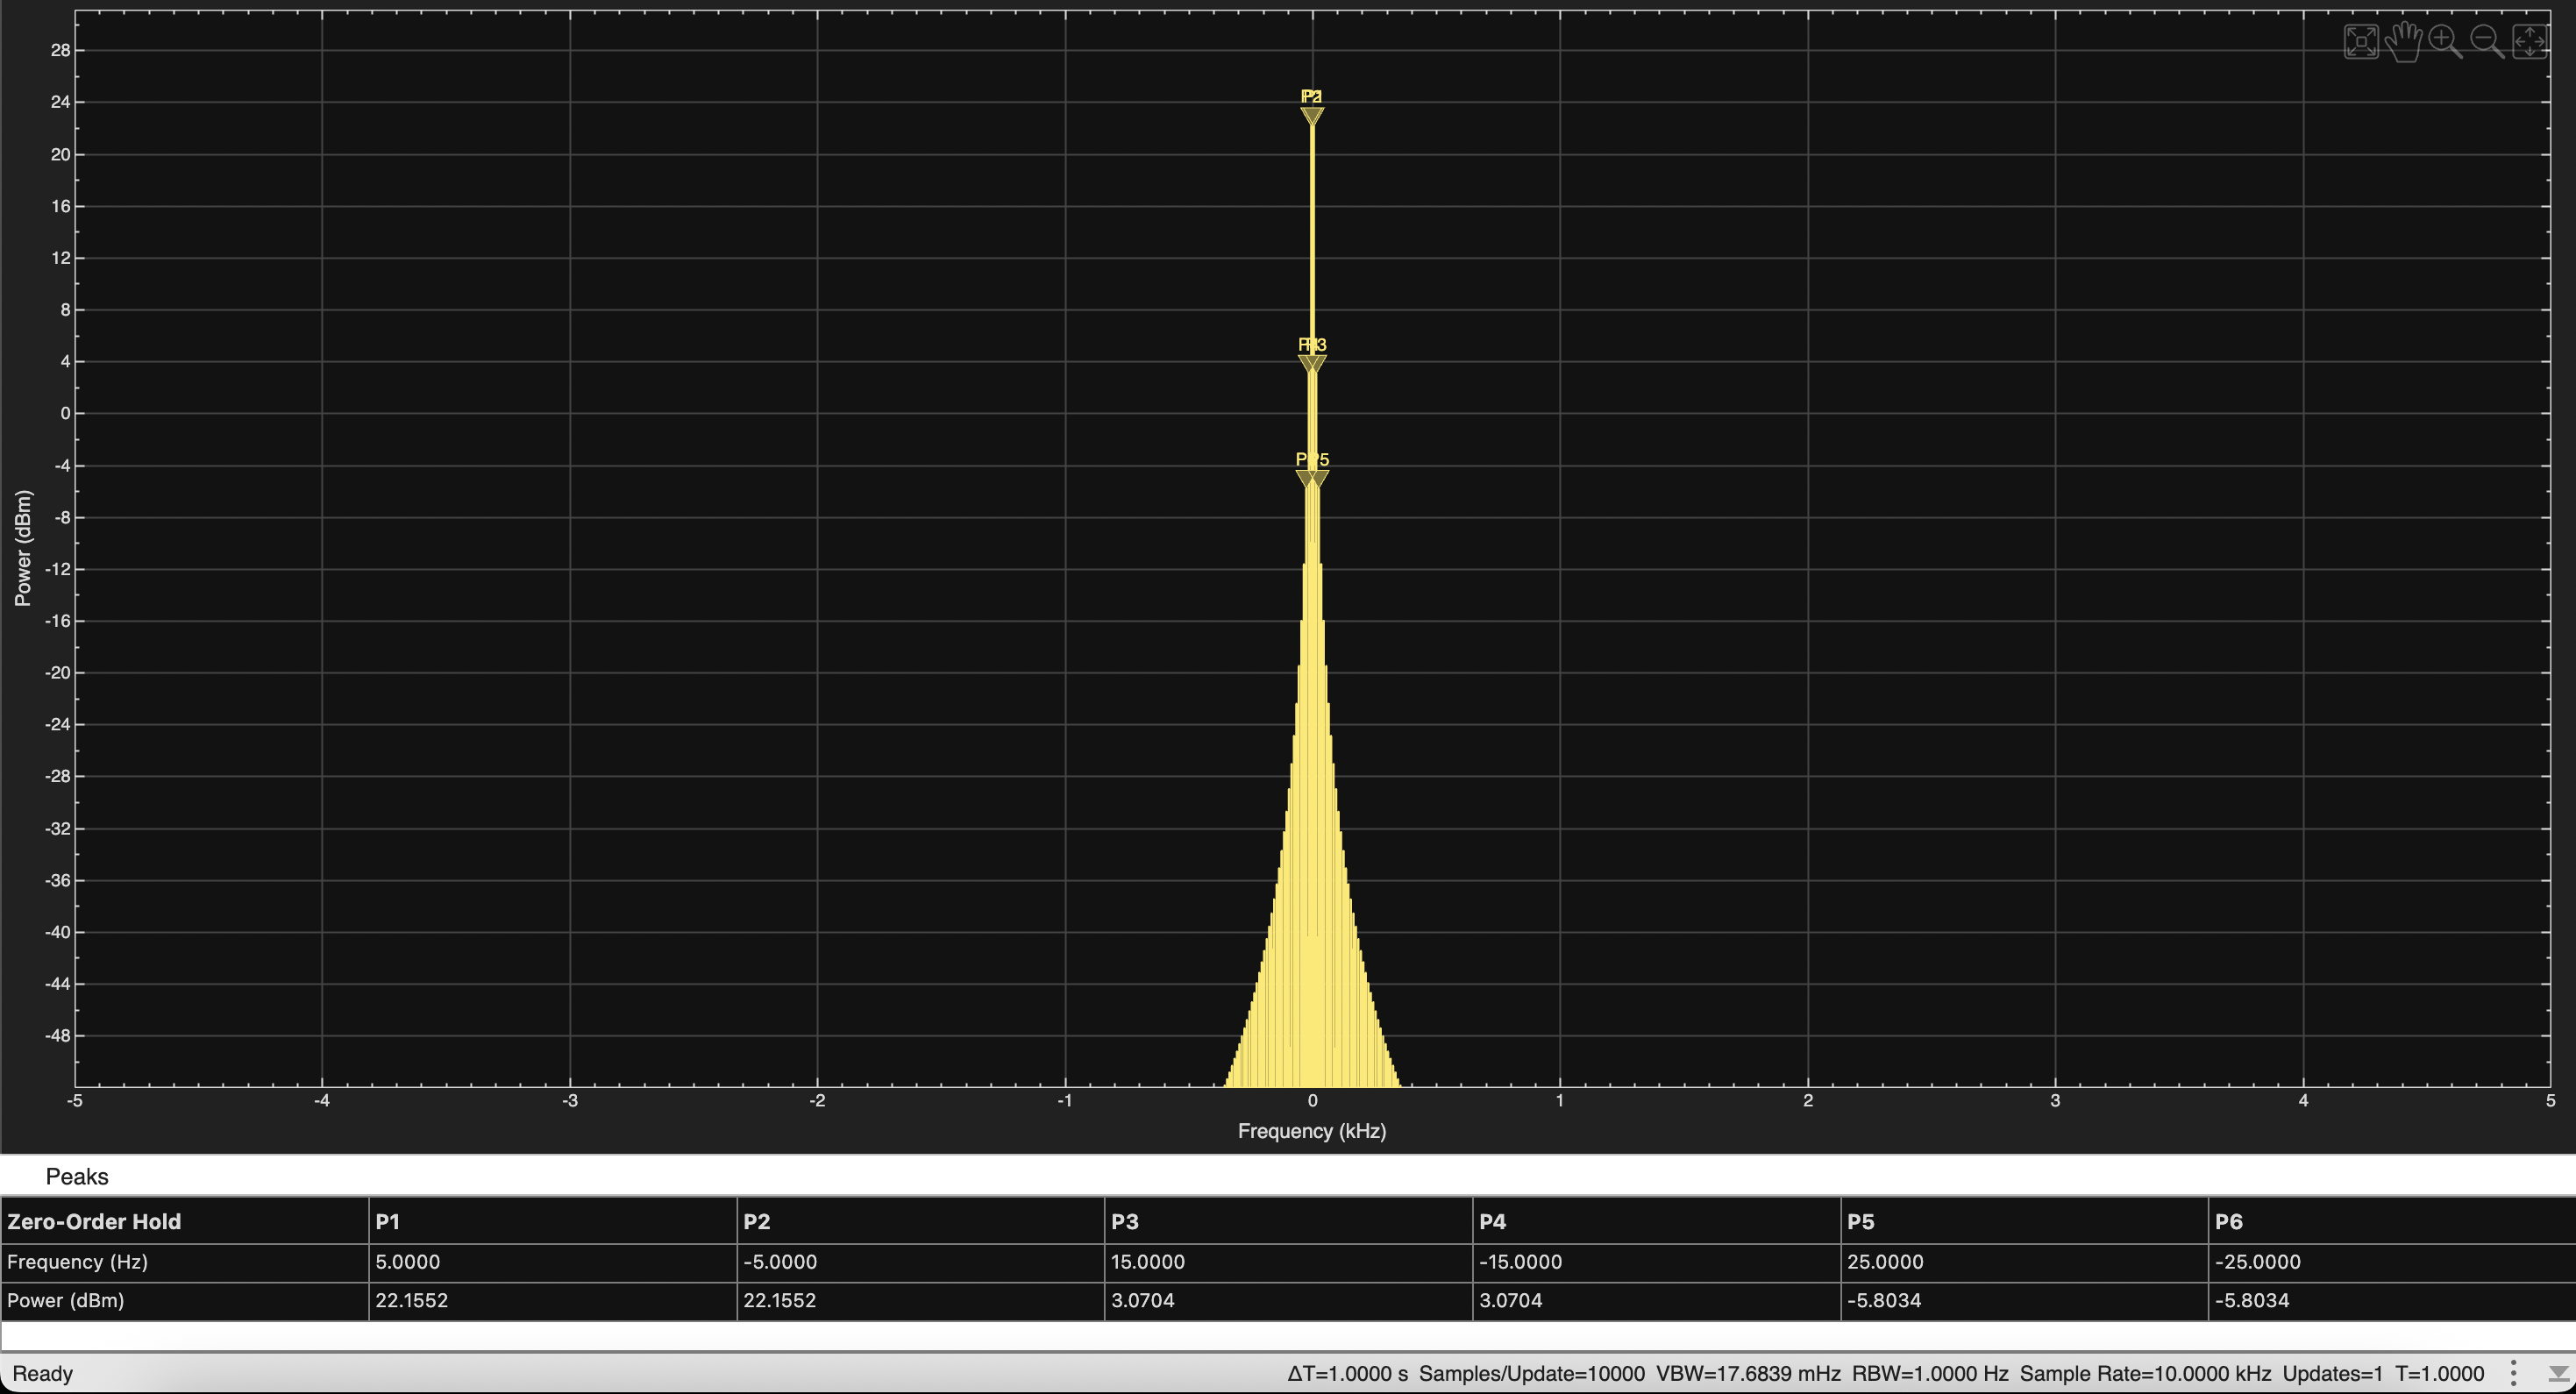
\includegraphics[width=\textwidth]{q2_2_source_spectrum_gain_10_fc_100.png}
        \caption{Spectrum.}
        \label{fig:q2-2-source-spectrum}
    \end{subfigure}
    \caption{Triangular wave source at 5\,Hz ($T_s = 10^{-4}$\,s). The bandwidth of a triangle wave is theoretically infinite, but we do not observe this due to finite FFT resolution.
    The estimated total power is the sum of the power of the 3 first harmonics: $P_{total} = 22.1552 + 3.0704 - 5.8034 = 22.21\text{dBm}$.}
    \label{fig:q2-2-source}
\end{figure}

\subsection*{Question 3}
\begin{figure}[H]
    \centering
    \begin{subfigure}[b]{0.48\textwidth}
        \centering
        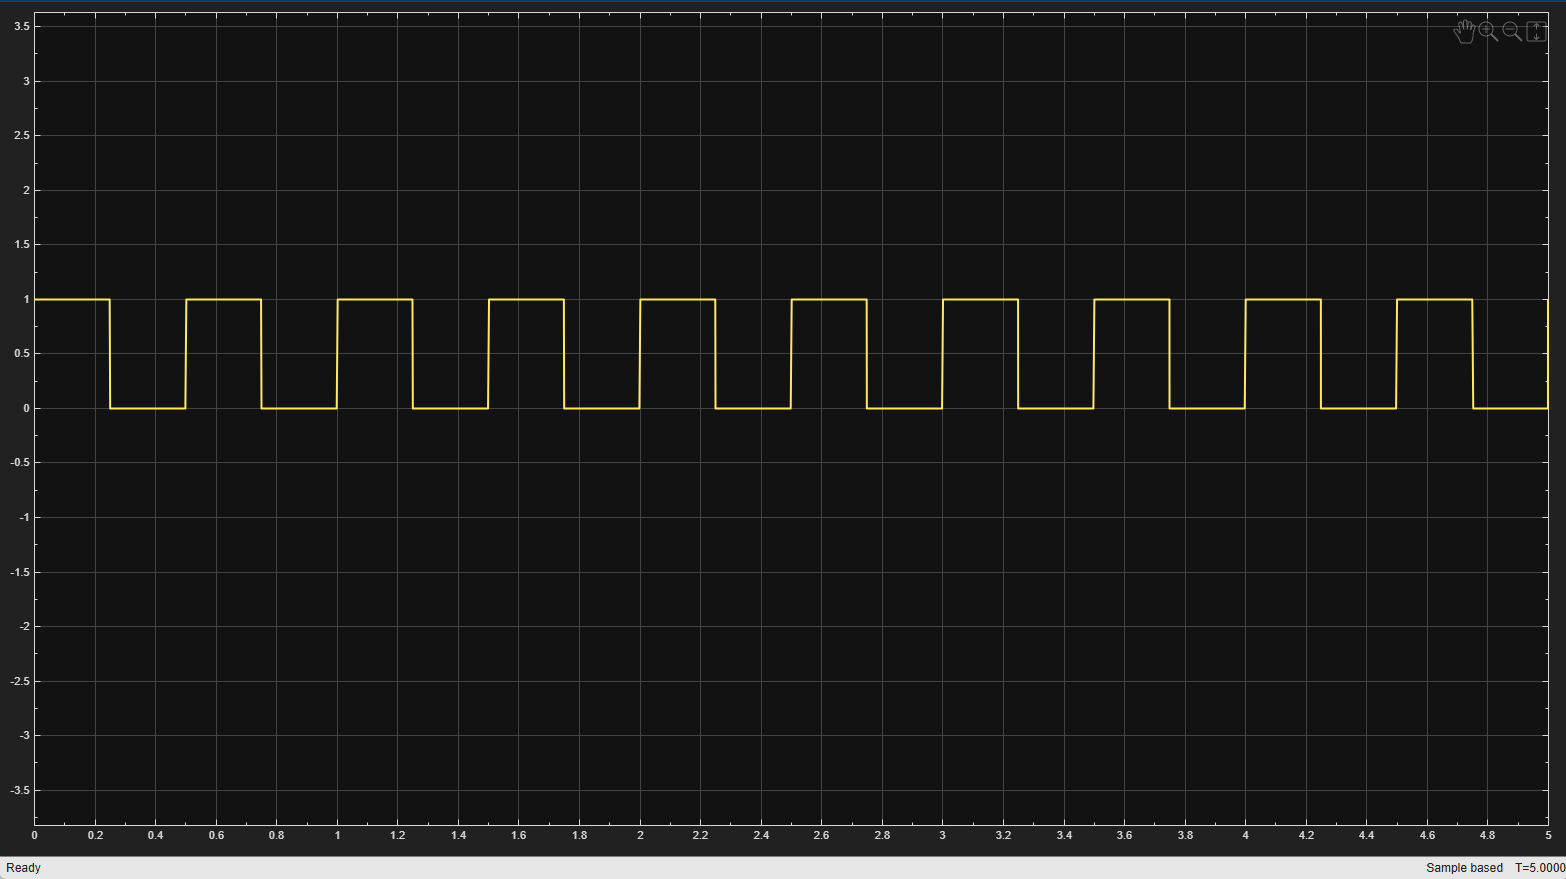
\includegraphics[width=\textwidth]{q2_3_source_scope_gain_10_fc_100.png}
        \caption{Time domain.}
        \label{fig:q2-3-source-scope}
    \end{subfigure}
    \hfill
    \begin{subfigure}[b]{0.48\textwidth}
        \centering
        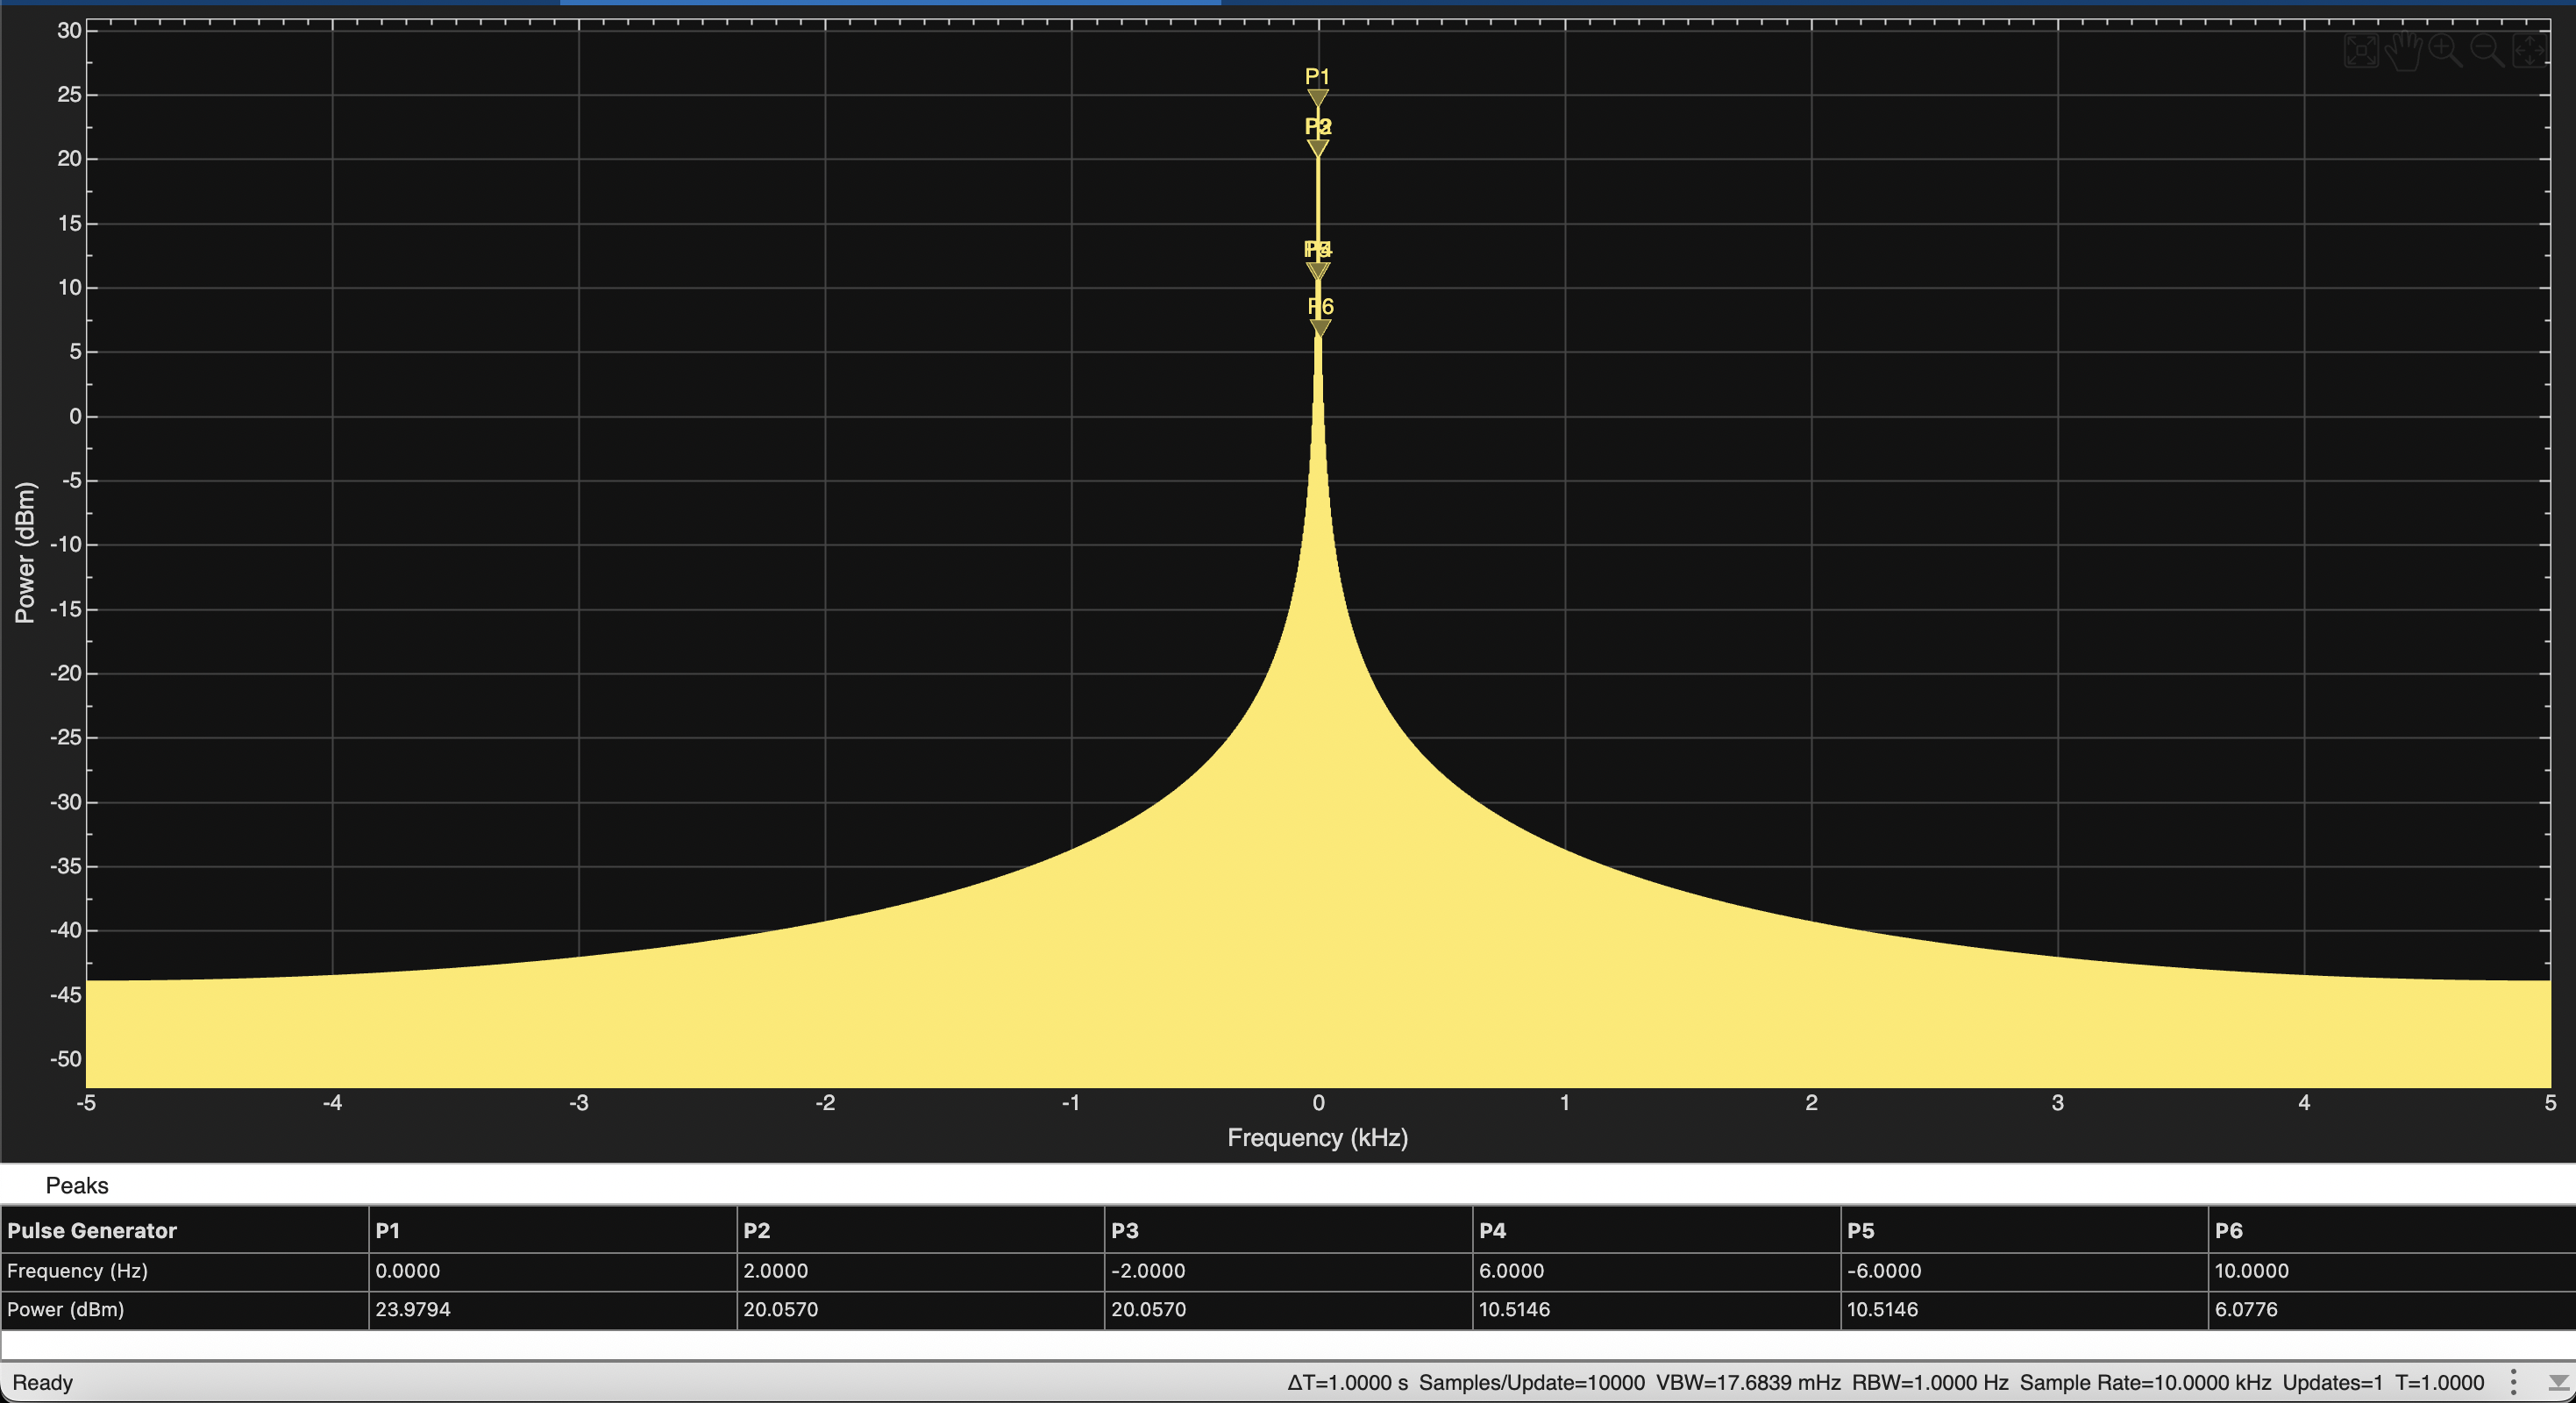
\includegraphics[width=\textwidth]{q2_3_source_spectrum_gain_10_fc_100.png}
        \caption{Spectrum.}
        \label{fig:q2-3-source-spectrum}
    \end{subfigure}
    \caption{50\% duty cycle square wave source (period 5000 samples, $T_s = 10^{-4}$\,s, i.e. 2\,Hz). The bandwidth of a square wave is theoretically infinite, but we do not observe this due to finite FFT resolution.
    In our spectrum, we observe a bandwidth of 10kHz. The total power is estimated to be $P_{total} = 23.9794 + 20.0570 \times 2 + 10.5146 \times 2 = 26.77\text{dBm}$.}
    \label{fig:q2-3-source}
\end{figure}

\subsection*{Question 4}
\begin{figure}[H]
    \centering
    \begin{subfigure}[b]{0.48\textwidth}
        \centering
        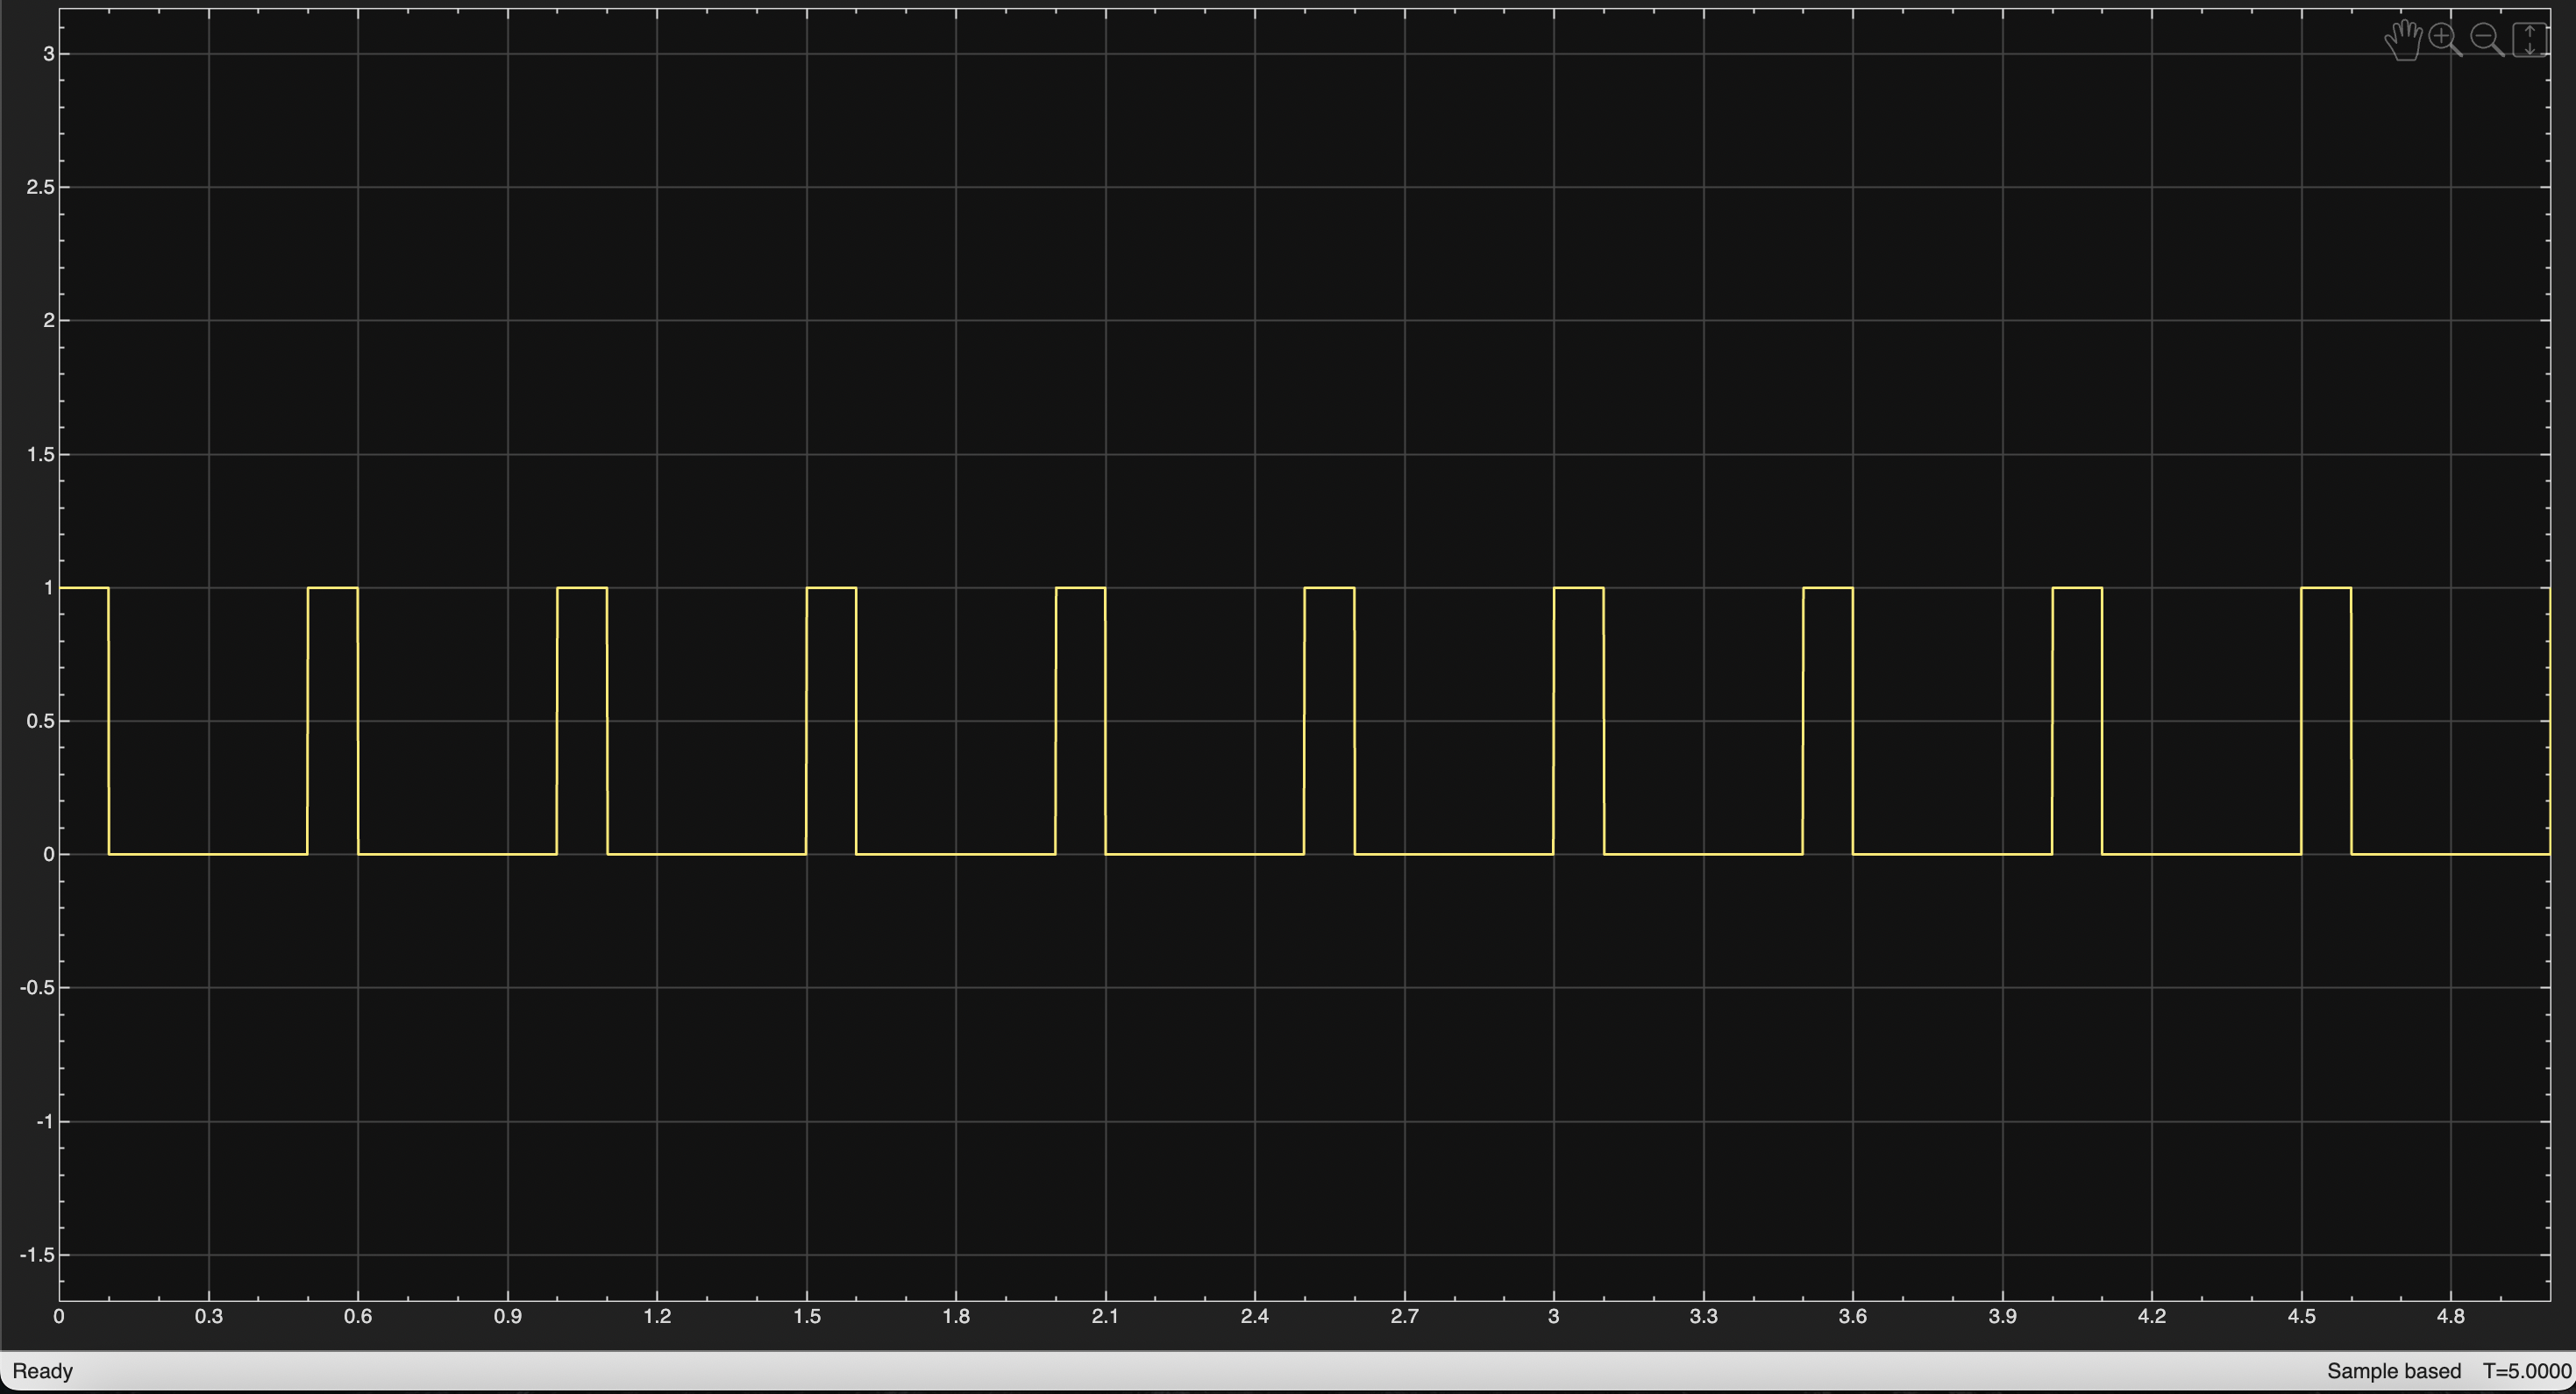
\includegraphics[width=\textwidth]{q2_4_source_scope_gain_10_fc_100.png}
        \caption{Time domain.}
        \label{fig:q2-4-source-scope}
    \end{subfigure}
    \hfill
    \begin{subfigure}[b]{0.48\textwidth}
        \centering
        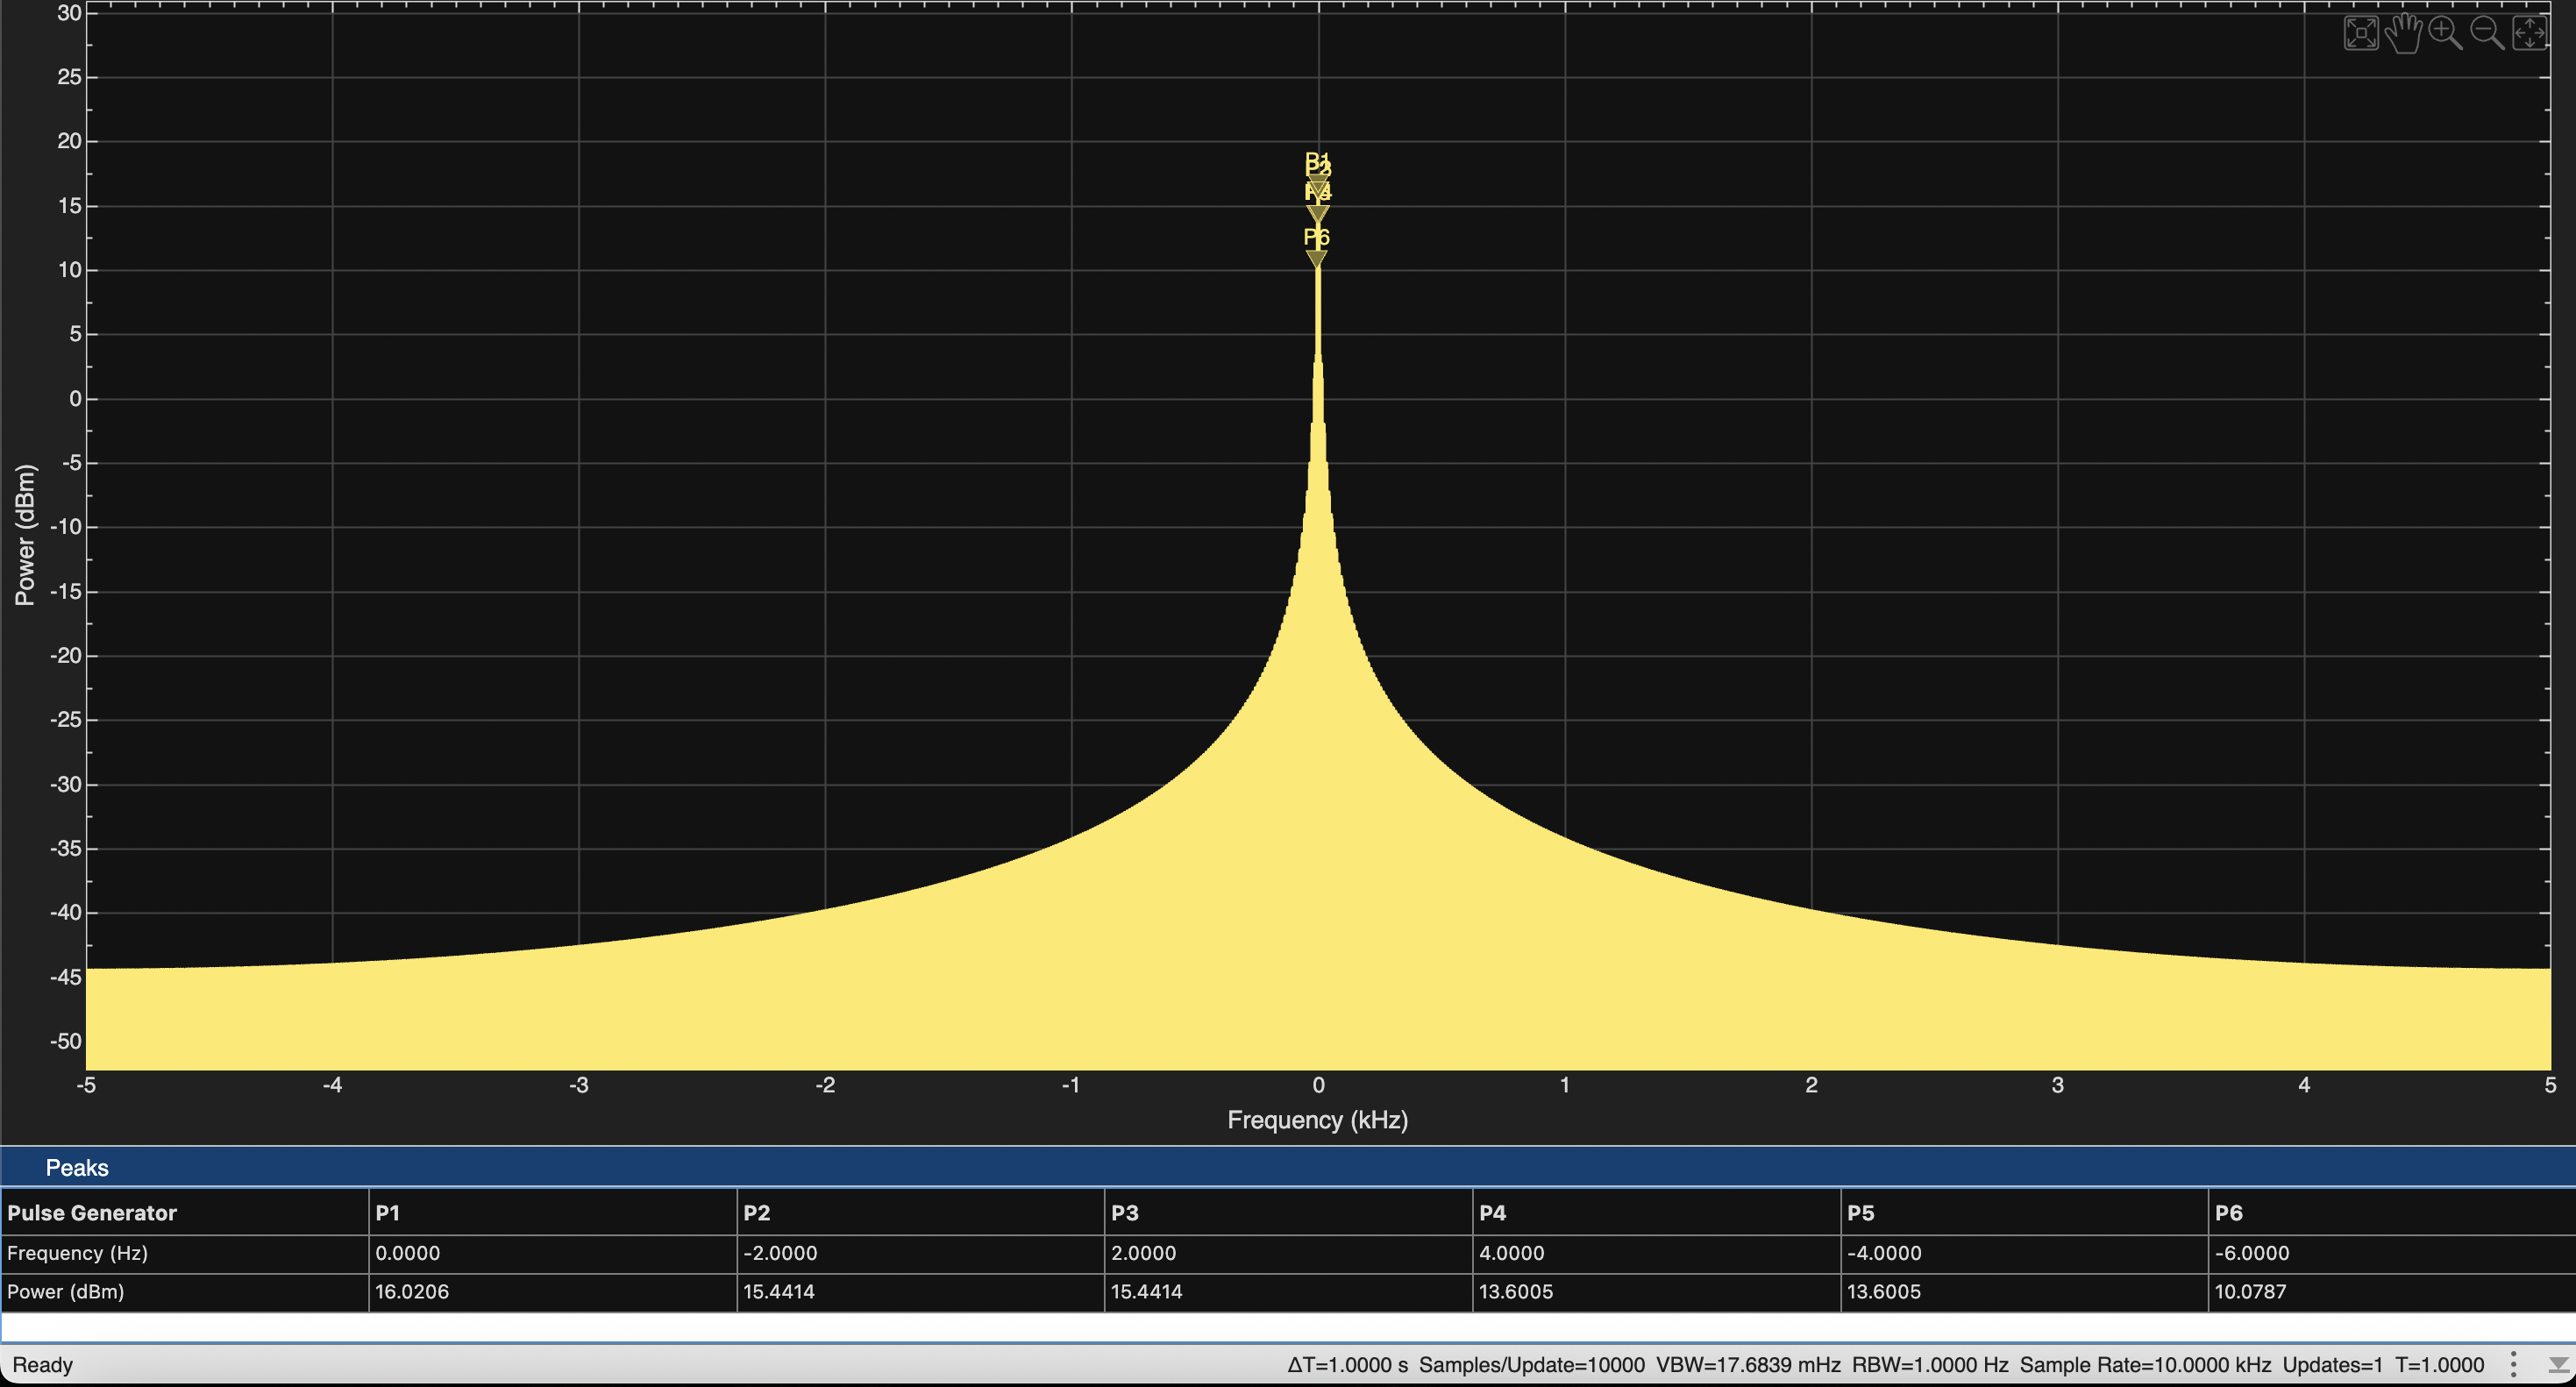
\includegraphics[width=\textwidth]{q2_4_source_spectrum_gain_10_fc_100.png}
        \caption{Spectrum.}
        \label{fig:q2-4-source-spectrum}
    \end{subfigure}
    \caption{20\% duty cycle square wave source at Slider Gain 10 and $F_c = 100$\,Hz. The bandwidth of a square wave is theoretically infinite, but we do not observe this due to finite FFT resolution.
    In our spectrum, we observe a bandwidth of 10kHz. The total power is estimated to be $P_{total} = 16.0206 + 15.4414 \times 2 + 13.6005 \times 2 = 21.93\text{dBm}$.}
    \label{fig:q2-4-source}
\end{figure}

\subsection*{Question 5}
\begin{figure}[H]
    \centering
    \begin{subfigure}[b]{0.48\textwidth}
        \centering
        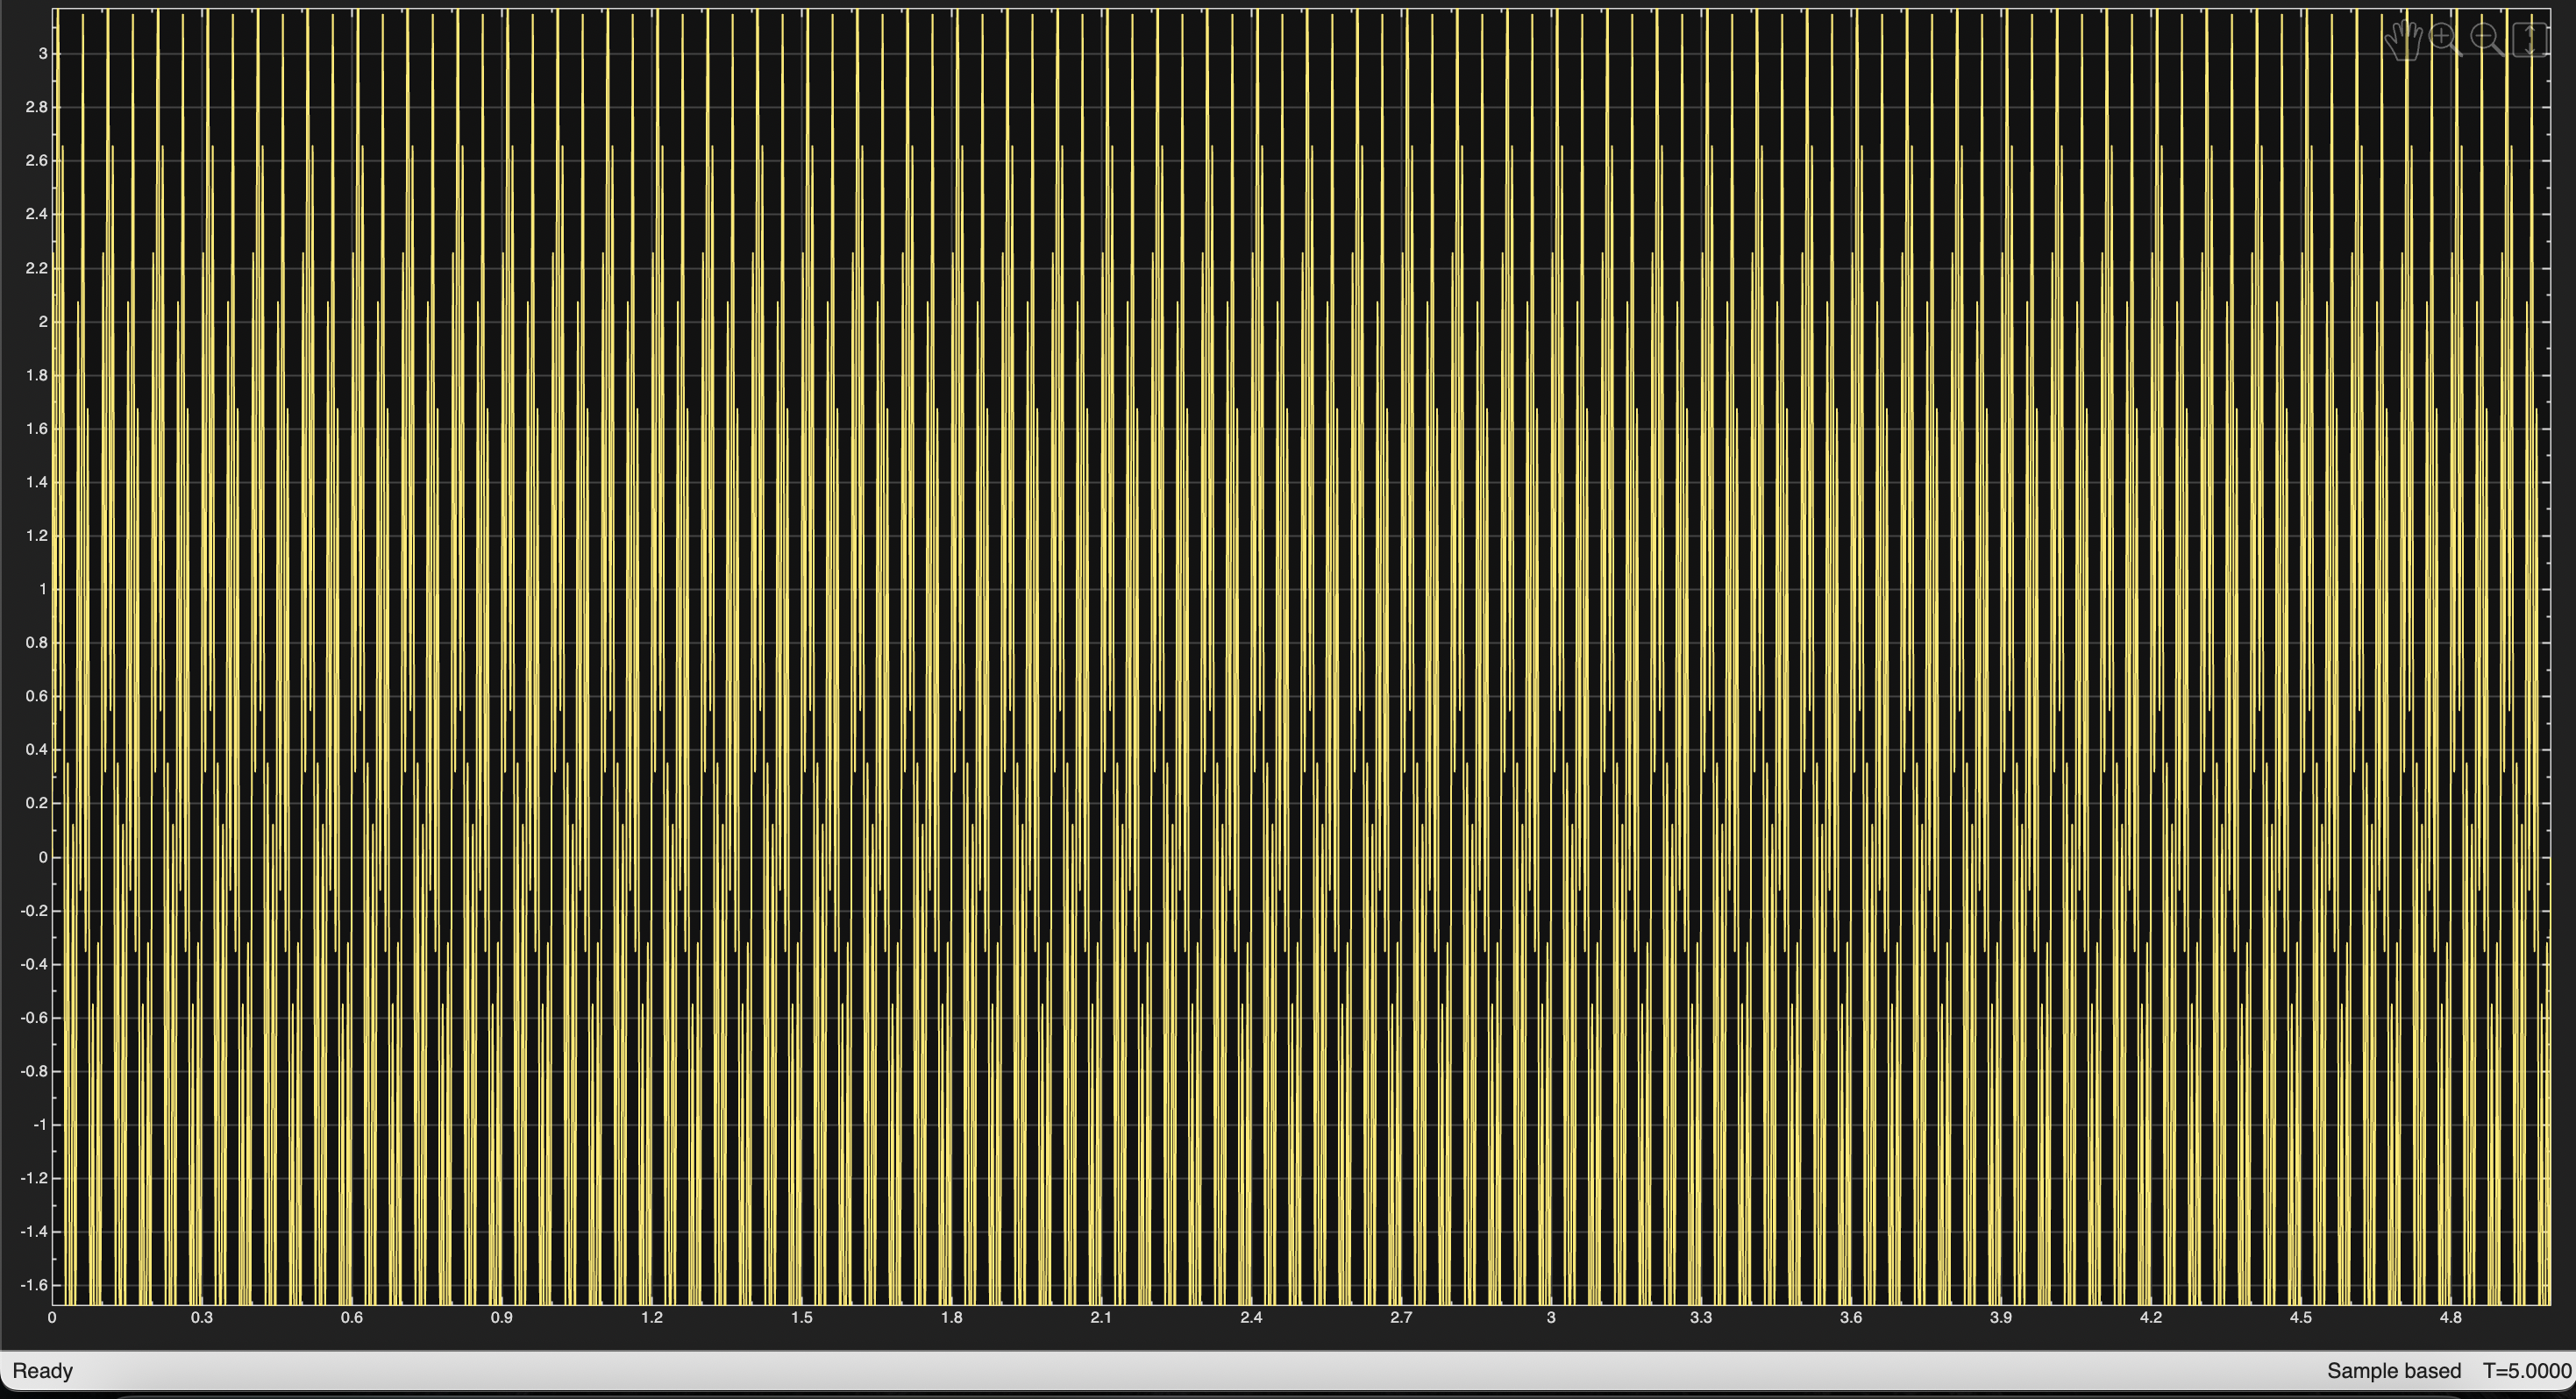
\includegraphics[width=\textwidth]{q2_5_source_scope_gain_10_fc_100.png}
        \caption{Time domain.}
        \label{fig:q2-5-source-scope}
    \end{subfigure}
    \hfill
    \begin{subfigure}[b]{0.48\textwidth}
        \centering
        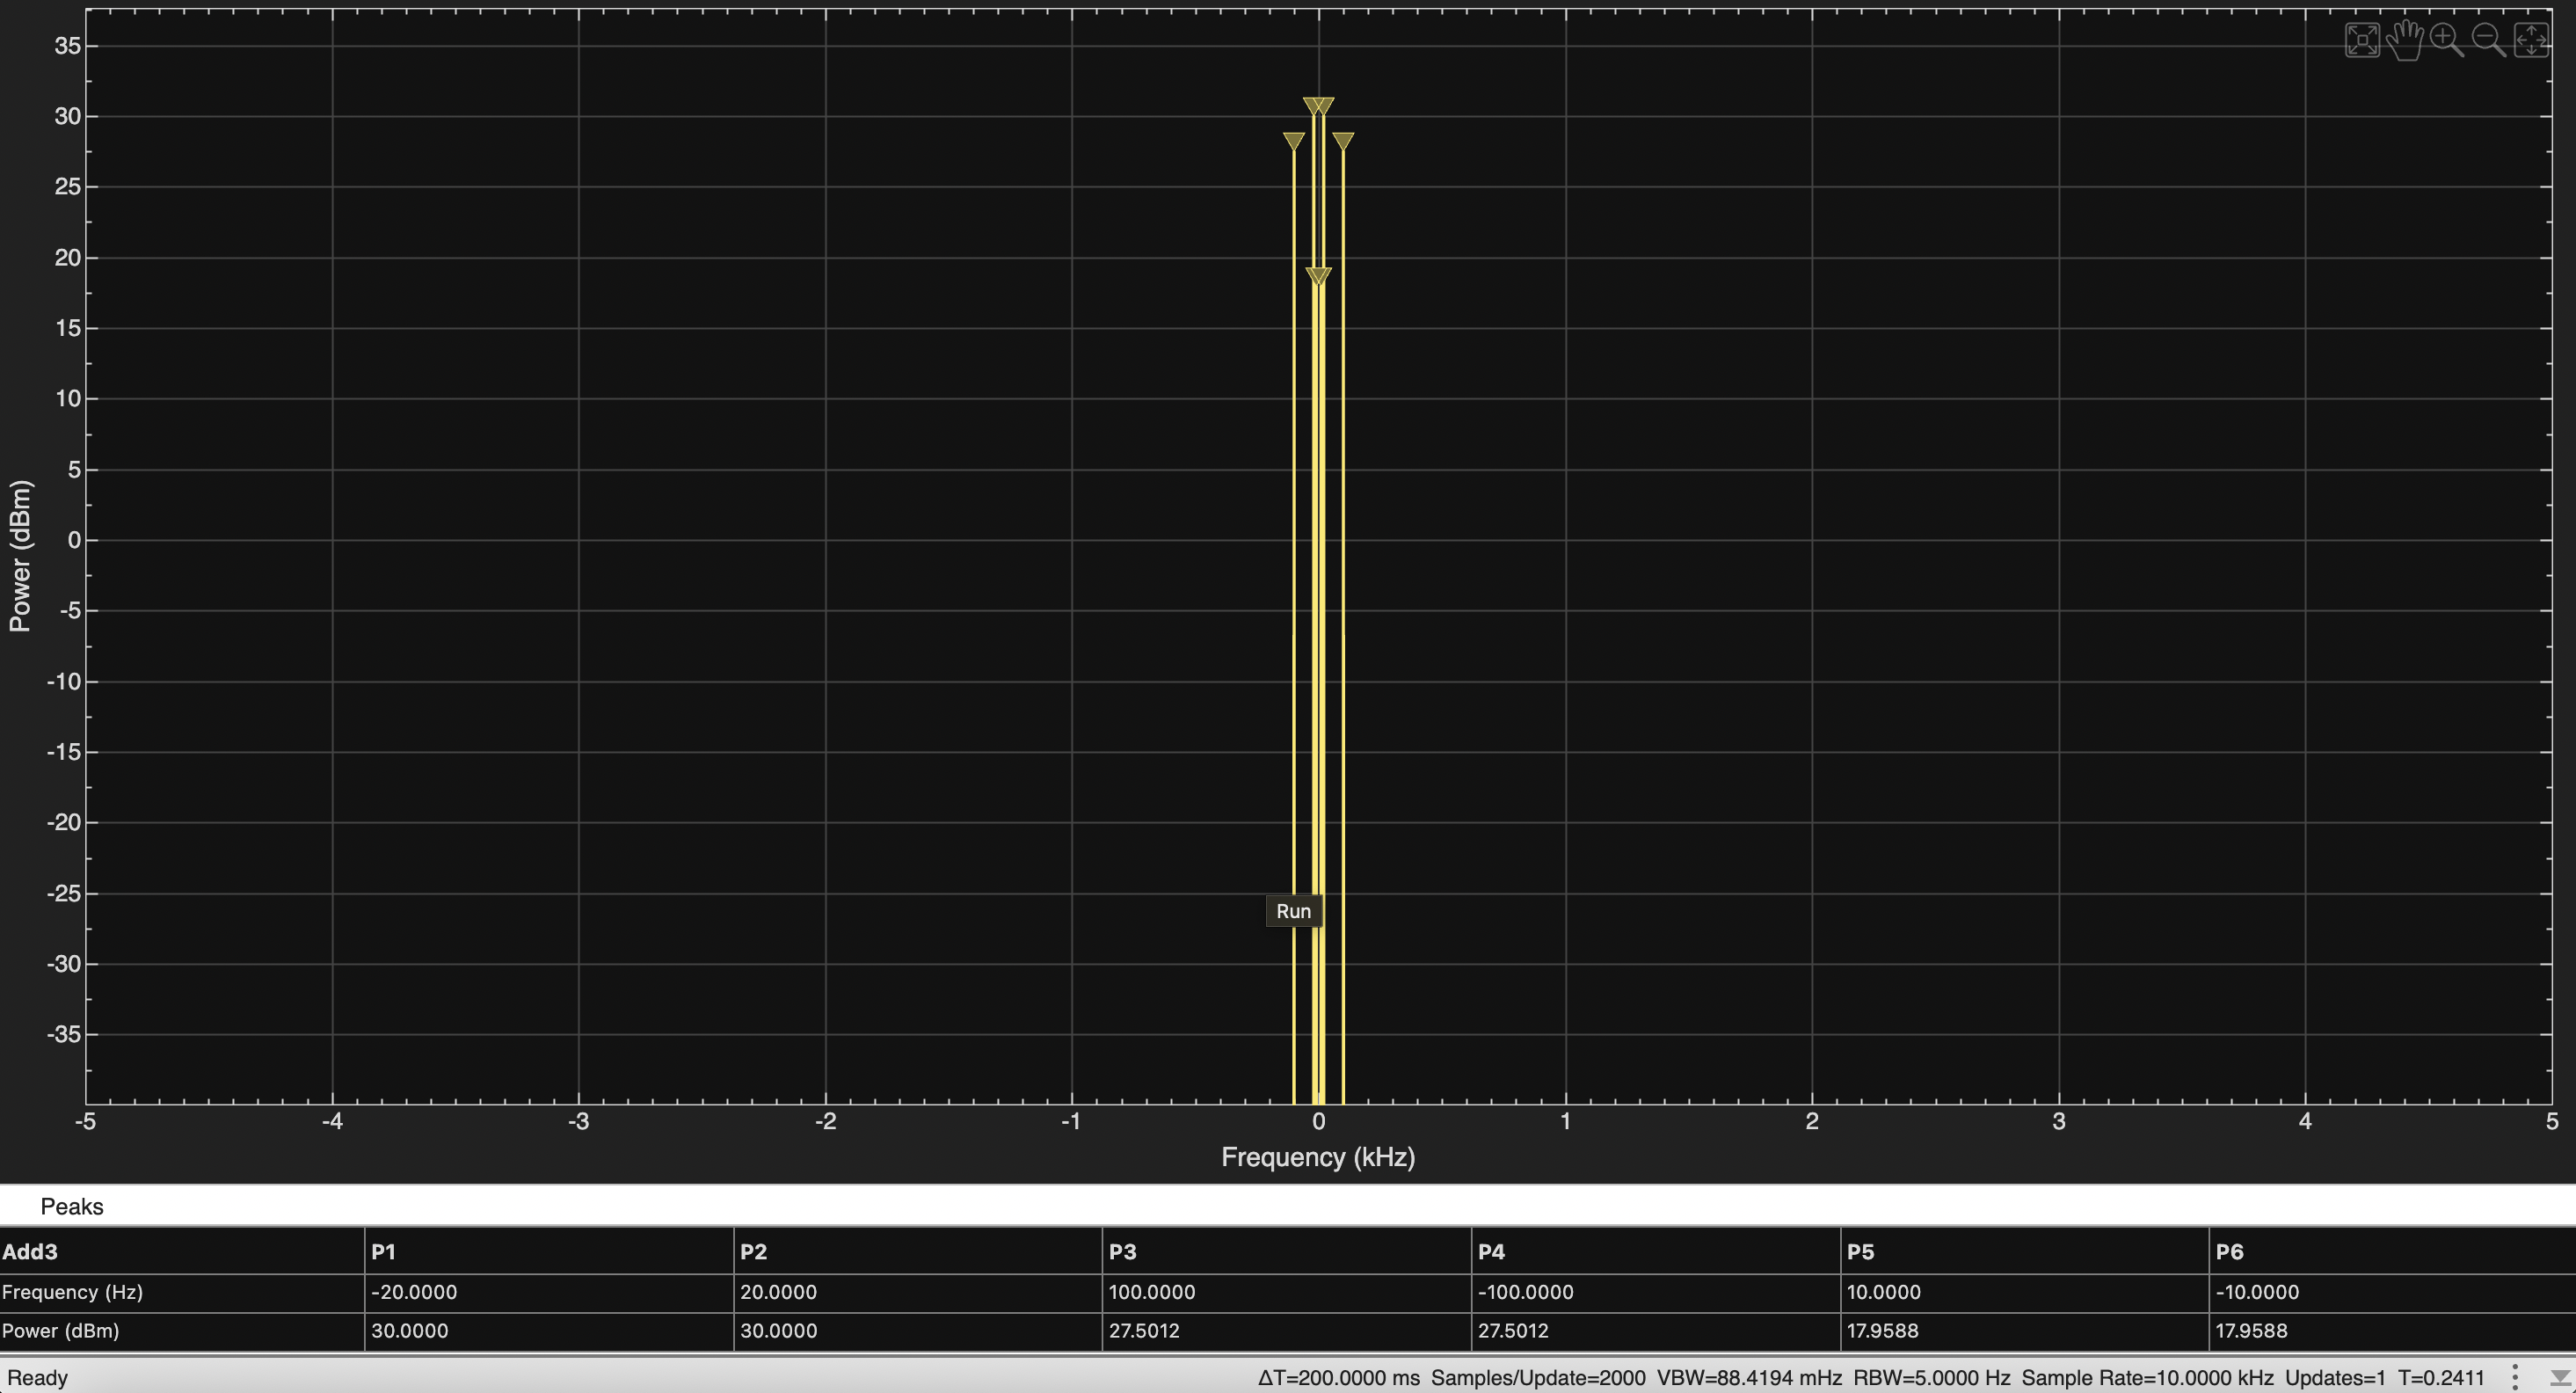
\includegraphics[width=\textwidth]{q2_5_source_spectrum_gain_10_fc_100.png}
        \caption{Spectrum.}
        \label{fig:q2-5-source-spectrum}
    \end{subfigure}
    \label{fig:q2-5-source}
    \caption{Sum-of-sines source at Slider Gain 10 and $F_c = 100$\,Hz. The theoretical bandwidth is twice the maximum frequency of the sine waves. In this case, it's }
\end{figure}

\subsection*{Question 6}

Adding noise to the original signal has changed both the time domain and the frequency domain signal by: making the curves noisy in time and by introducing random power in non-fundamental frequencies as well as some extra power in the fundamental frequencies.

\begin{figure}[H]
    \centering
    \begin{subfigure}[b]{0.48\textwidth}
        \centering
        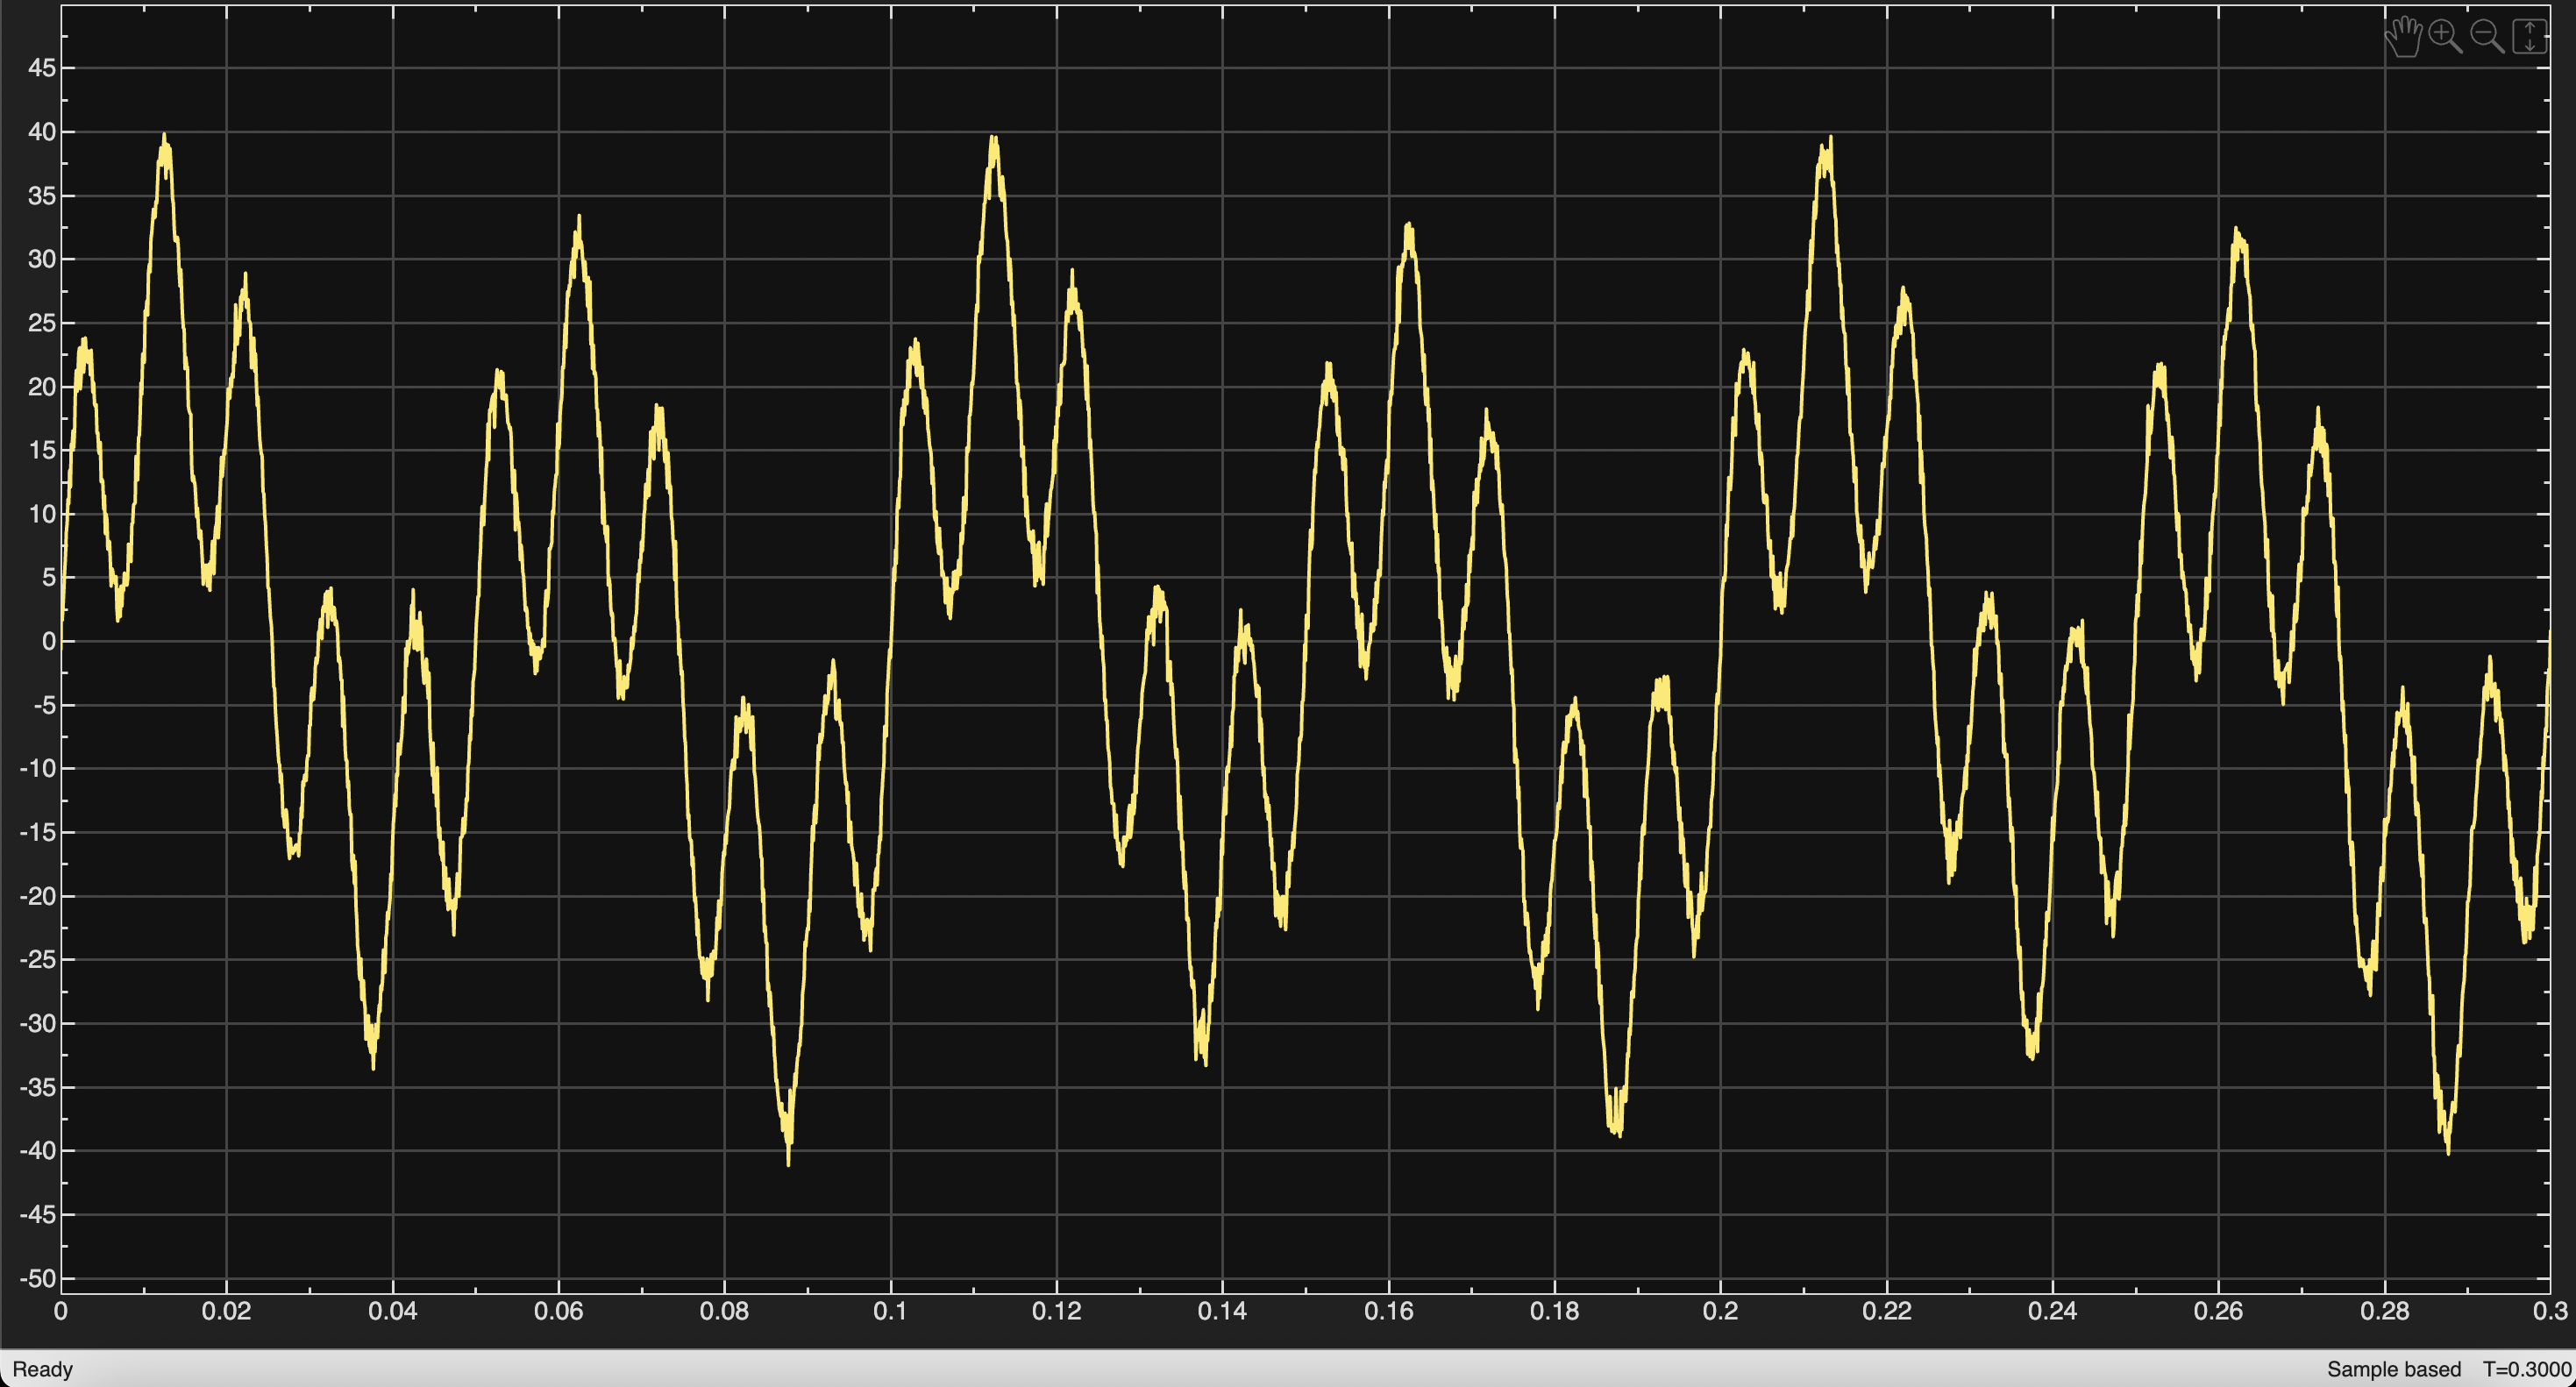
\includegraphics[width=\textwidth]{q2_5_rx_scope_gain_10_fc_100.png}
        \caption{Sum of three sine waves, time domain.}
        \label{fig:q2-5-rx-scope}
    \end{subfigure}
    \hfill
    \begin{subfigure}[b]{0.48\textwidth}
        \centering
        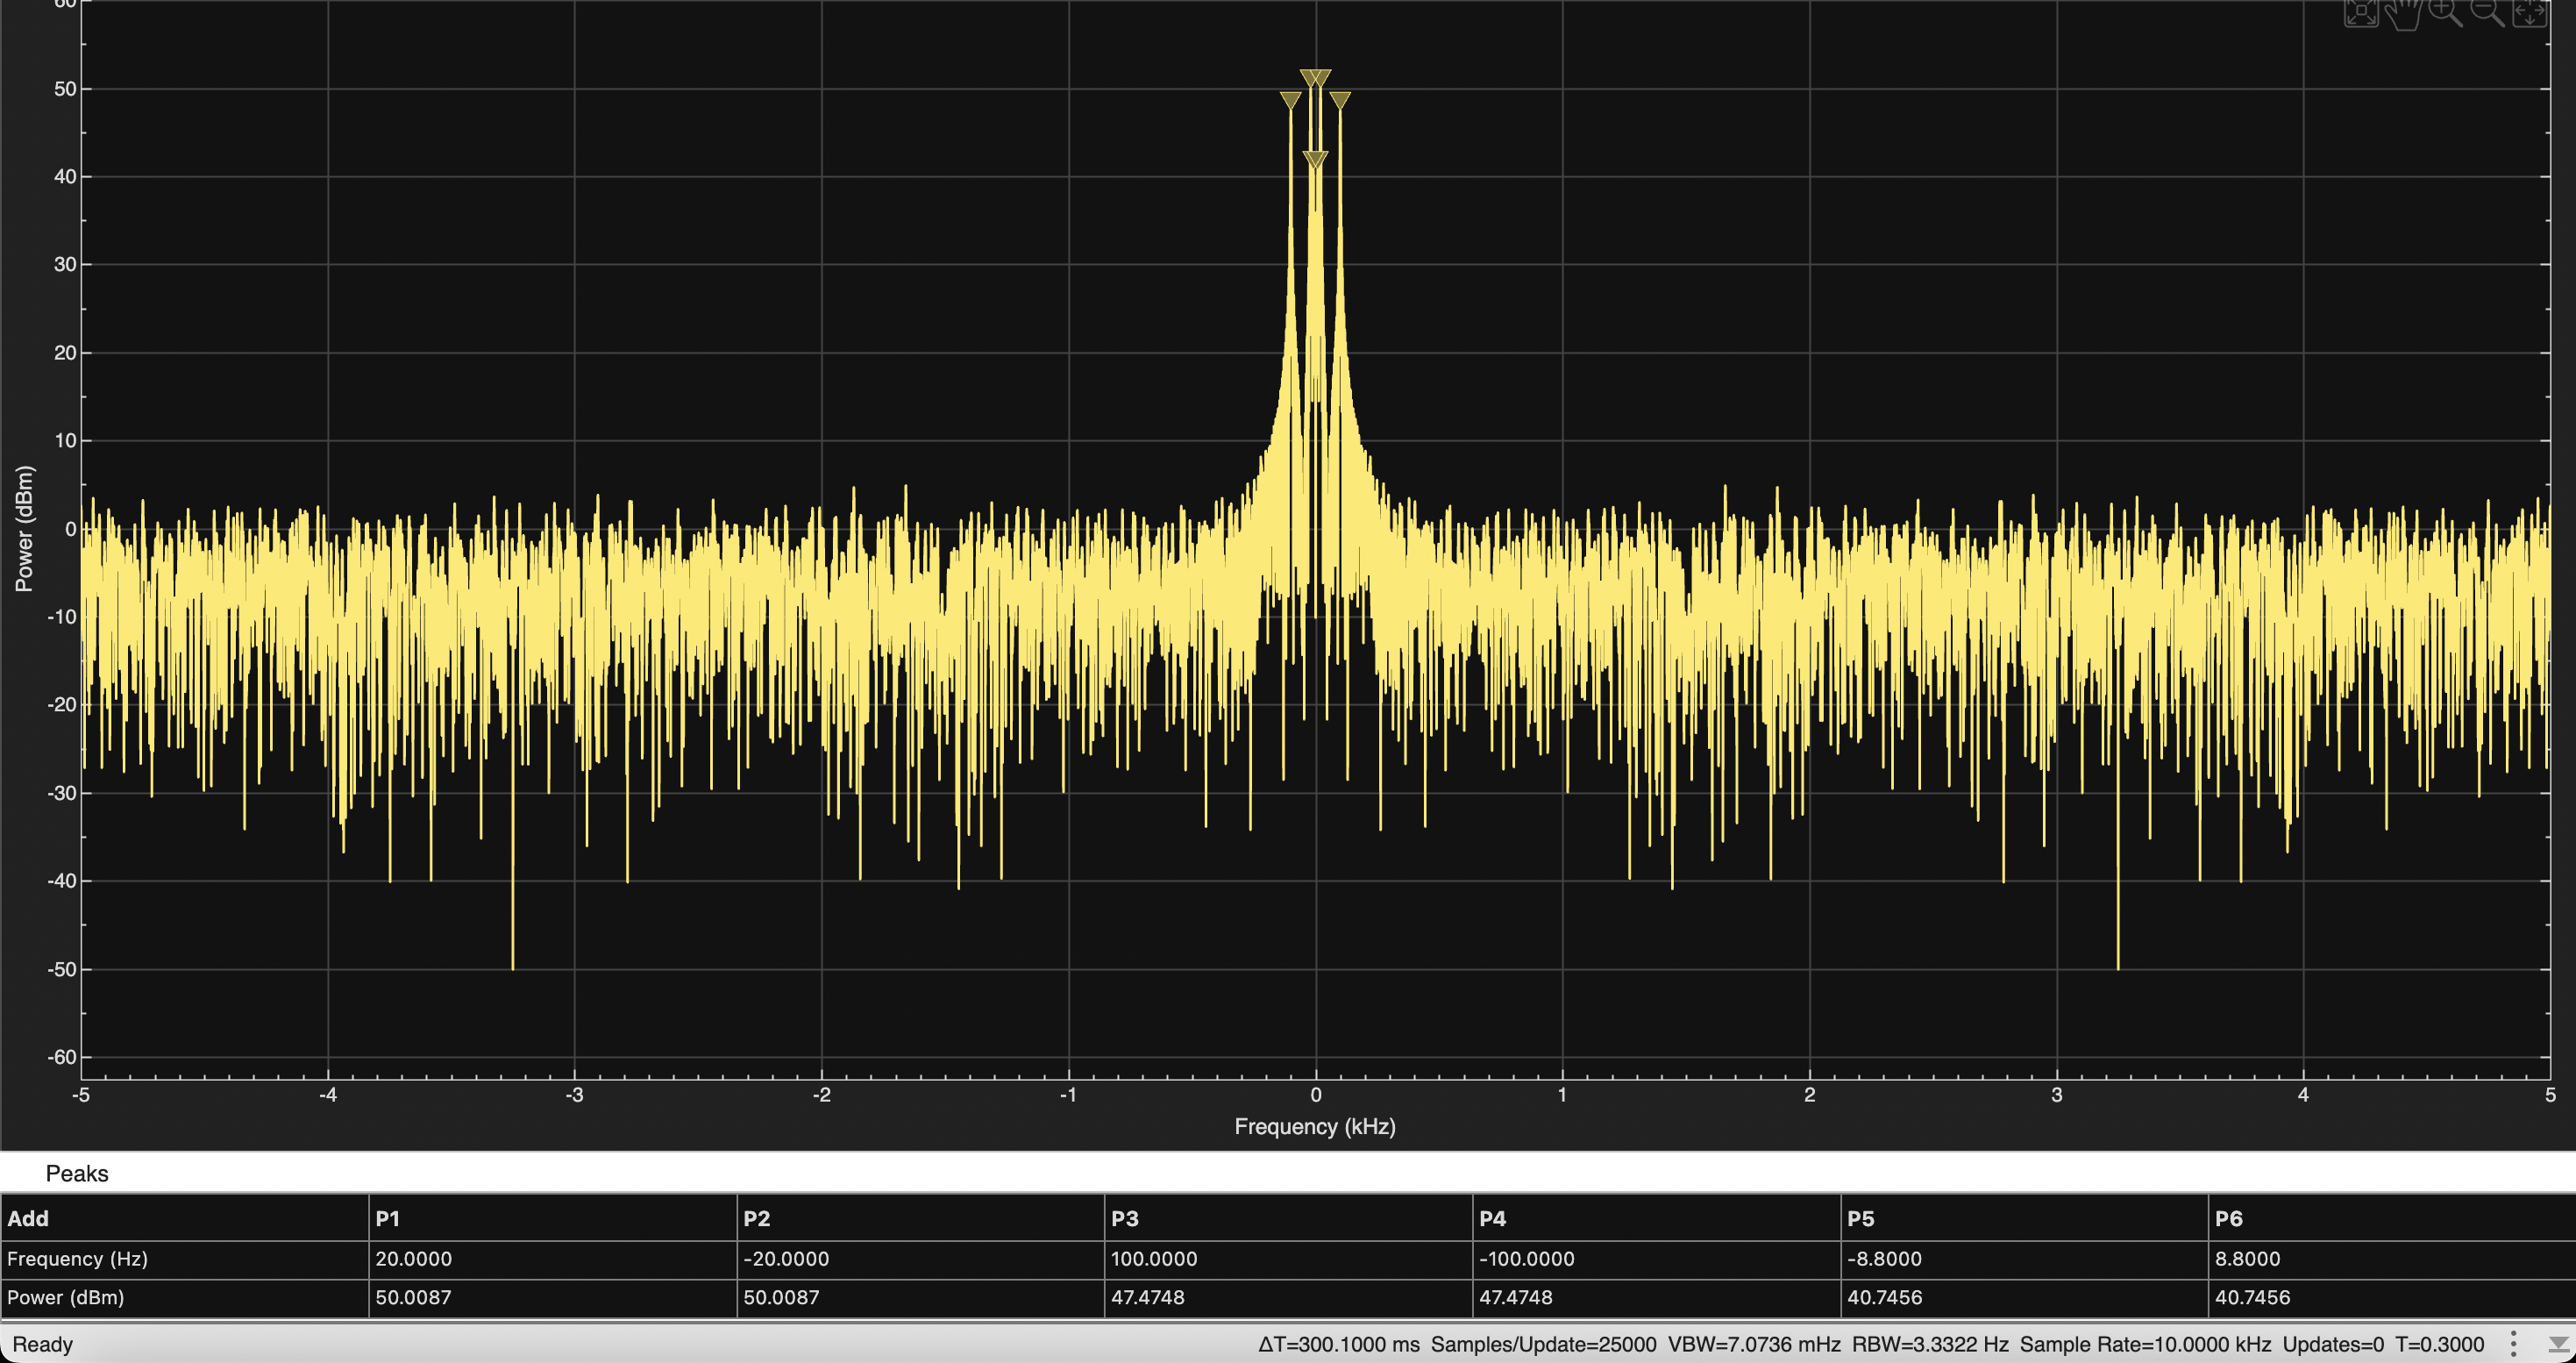
\includegraphics[width=\textwidth]{q2_5_rx_spectrum_gain_10_fc_100.png}
        \caption{Sum of three sine waves, spectrum.}
        \label{fig:q2-5-rx-spectrum}
    \end{subfigure}
    \caption{Received sum of three sine waves with added Gaussian noise at Slider Gain 10 and $F_c=100$\,Hz.}
    \label{fig:q2-5-rx}
\end{figure}

\subsection*{Question 7}
Since the filter is a low-pass filter with a cutoff frequency of 100Hz, the resulting frequency domain signal is a smoother curve with clearly pronounced peaks
at the expected frequencies (those observed in question 5). This is because the filter removes the high-frequency noise (although, not all of it).
The resulting time-domain signal is also a little smoother (there is still some roughness due to low-frequency noise still being present).

\begin{figure}[H]
    \centering
    \begin{subfigure}[b]{0.48\textwidth}
        \centering
        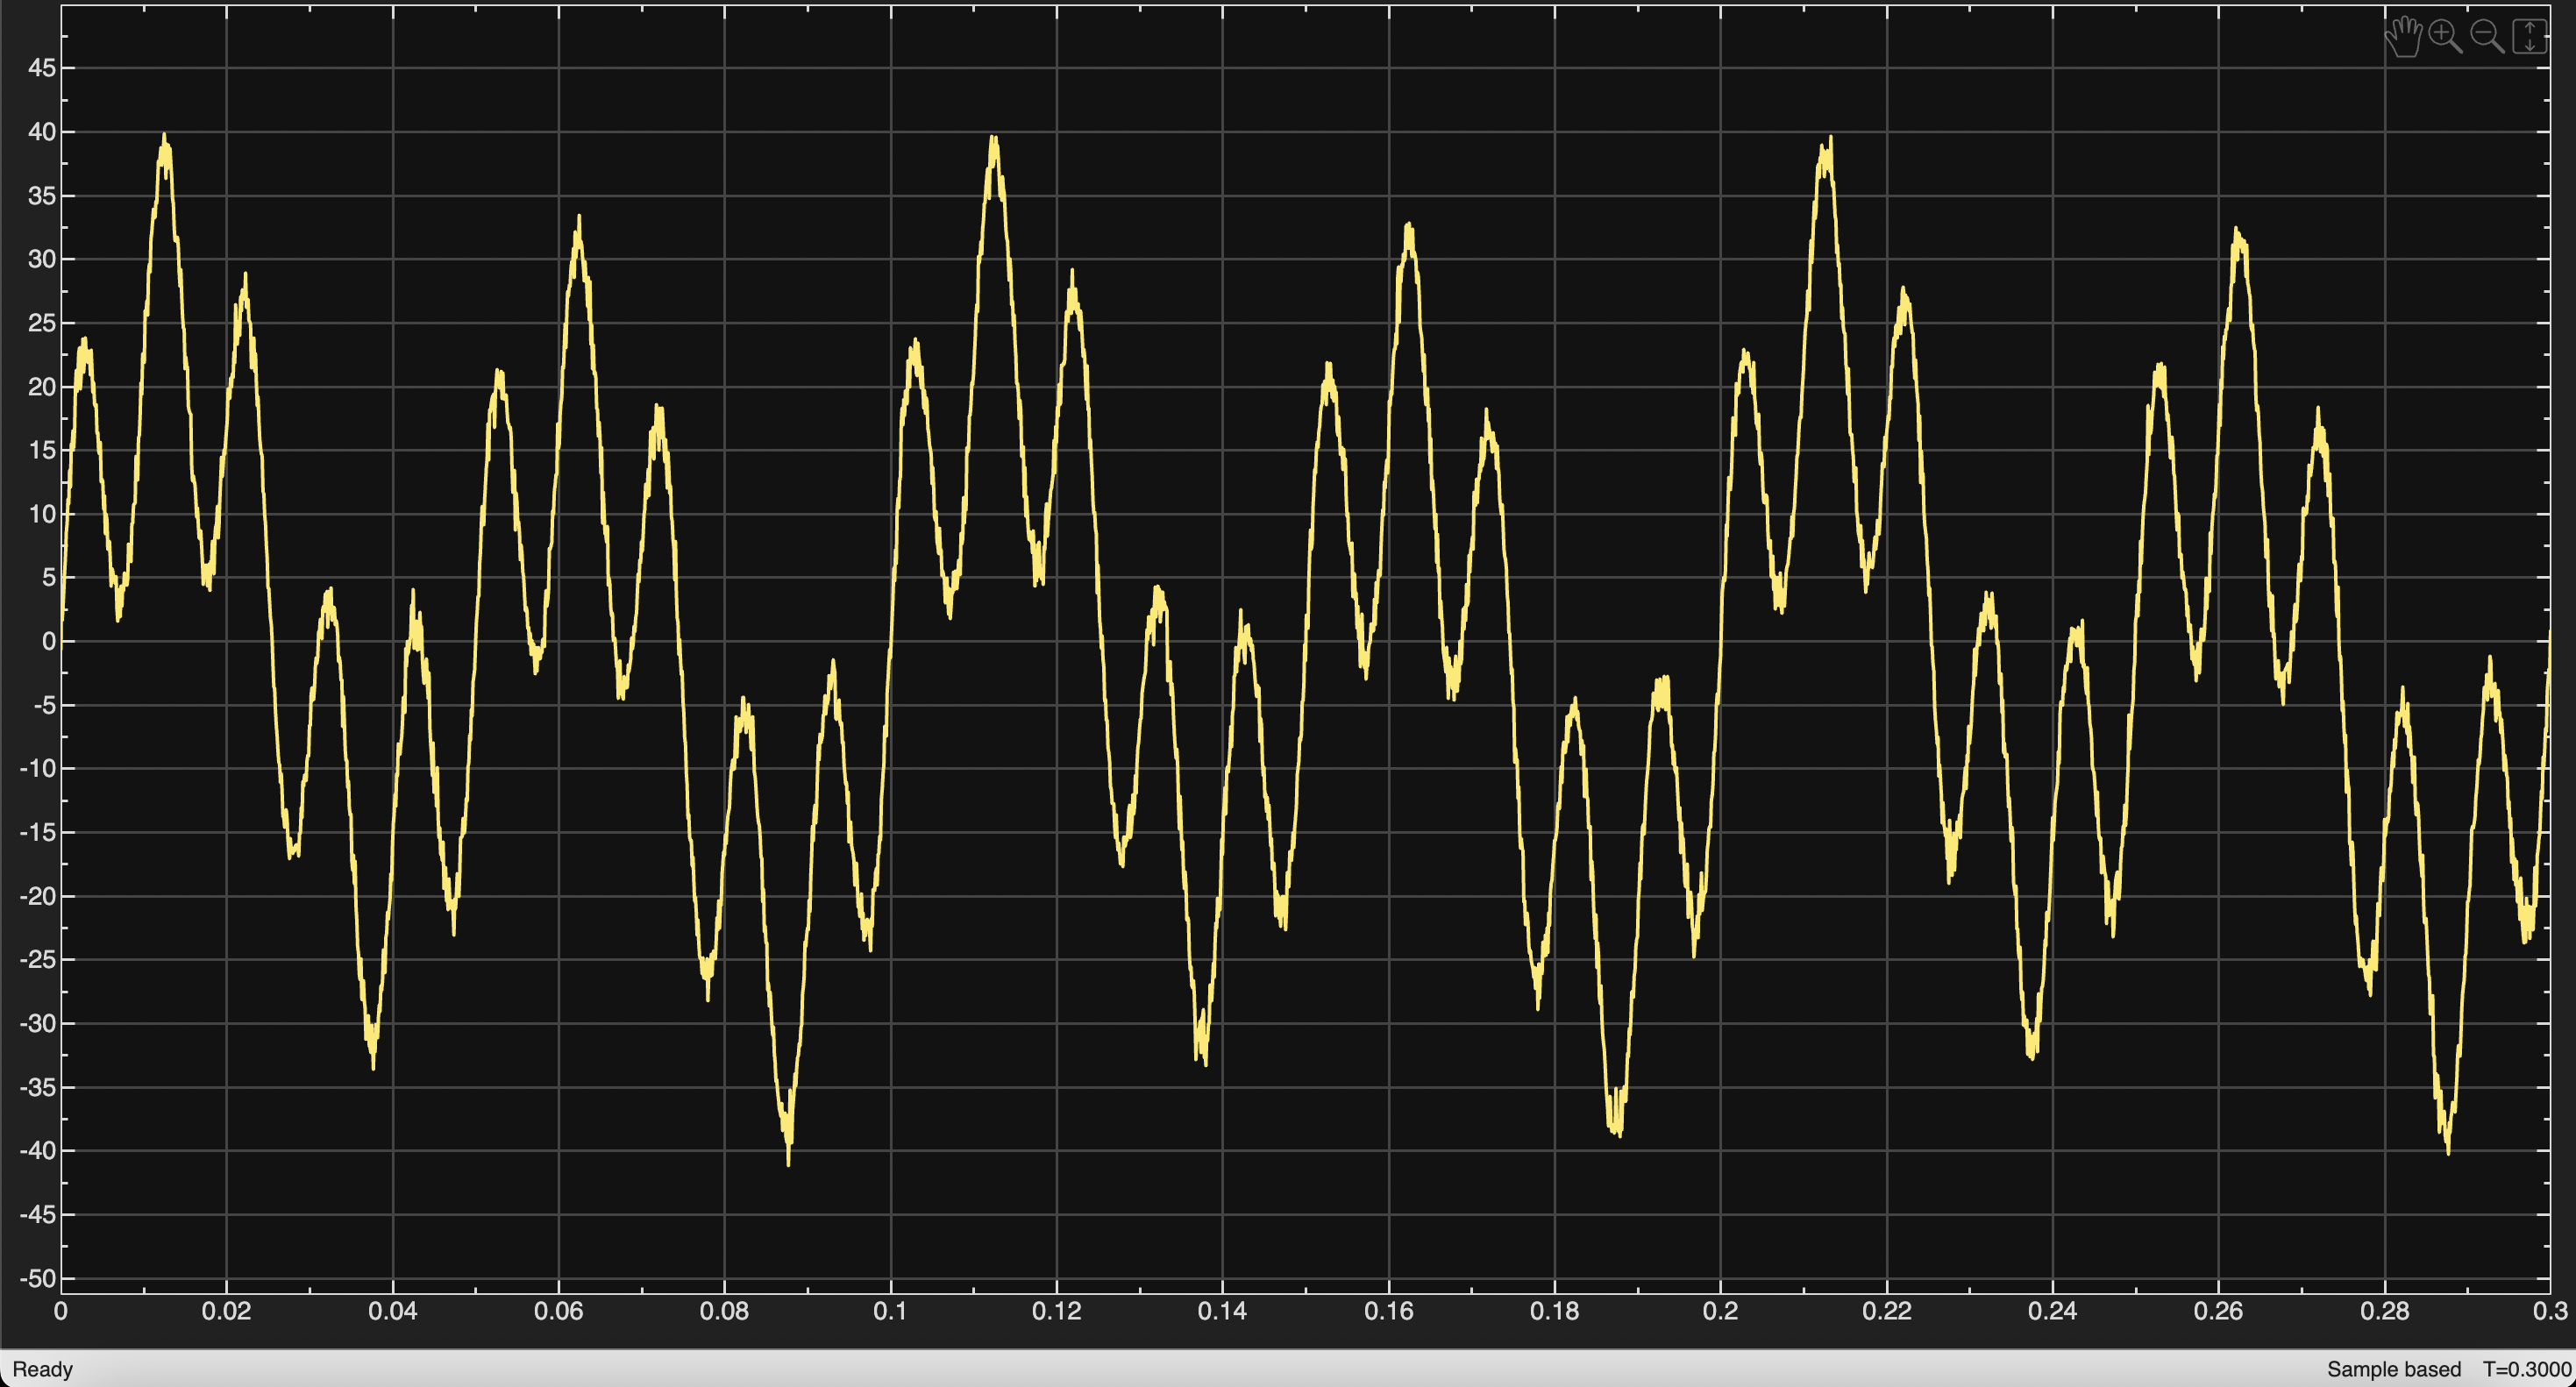
\includegraphics[width=\textwidth]{q2_5_rx_scope_gain_10_fc_100.png}
        \caption{Received, time domain.}
        \label{fig:q2-7-sum-rx-scope}
    \end{subfigure}
    \hfill
    \begin{subfigure}[b]{0.48\textwidth}
        \centering
        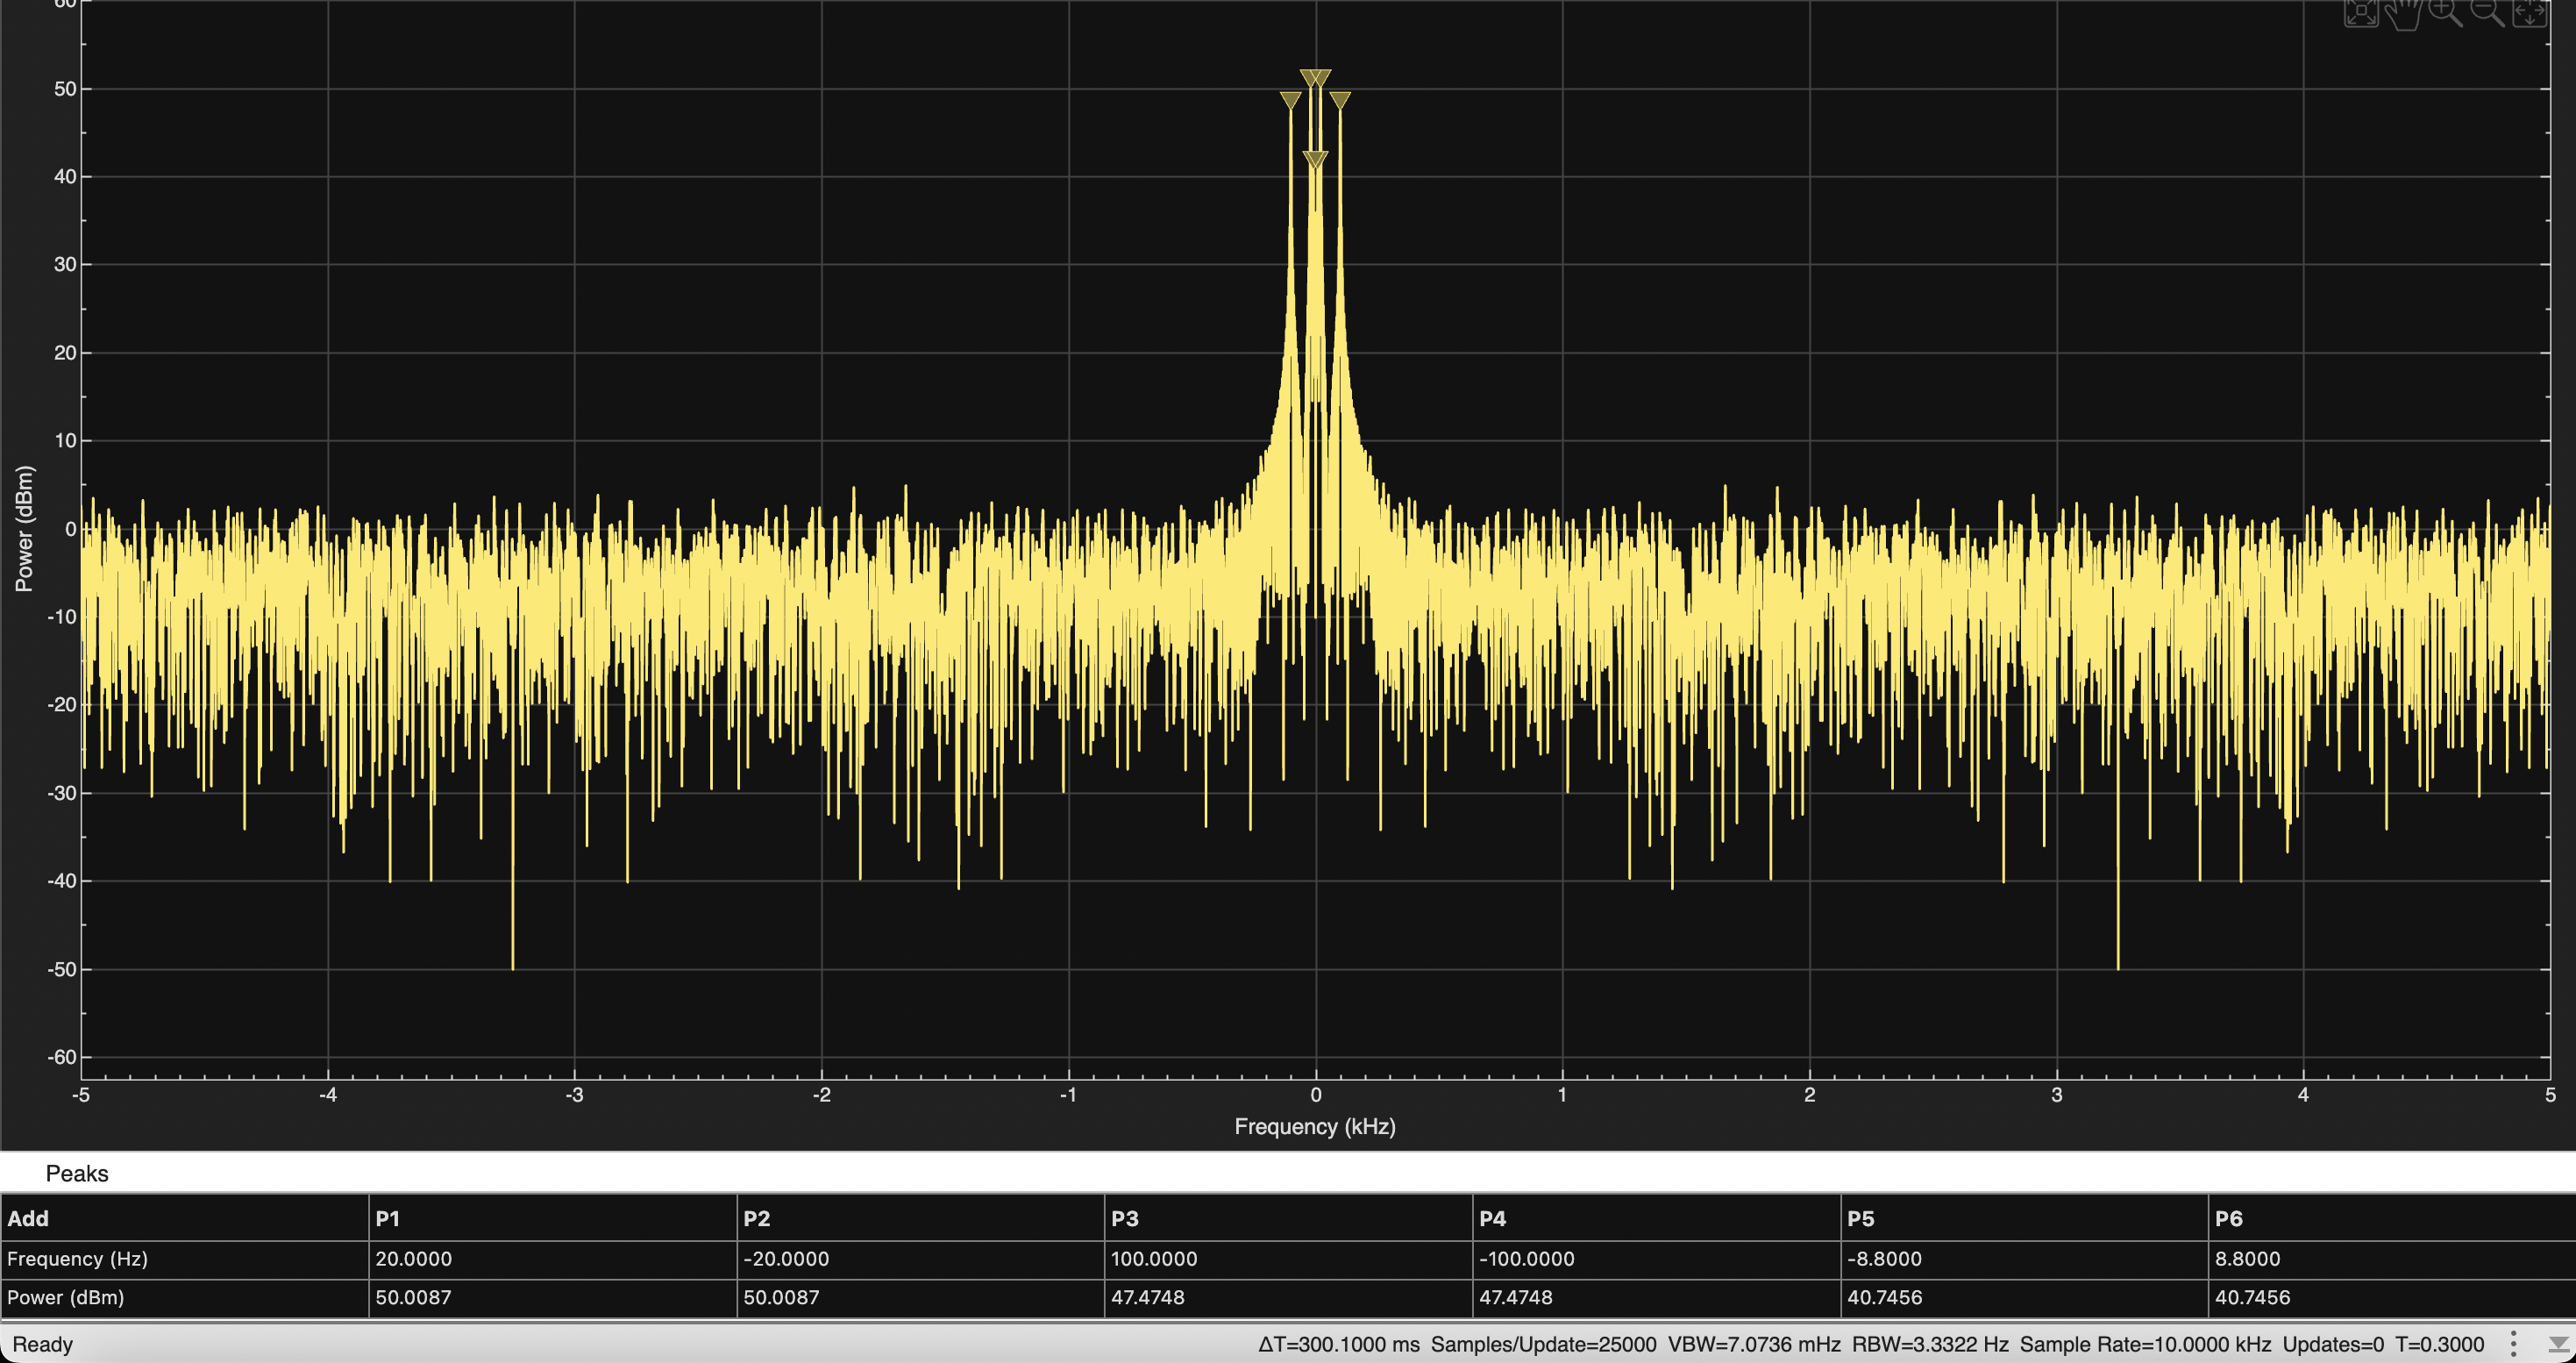
\includegraphics[width=\textwidth]{q2_5_rx_spectrum_gain_10_fc_100.png}
        \caption{Received, spectrum.}
        \label{fig:q2-7-sum-rx-spectrum}
    \end{subfigure}

    \vspace{0.6em}

    \begin{subfigure}[b]{0.48\textwidth}
        \centering
        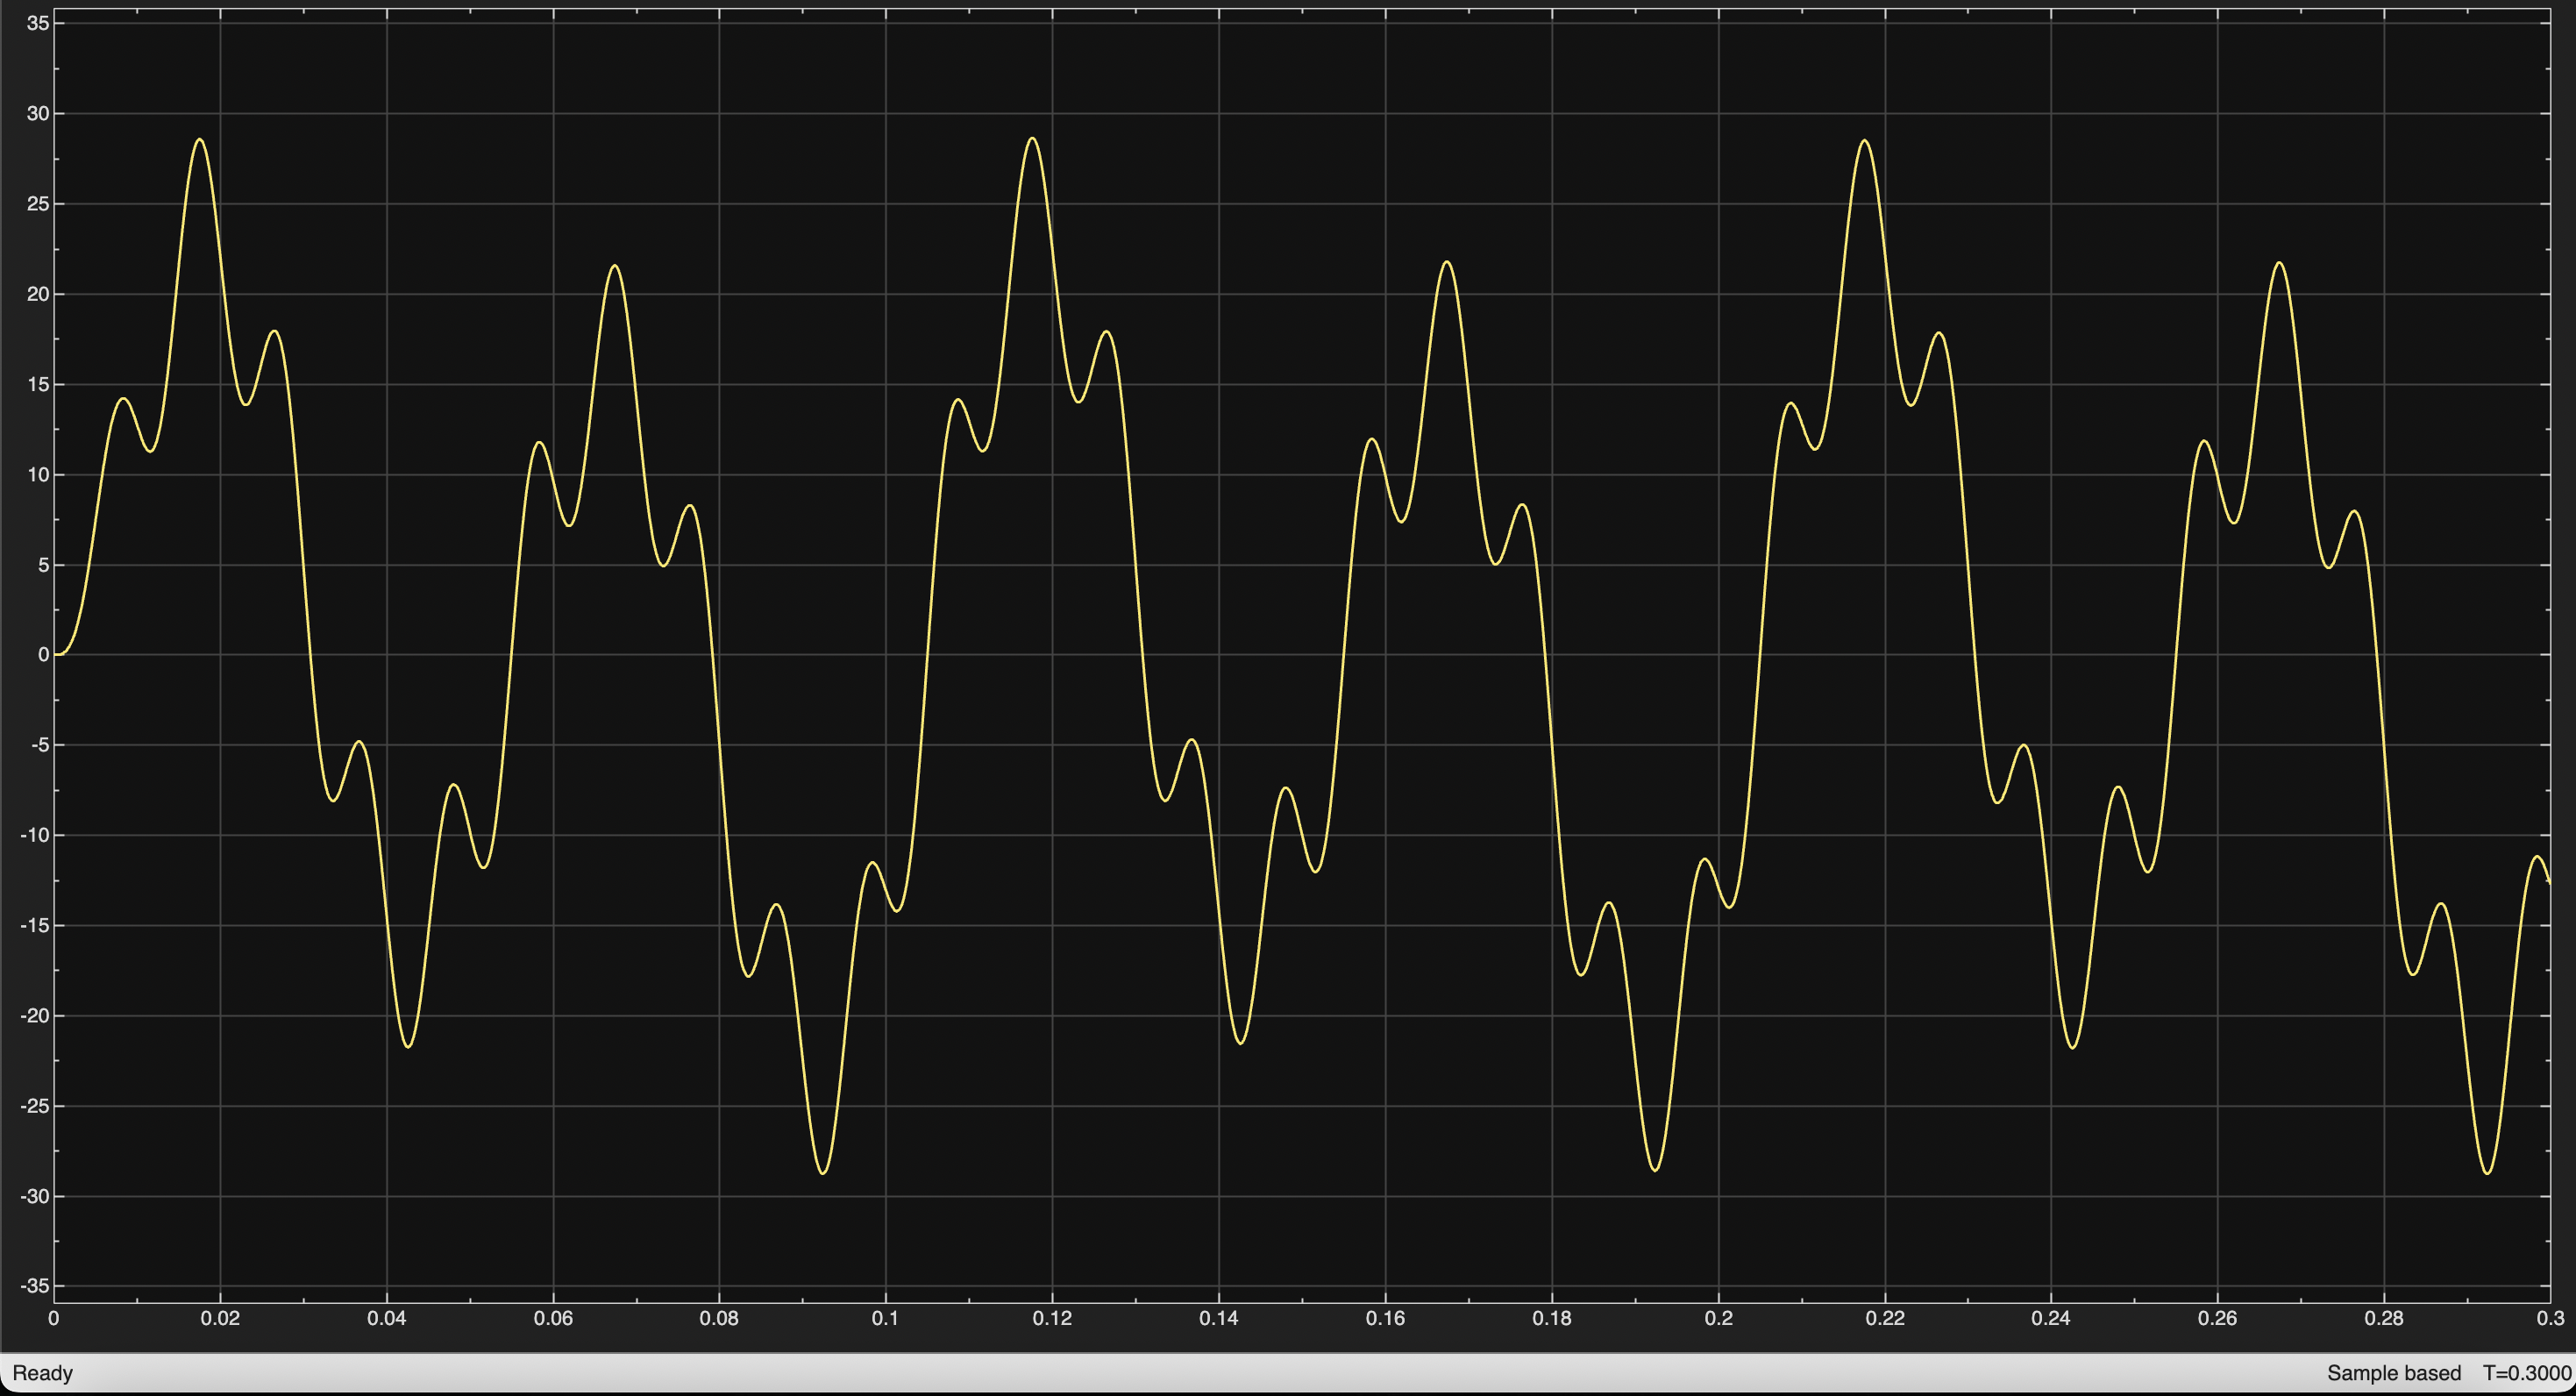
\includegraphics[width=\textwidth]{q2_5_filtered_scope_gain_10_fc_100.png}
        \caption{Filtered, time domain.}
        \label{fig:q2-5-filtered-scope}
    \end{subfigure}
    \hfill
    \begin{subfigure}[b]{0.48\textwidth}
        \centering
        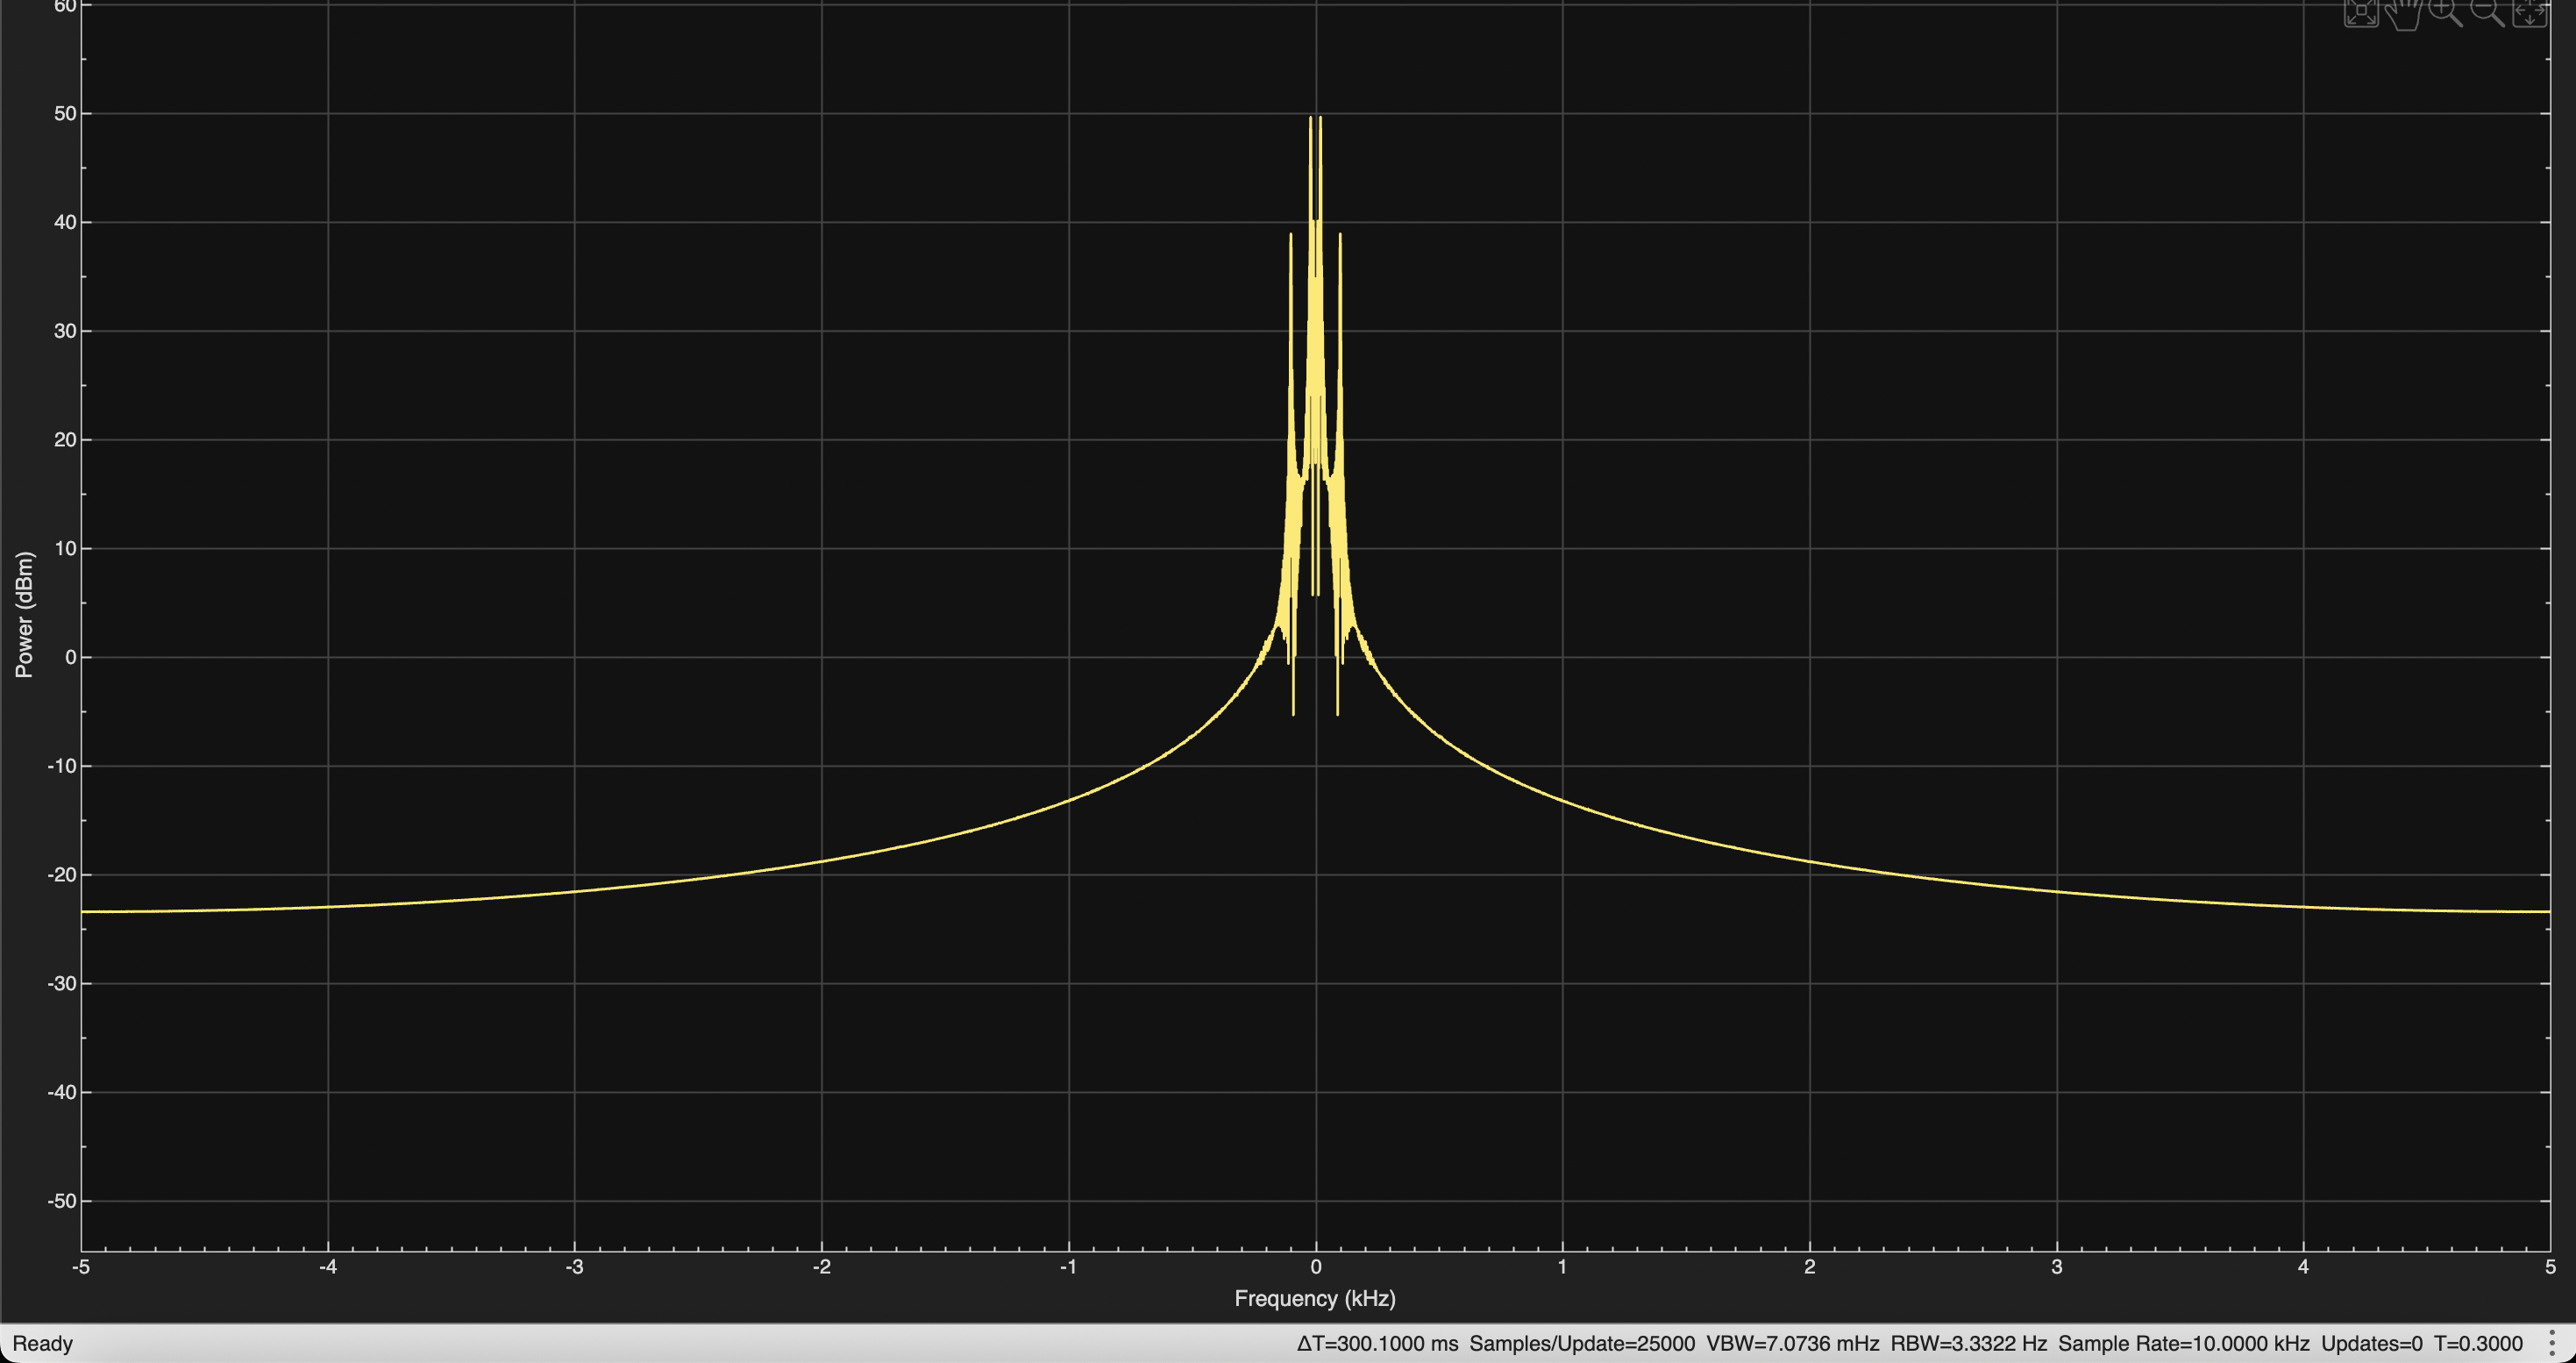
\includegraphics[width=\textwidth]{q2_5_filtered_spectrum_gain_10_fc_100.png}
        \caption{Filtered, spectrum.}
        \label{fig:q2-5-filtered-spectrum}
    \end{subfigure}
    \caption{Sum of three sine waves before filtering (top) and after filtering (bottom), at Slider Gain 10 and $F_c=100$\,Hz.}
    \label{fig:q2-7-sum-comparison}
\end{figure}

\subsection*{Question 8}

With the results below, we can observe the following:
\begin{itemize}
    \item Increasing the signal gain means a higher SNR. A higher SNR means that the noise has less of an effect on the resulting signal, so the
    filtered signal appears to be less and less noisy (even though the noise itself hasn't changed). This also continues into the frequency domain, where the spectral graph is smoother with higher SNR.
    \item Increasing the cutoff frequency means that more noise is kept in the resulting signal. This basically means a lower SNR, which implies a noisier signal. A noisier signal also means
    that the frequency domain graph has a larger and larger bandwidth of just noise, which ends up making the time-domain graph noisier.
\end{itemize}

\subsubsection*{Baseline: gain 10, $F_c=100$\,Hz}

\begin{figure}[H]
    \centering
    \begin{subfigure}[b]{0.48\textwidth}
        \centering
        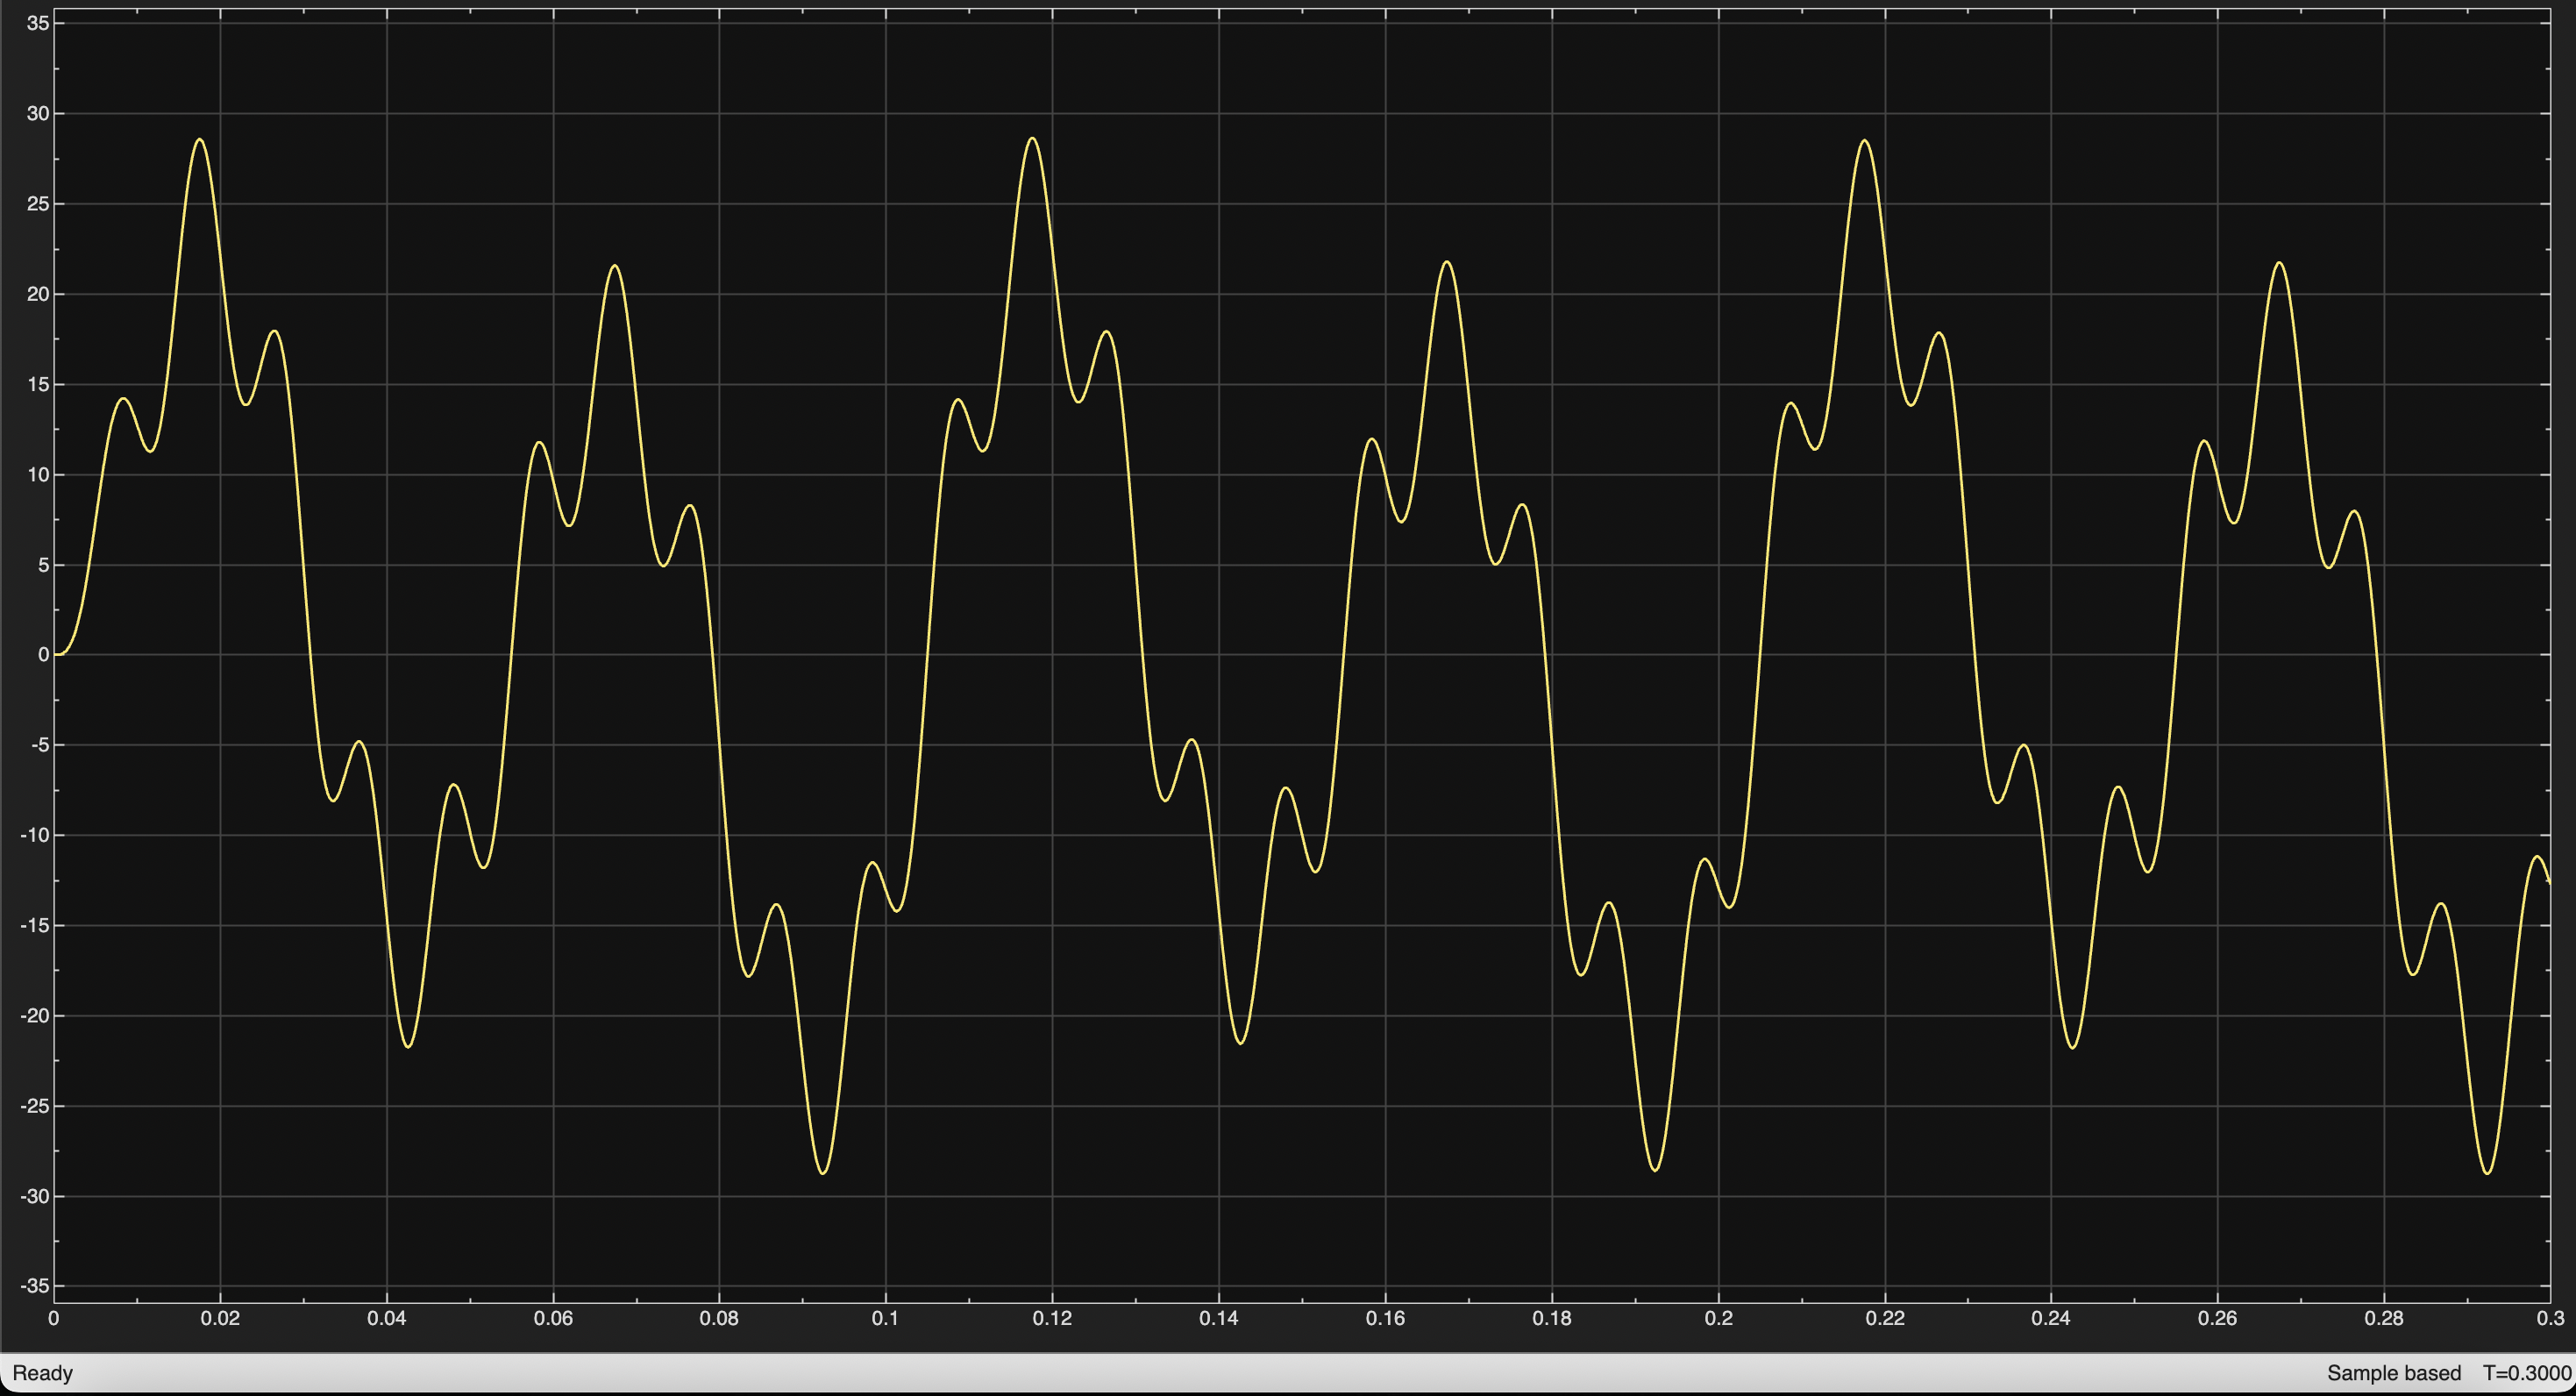
\includegraphics[width=\linewidth]{q2_5_filtered_scope_gain_10_fc_100.png}
        \caption{Time domain.}
    \end{subfigure}
    \hfill
    \begin{subfigure}[b]{0.48\textwidth}
        \centering
        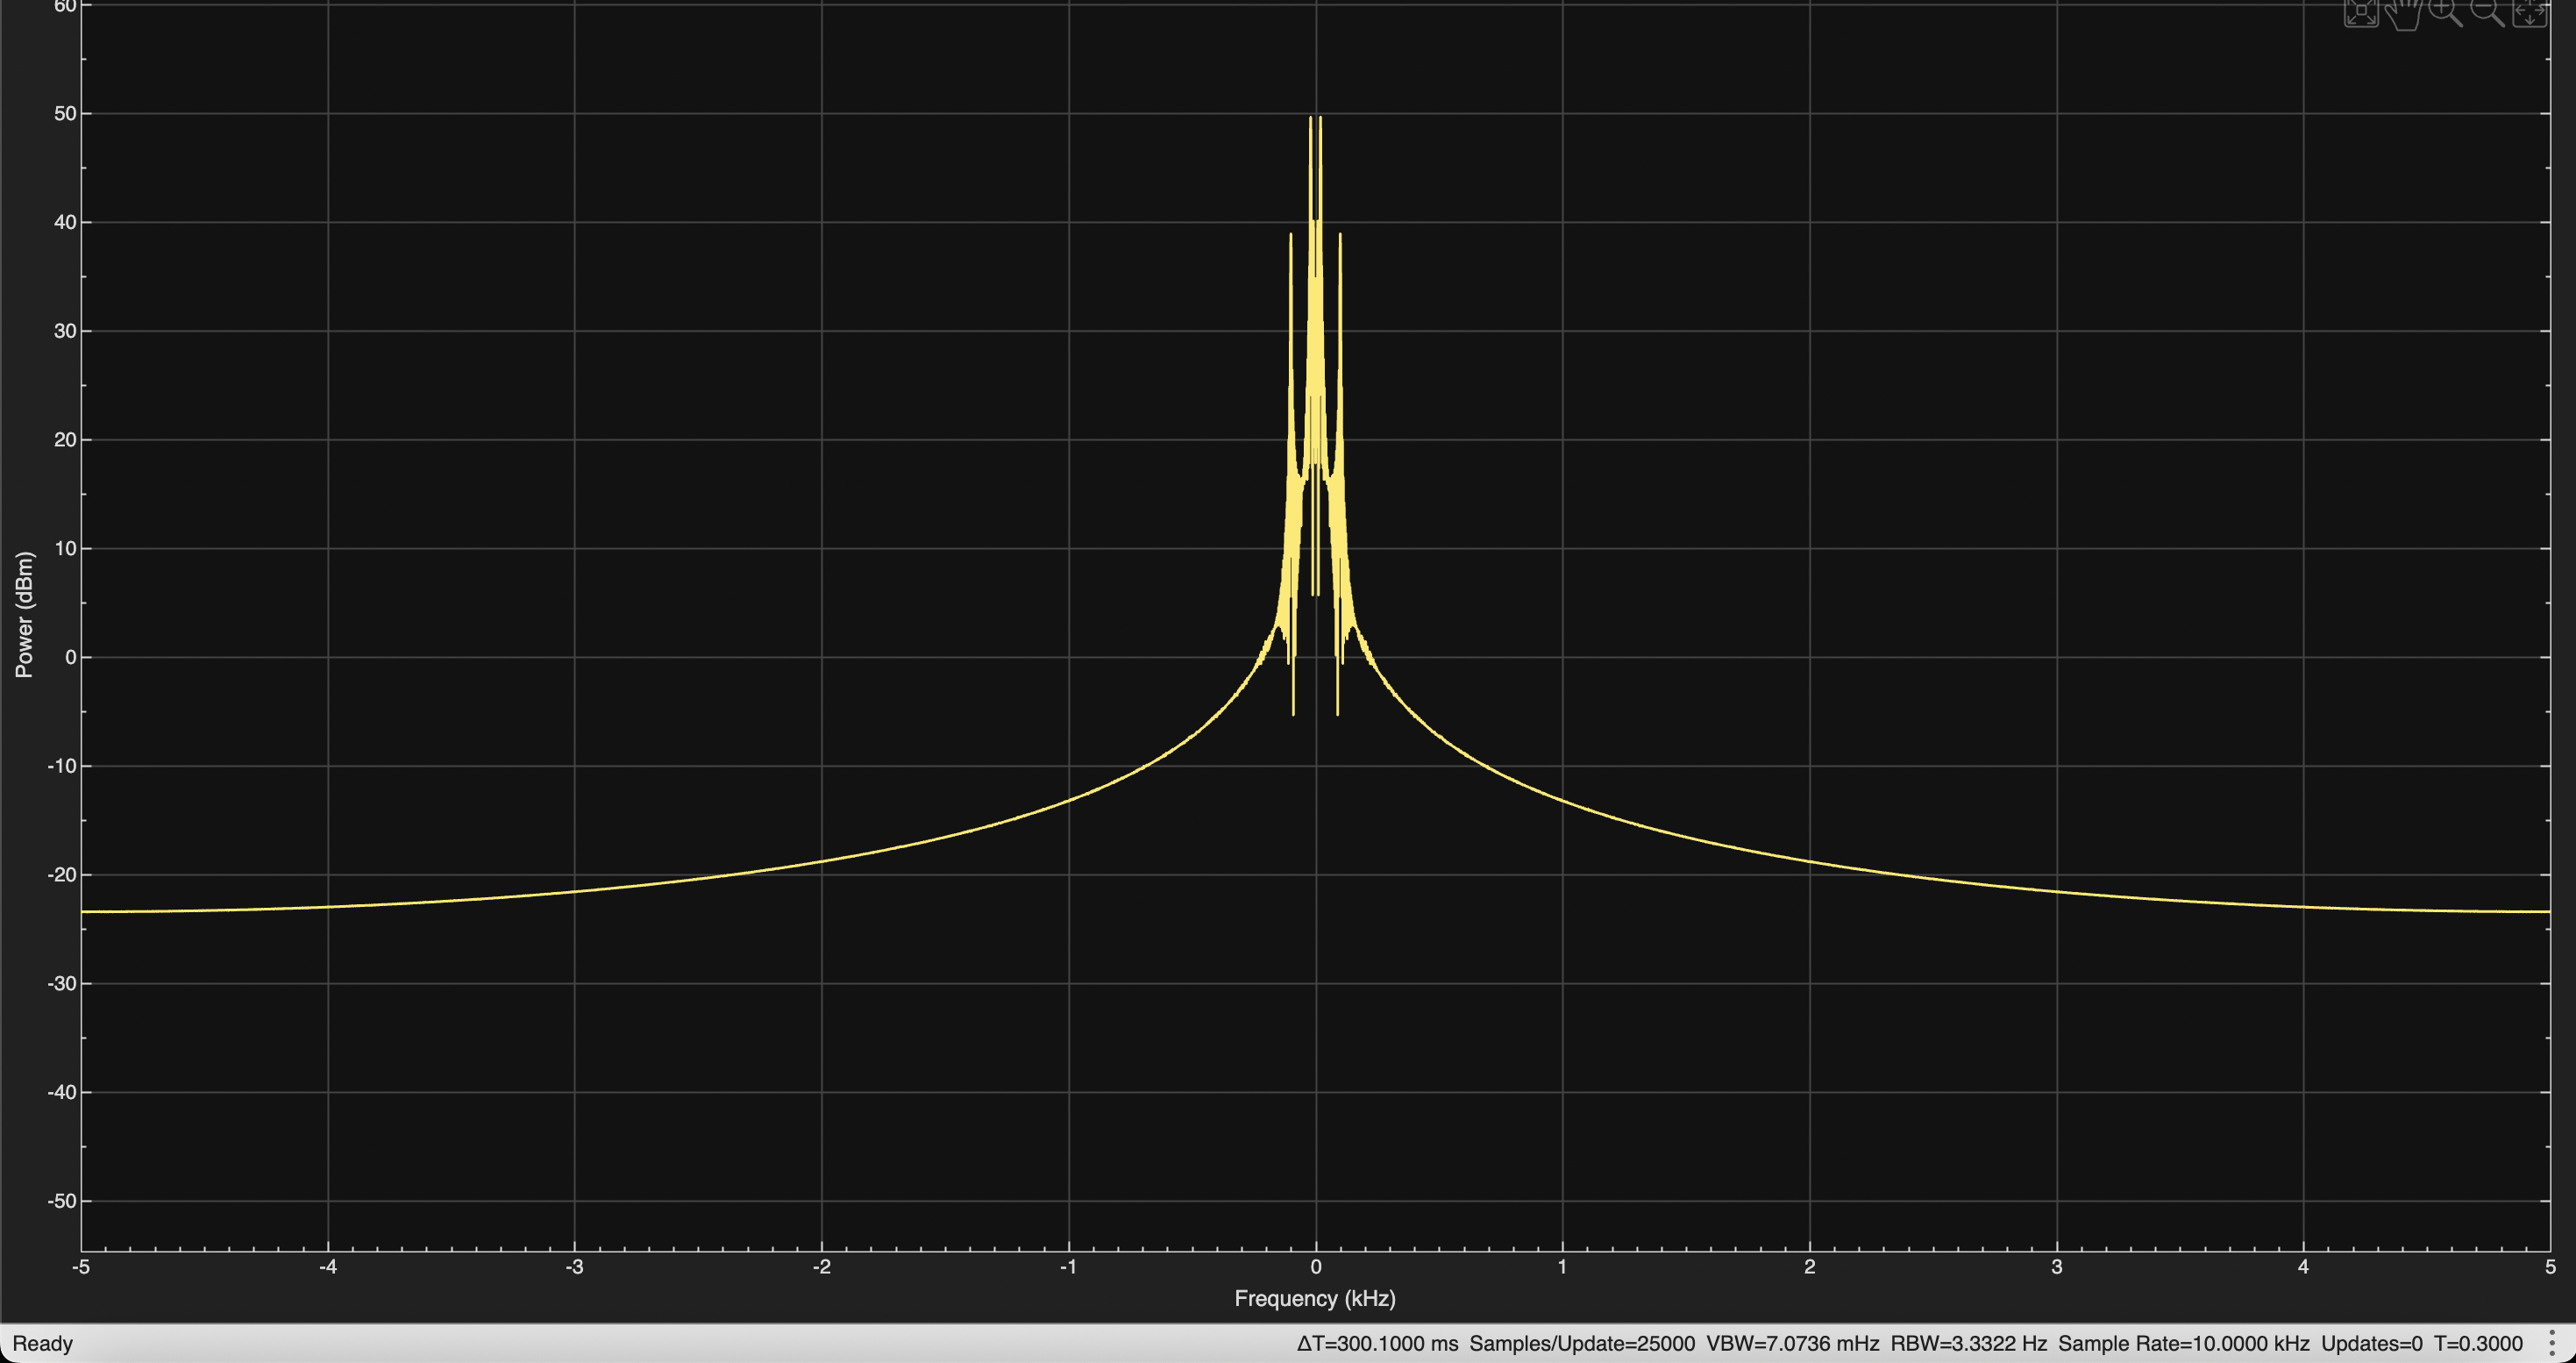
\includegraphics[width=\linewidth]{q2_5_filtered_spectrum_gain_10_fc_100.png}
        \caption{Spectrum.}
    \end{subfigure}
    \caption{Baseline: filtered sum of three sine waves at gain 10 and $F_c=100$\,Hz.}
    \label{fig:q2-8-gain-10-fc-100}
\end{figure}

\subsubsection*{Varying the gain ($F_c=100$\,Hz)}

\begin{figure}[H]
    \centering
    \begin{subfigure}[b]{0.48\textwidth}
        \centering
        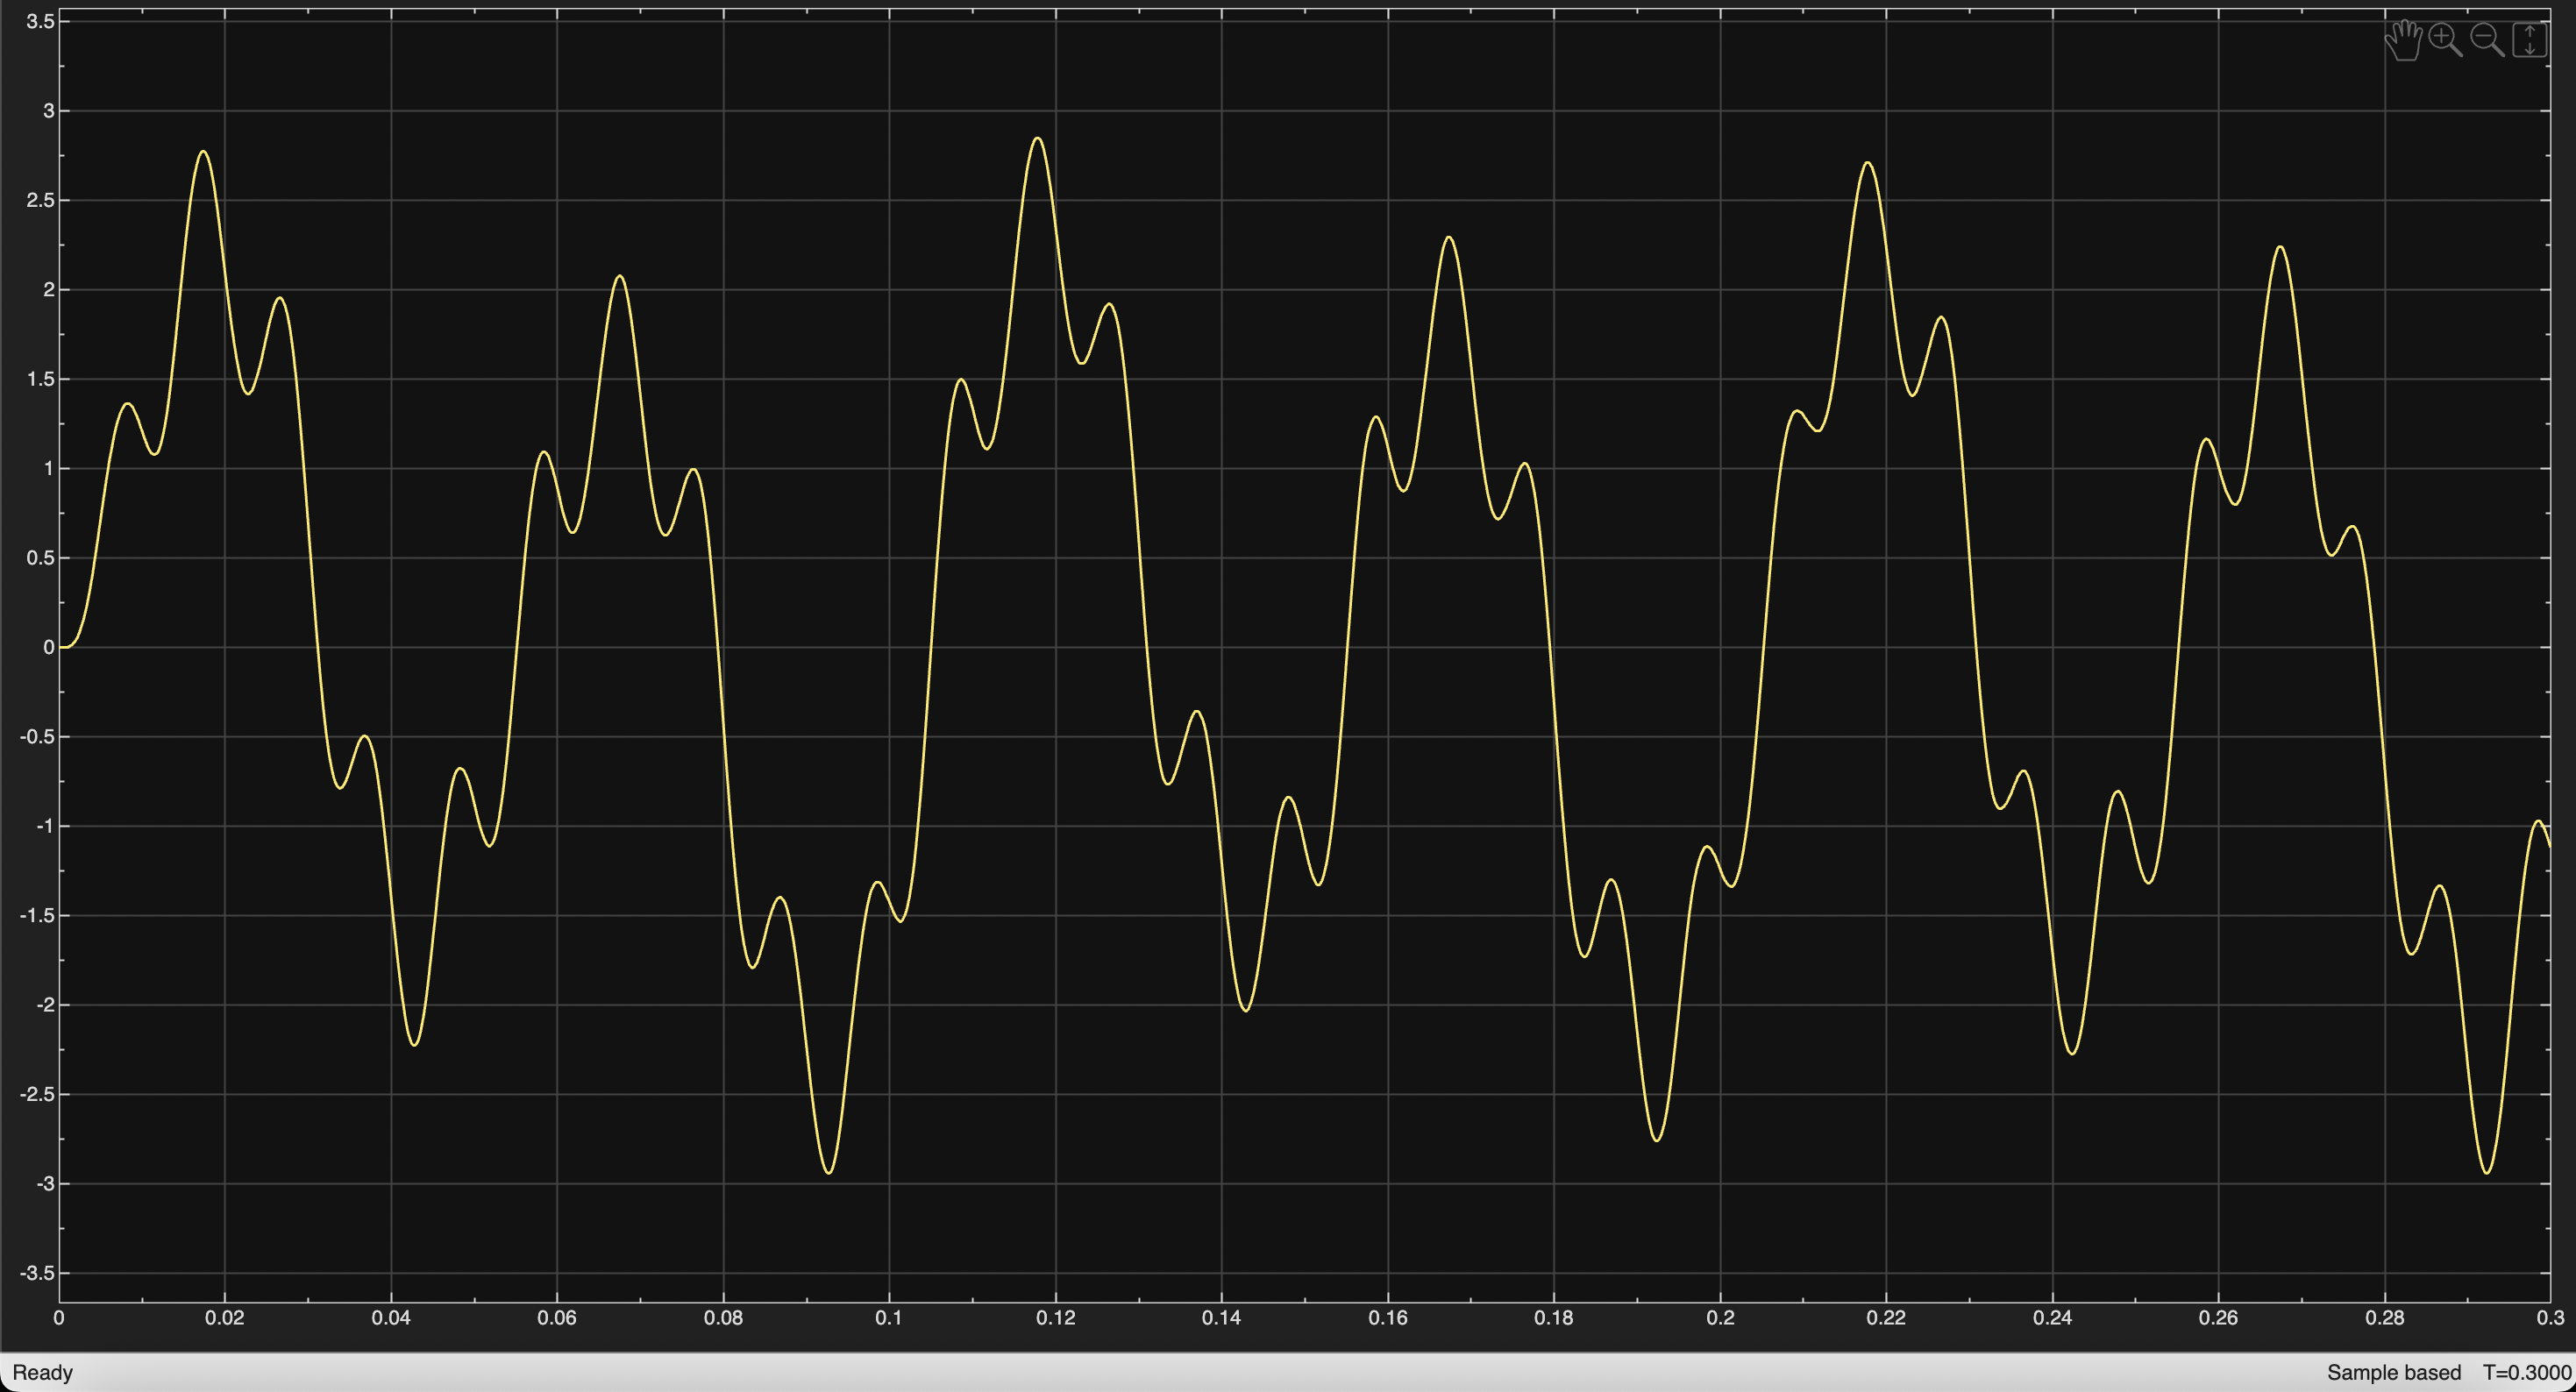
\includegraphics[width=\linewidth]{q2_5_filtered_scope_gain_1_fc_100.png}
        \caption{Time domain.}
    \end{subfigure}
    \hfill
    \begin{subfigure}[b]{0.48\textwidth}
        \centering
        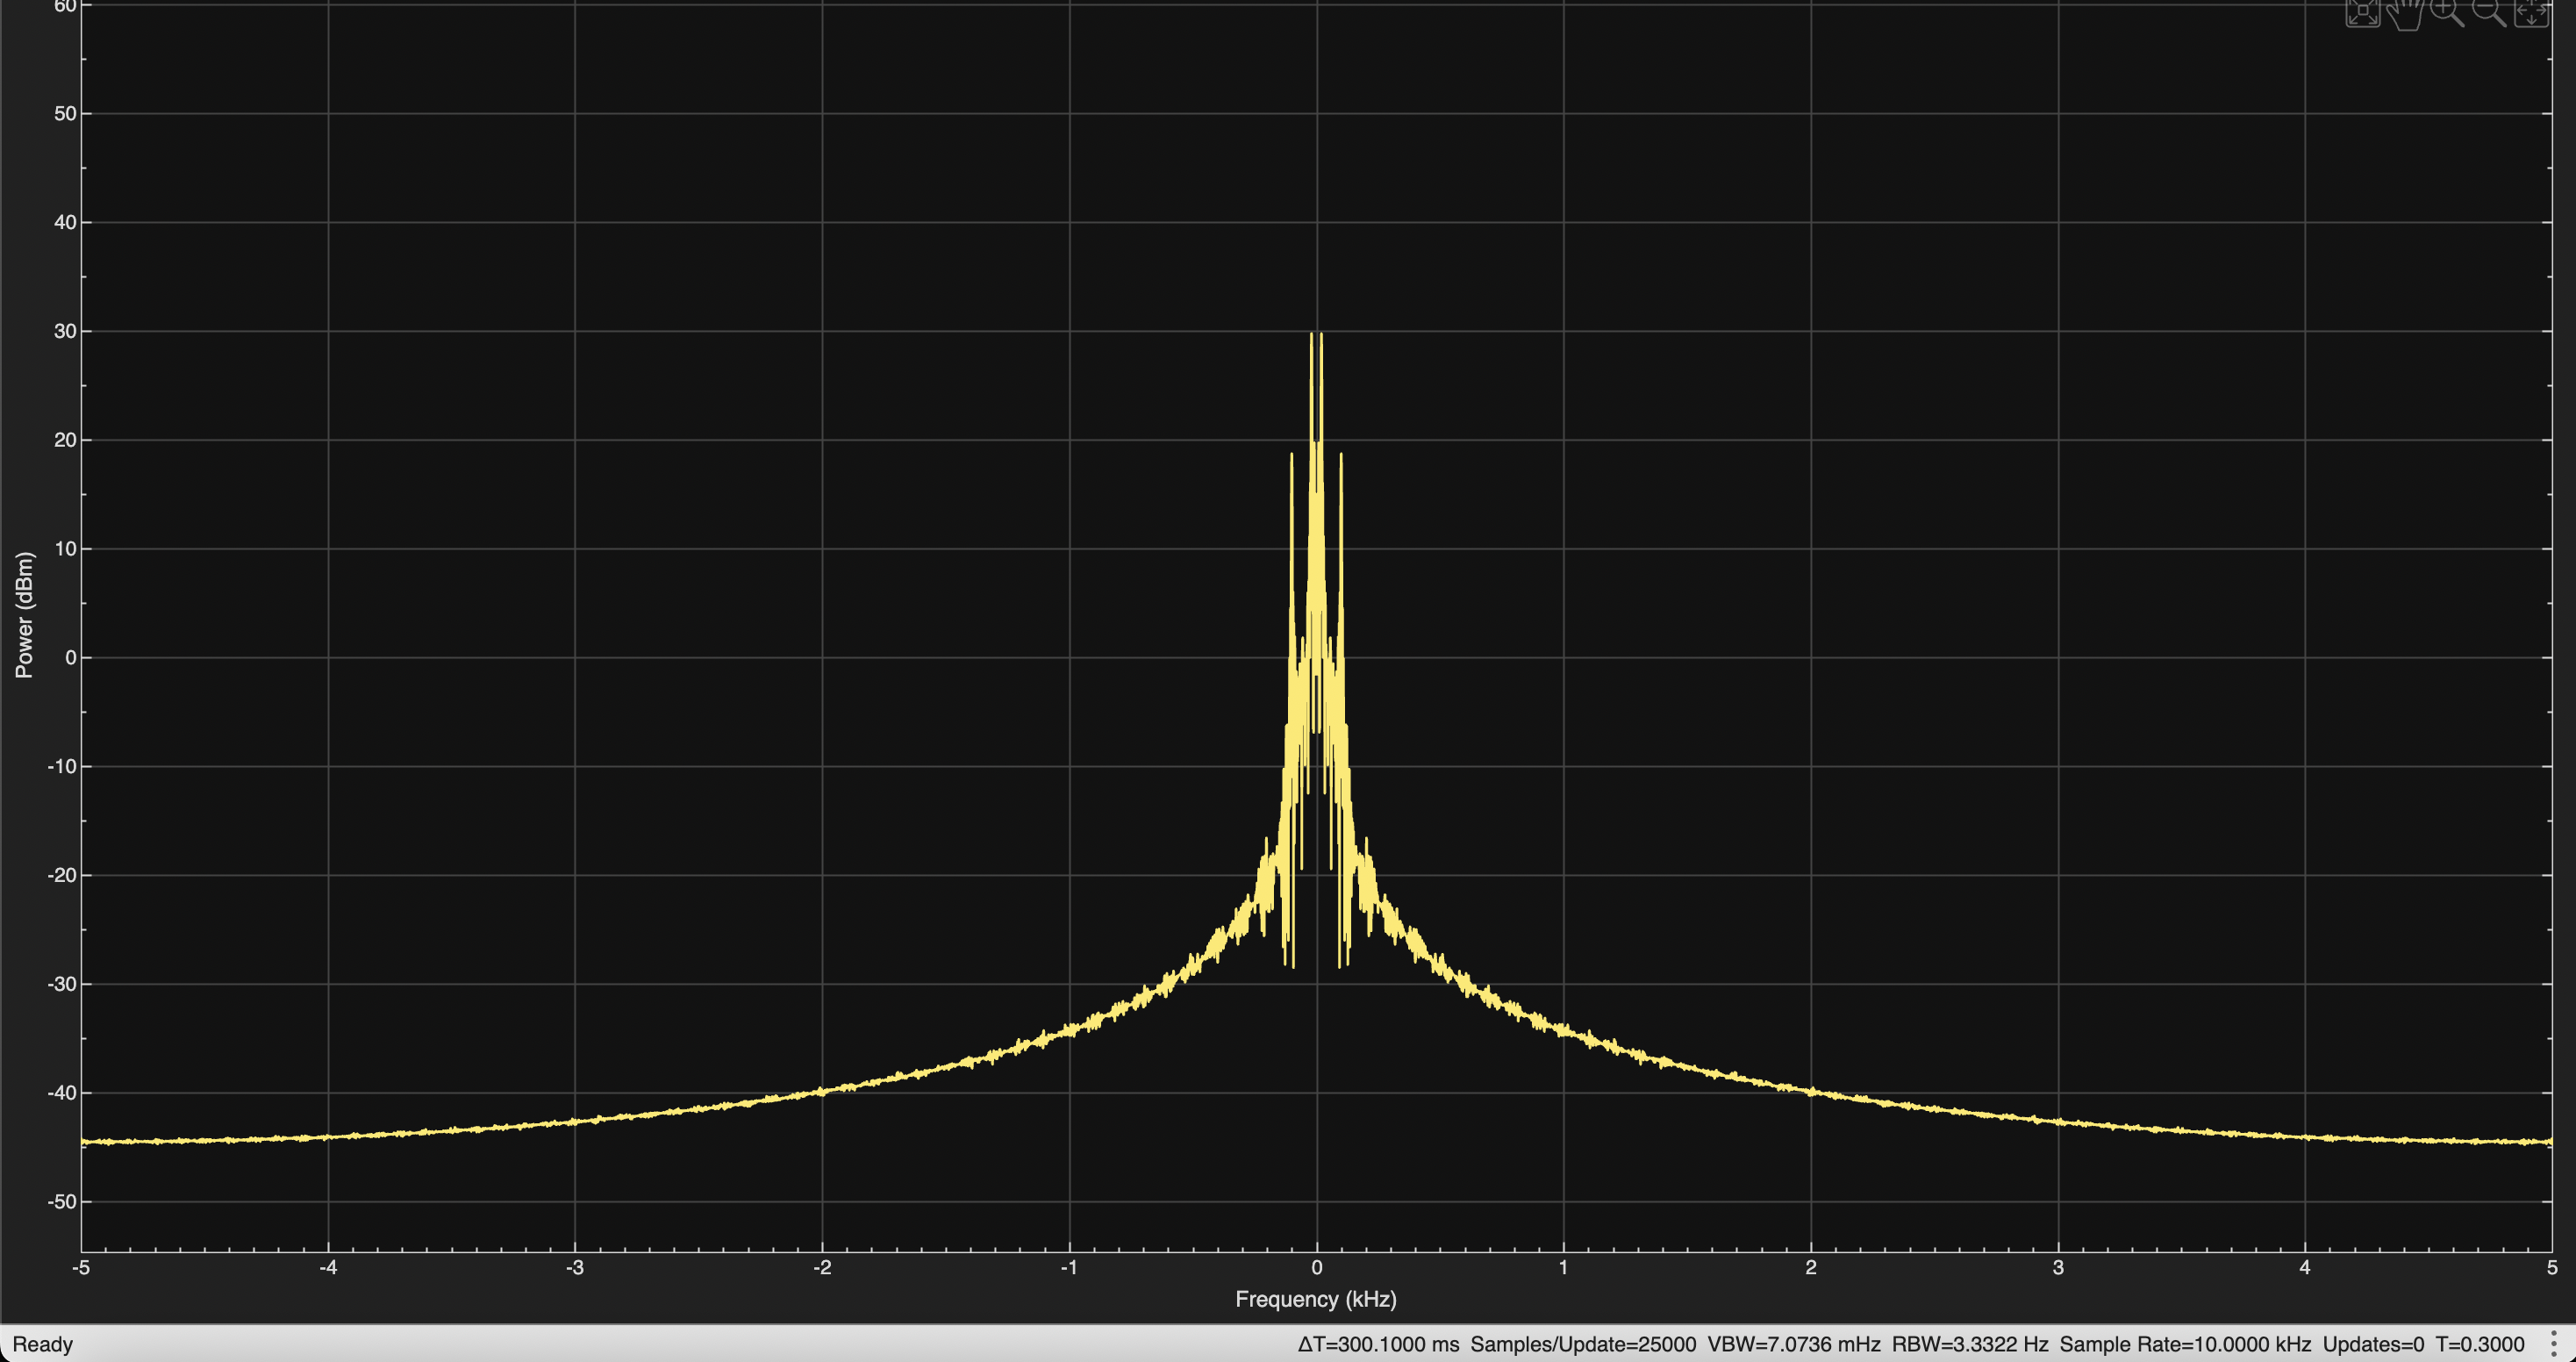
\includegraphics[width=\linewidth]{q2_5_filtered_spectrum_gain_1_fc_100.png}
        \caption{Spectrum.}
    \end{subfigure}
    \caption{Lower gain: filtered sum of three sine waves at gain 1 and $F_c=100$\,Hz.}
    \label{fig:q2-8-gain-1-fc-100}
\end{figure}

\begin{figure}[H]
    \centering
    \begin{subfigure}[b]{0.48\textwidth}
        \centering
        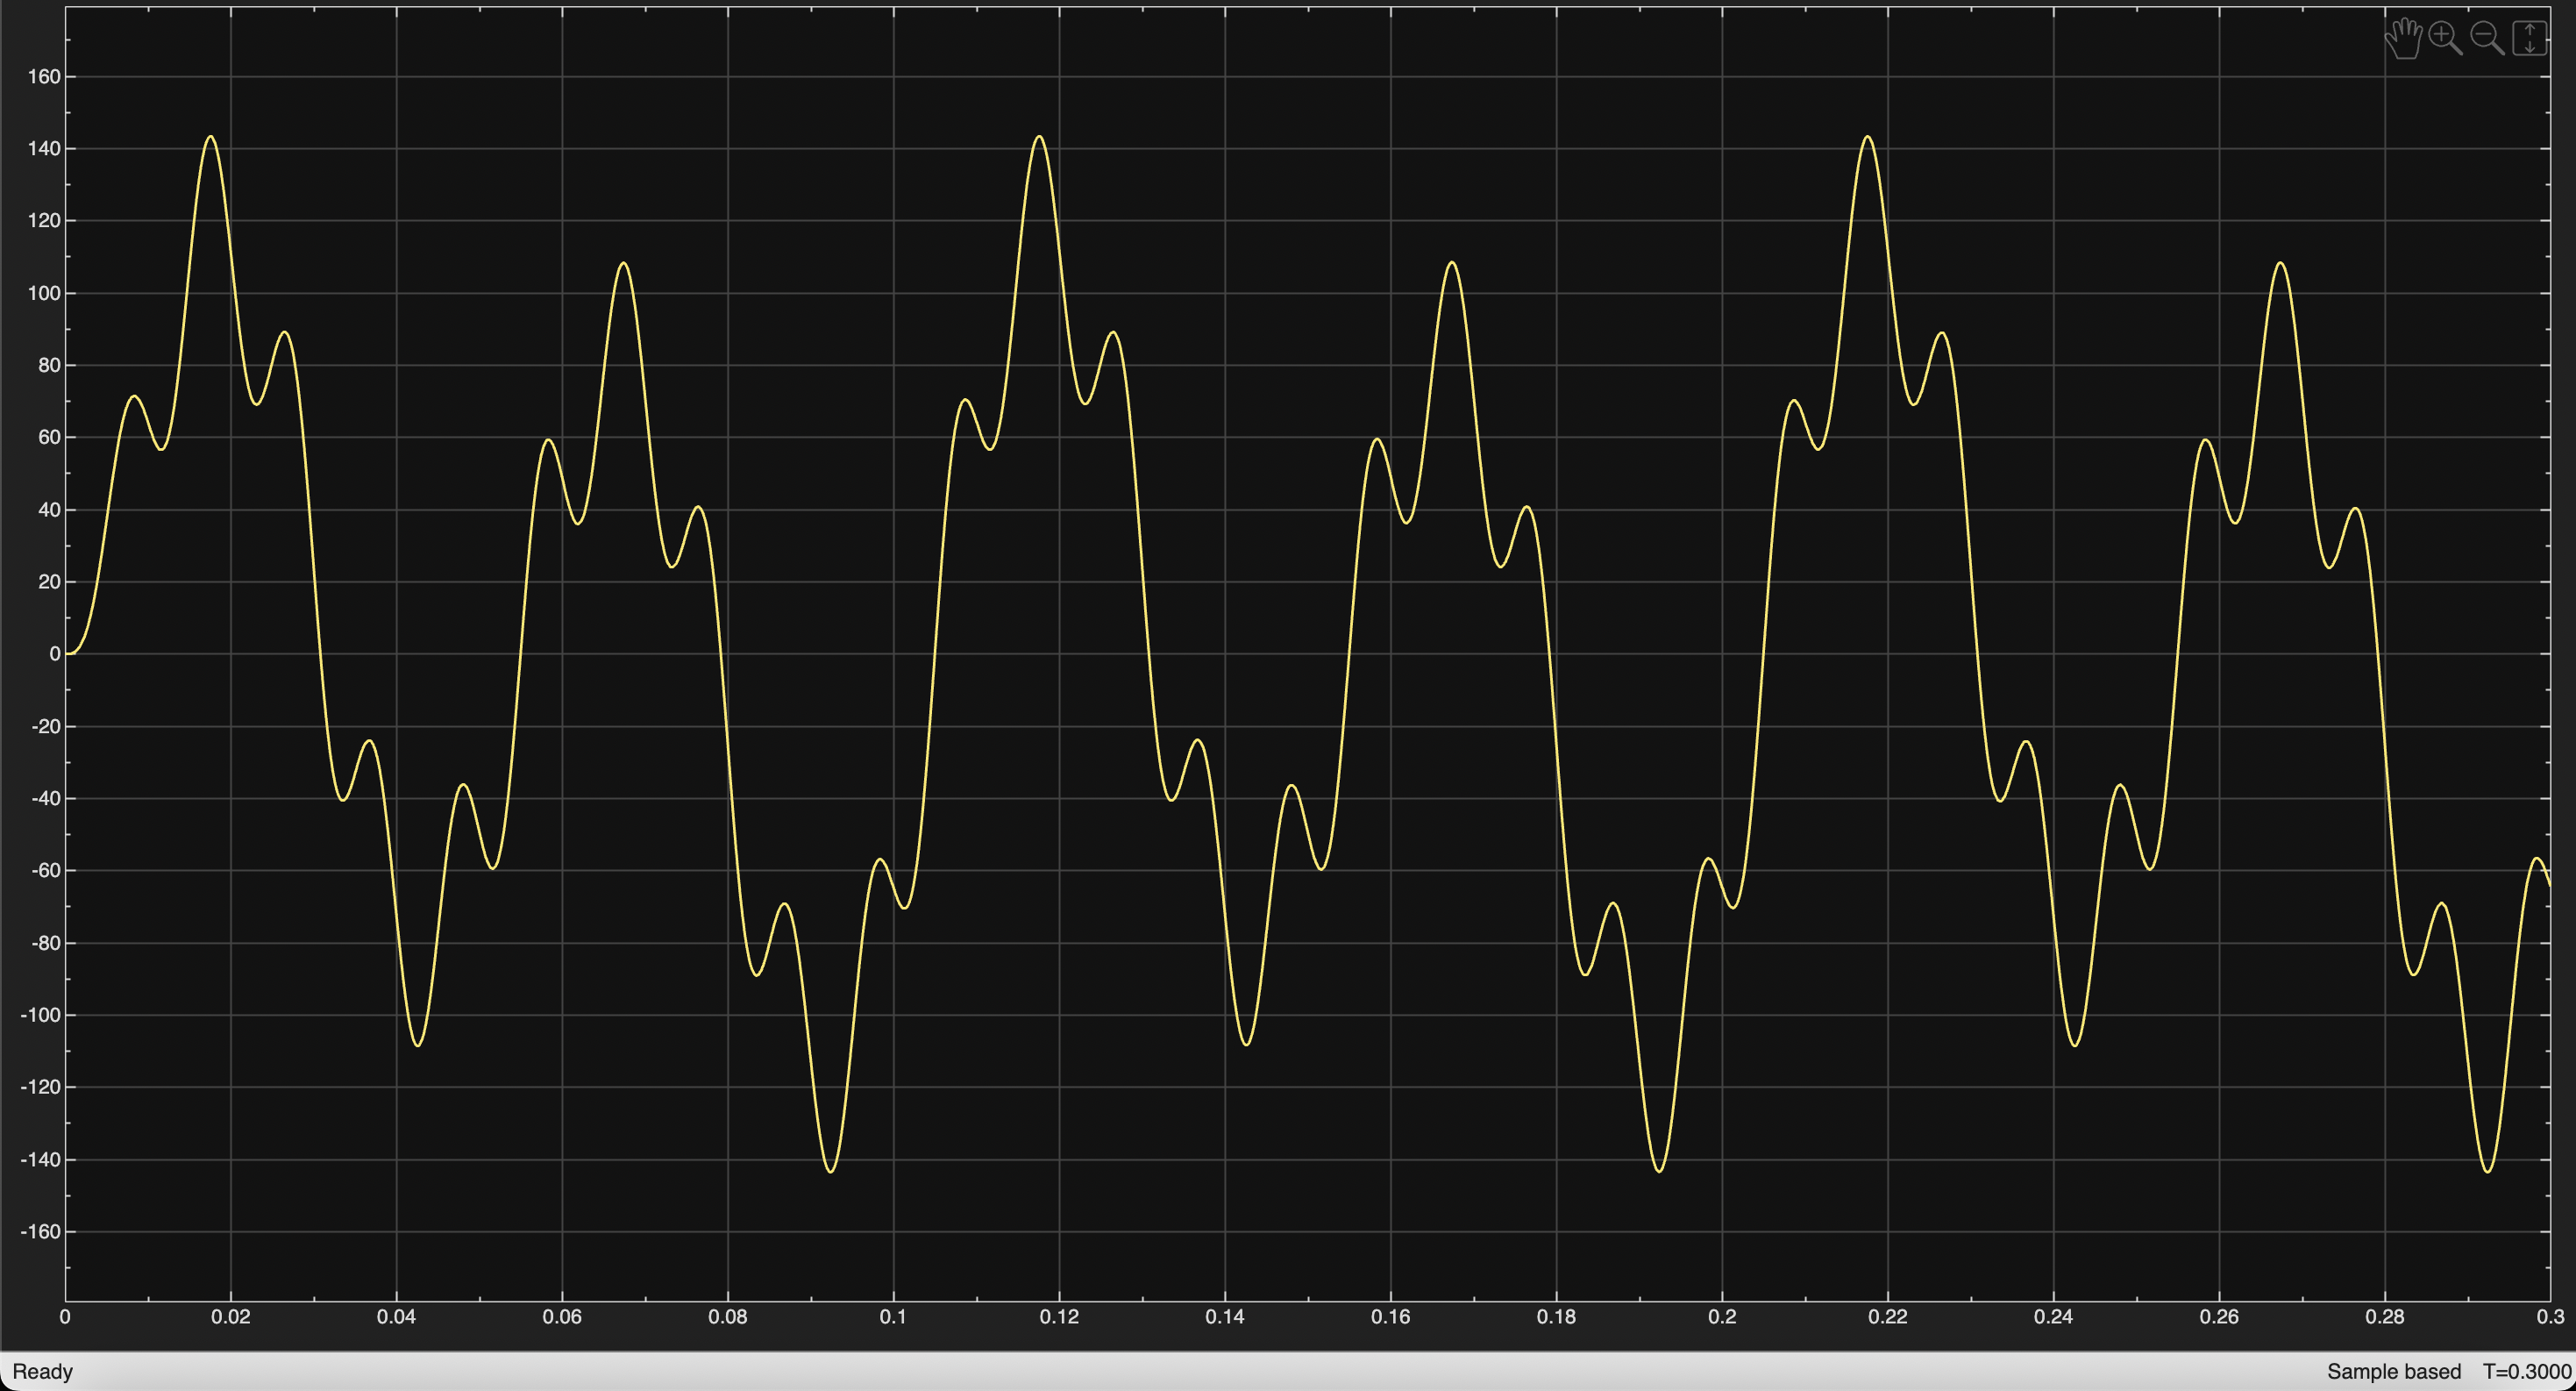
\includegraphics[width=\linewidth]{q2_5_filtered_scope_gain_50_fc_100.png}
        \caption{Time domain.}
    \end{subfigure}
    \hfill
    \begin{subfigure}[b]{0.48\textwidth}
        \centering
        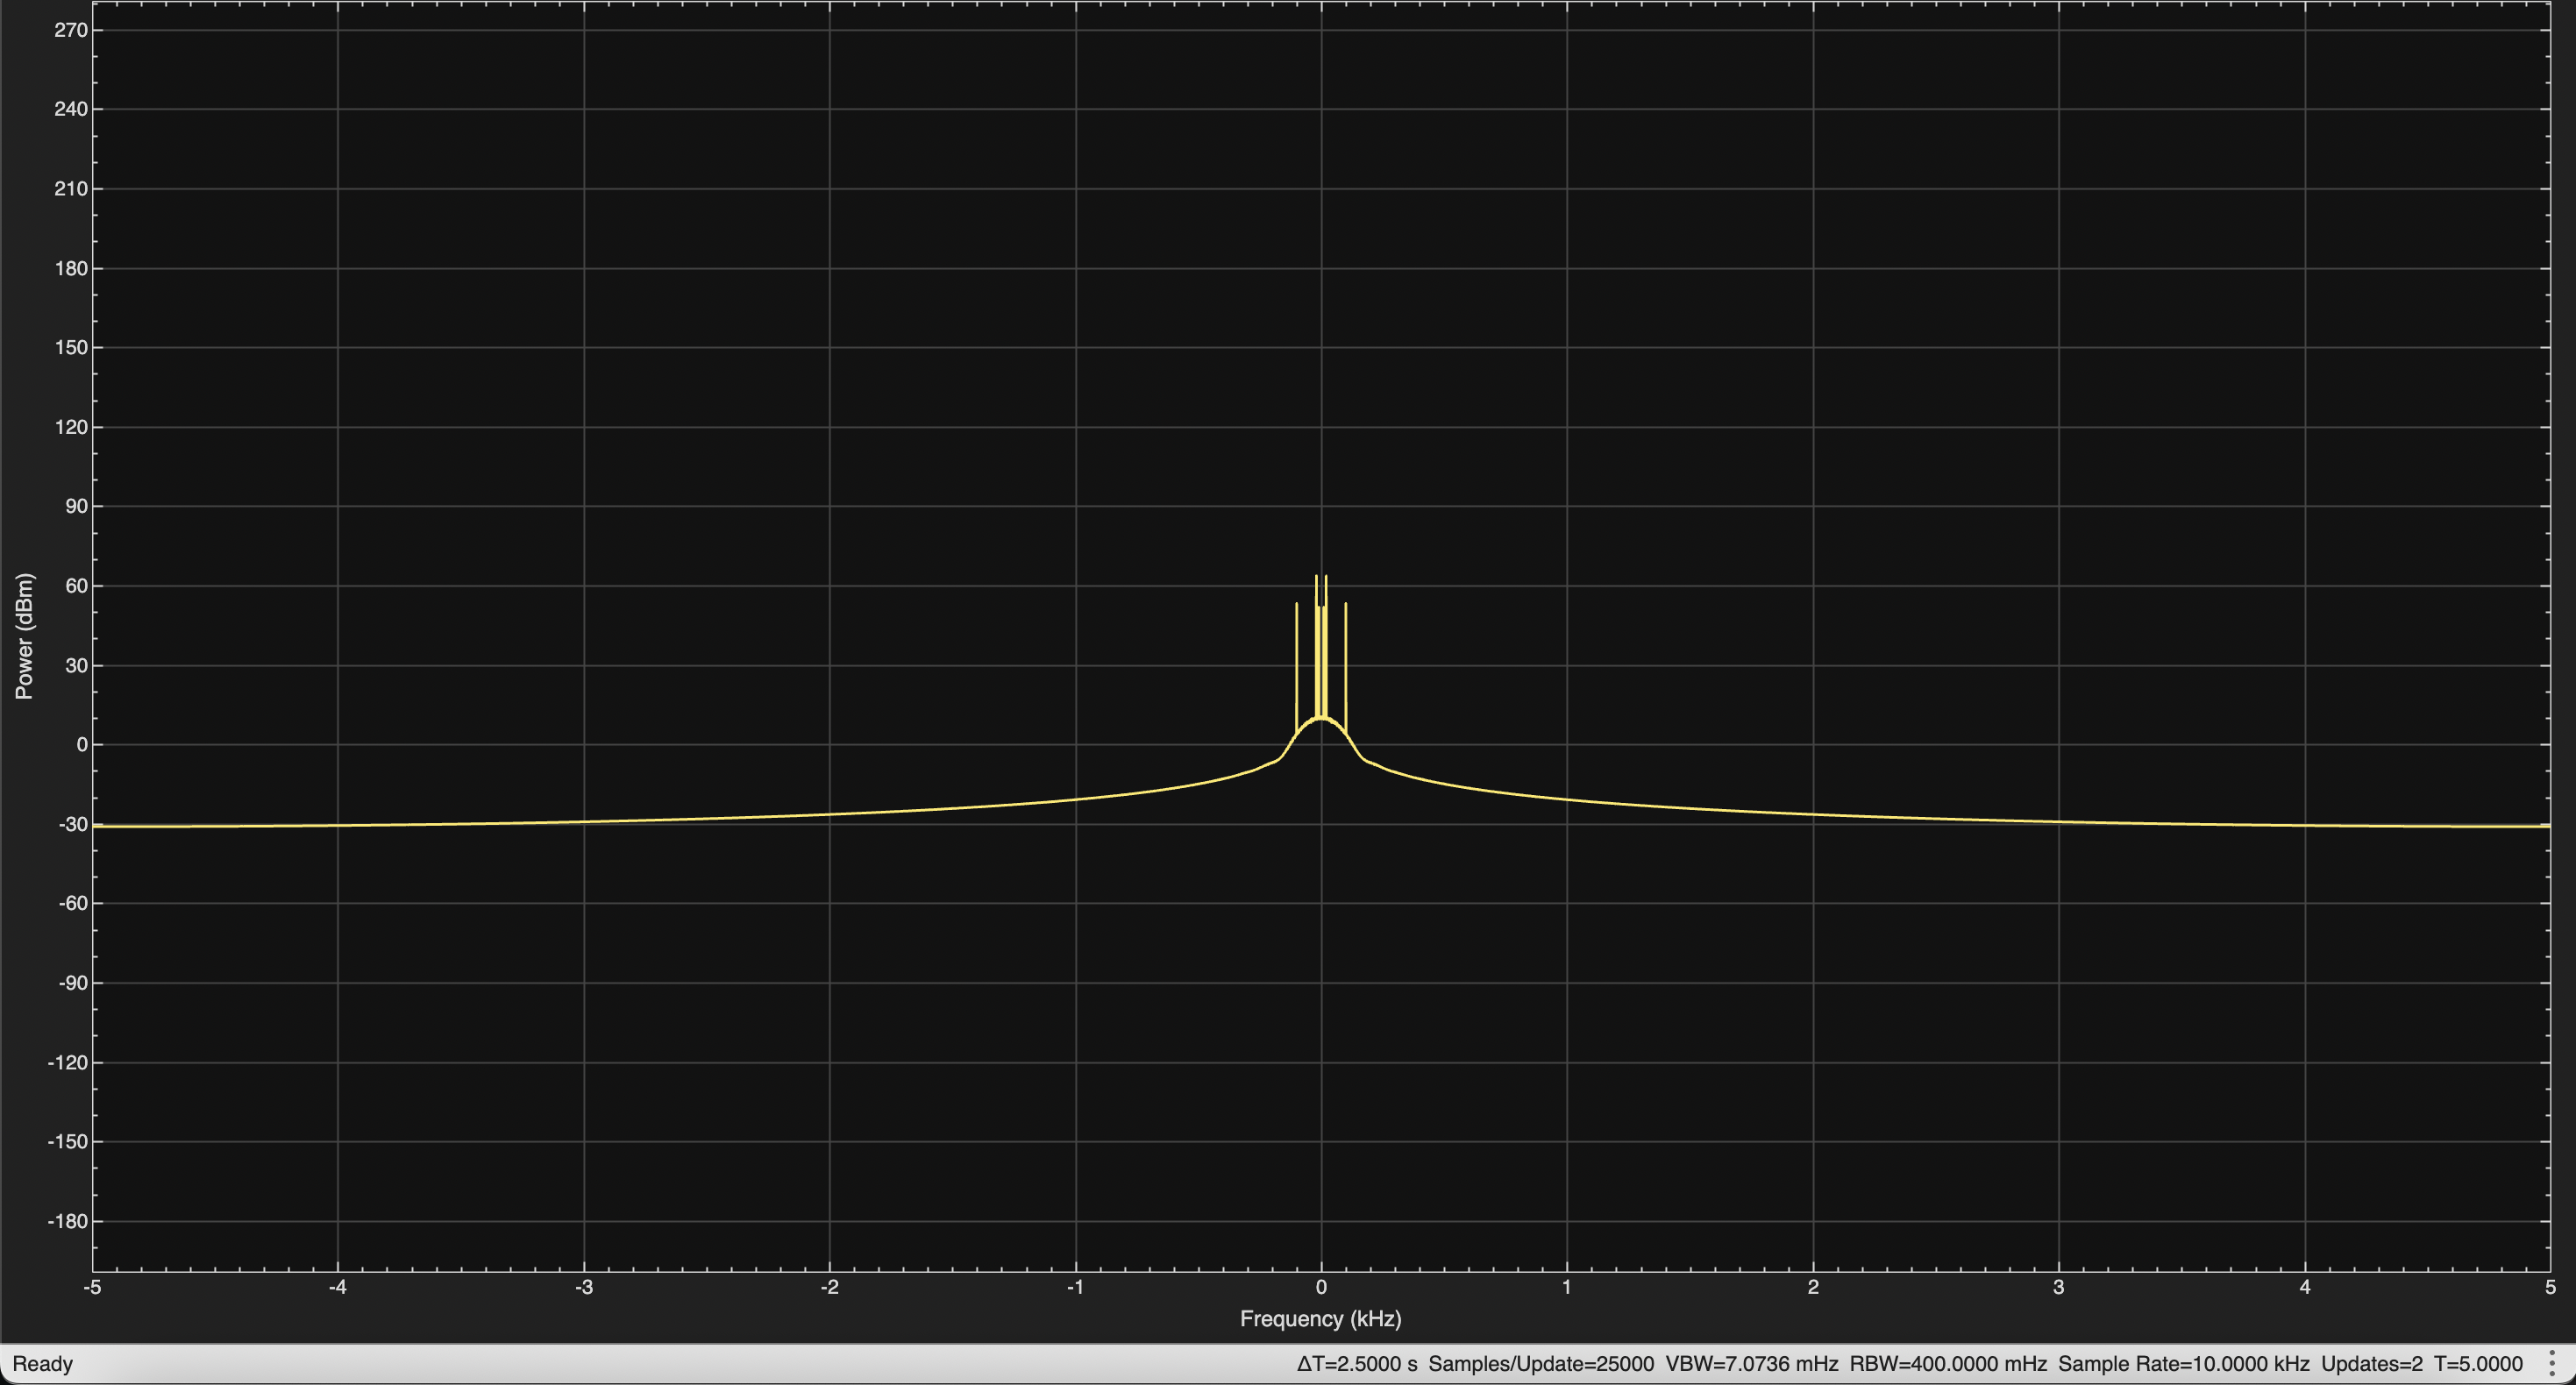
\includegraphics[width=\linewidth]{q2_5_filtered_spectrum_gain_50_fc_100.png}
        \caption{Spectrum.}
    \end{subfigure}
    \caption{Higher gain: filtered sum of three sine waves at gain 50 and $F_c=100$\,Hz.}
    \label{fig:q2-8-gain-50-fc-100}
\end{figure}

\subsubsection*{Varying the cutoff frequency (gain 10)}

\begin{figure}[H]
    \centering
    \begin{subfigure}[b]{0.48\textwidth}
        \centering
        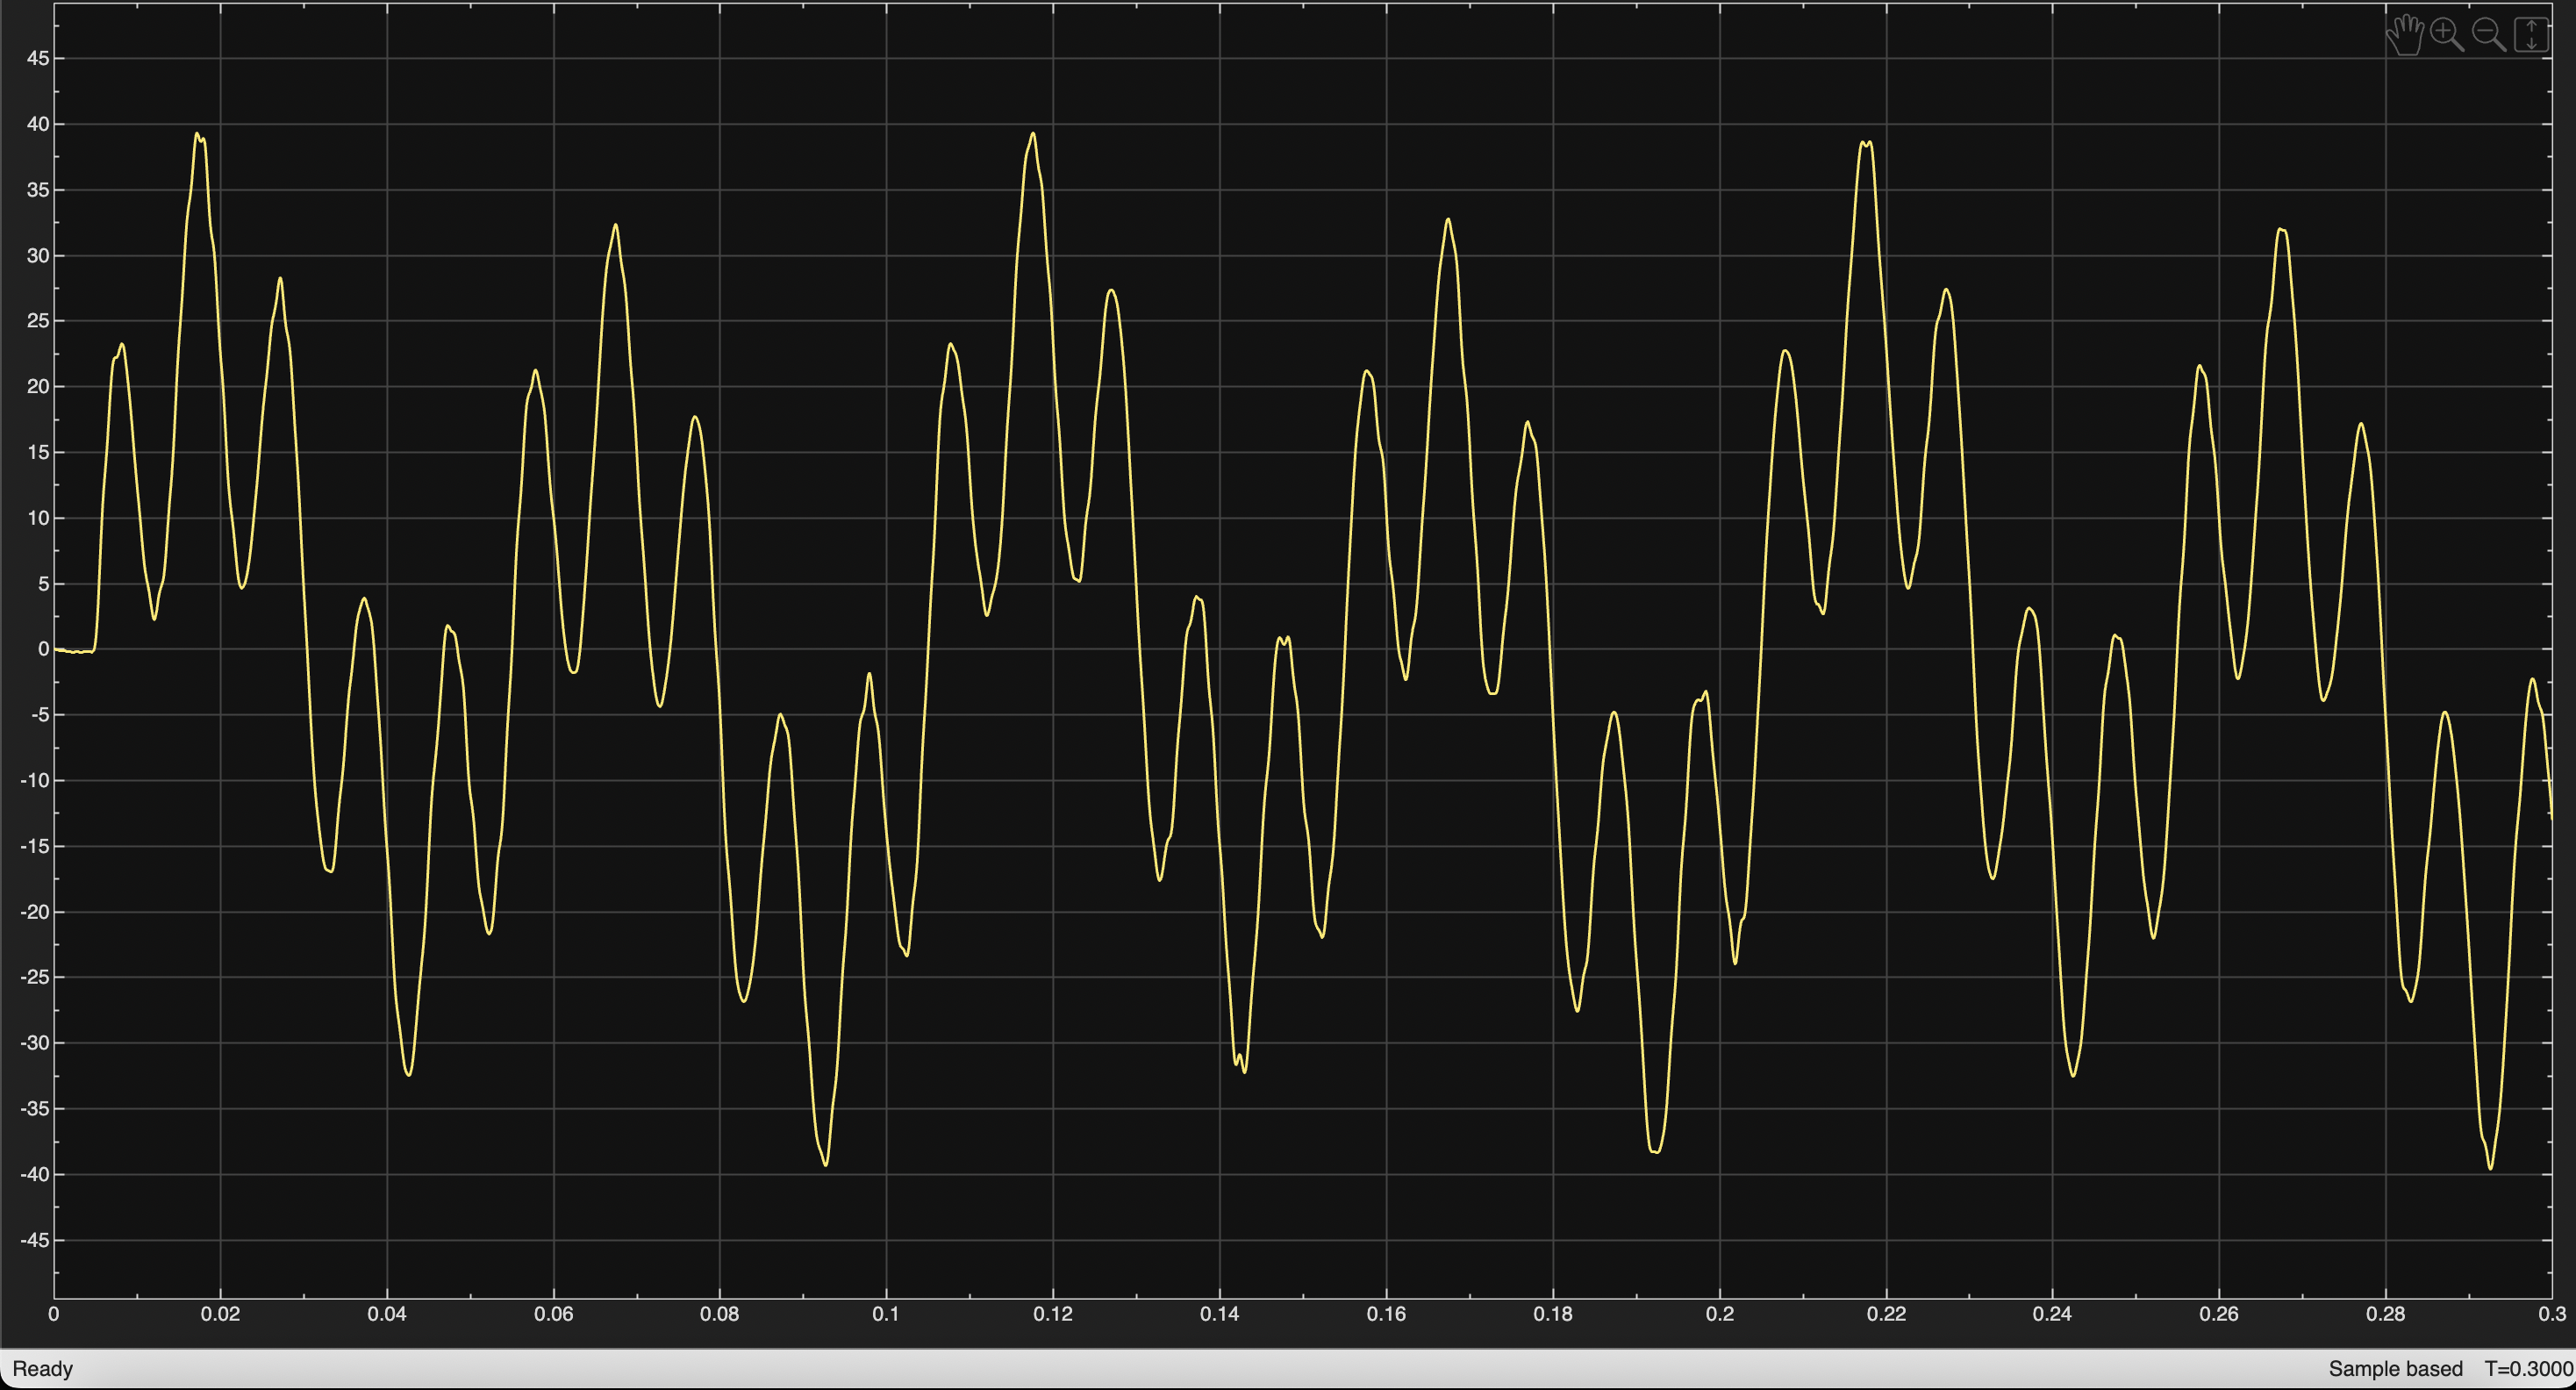
\includegraphics[width=\linewidth]{q2_5_filtered_scope_gain_10_fc_1000.png}
        \caption{Time domain.}
    \end{subfigure}
    \hfill
    \begin{subfigure}[b]{0.48\textwidth}
        \centering
        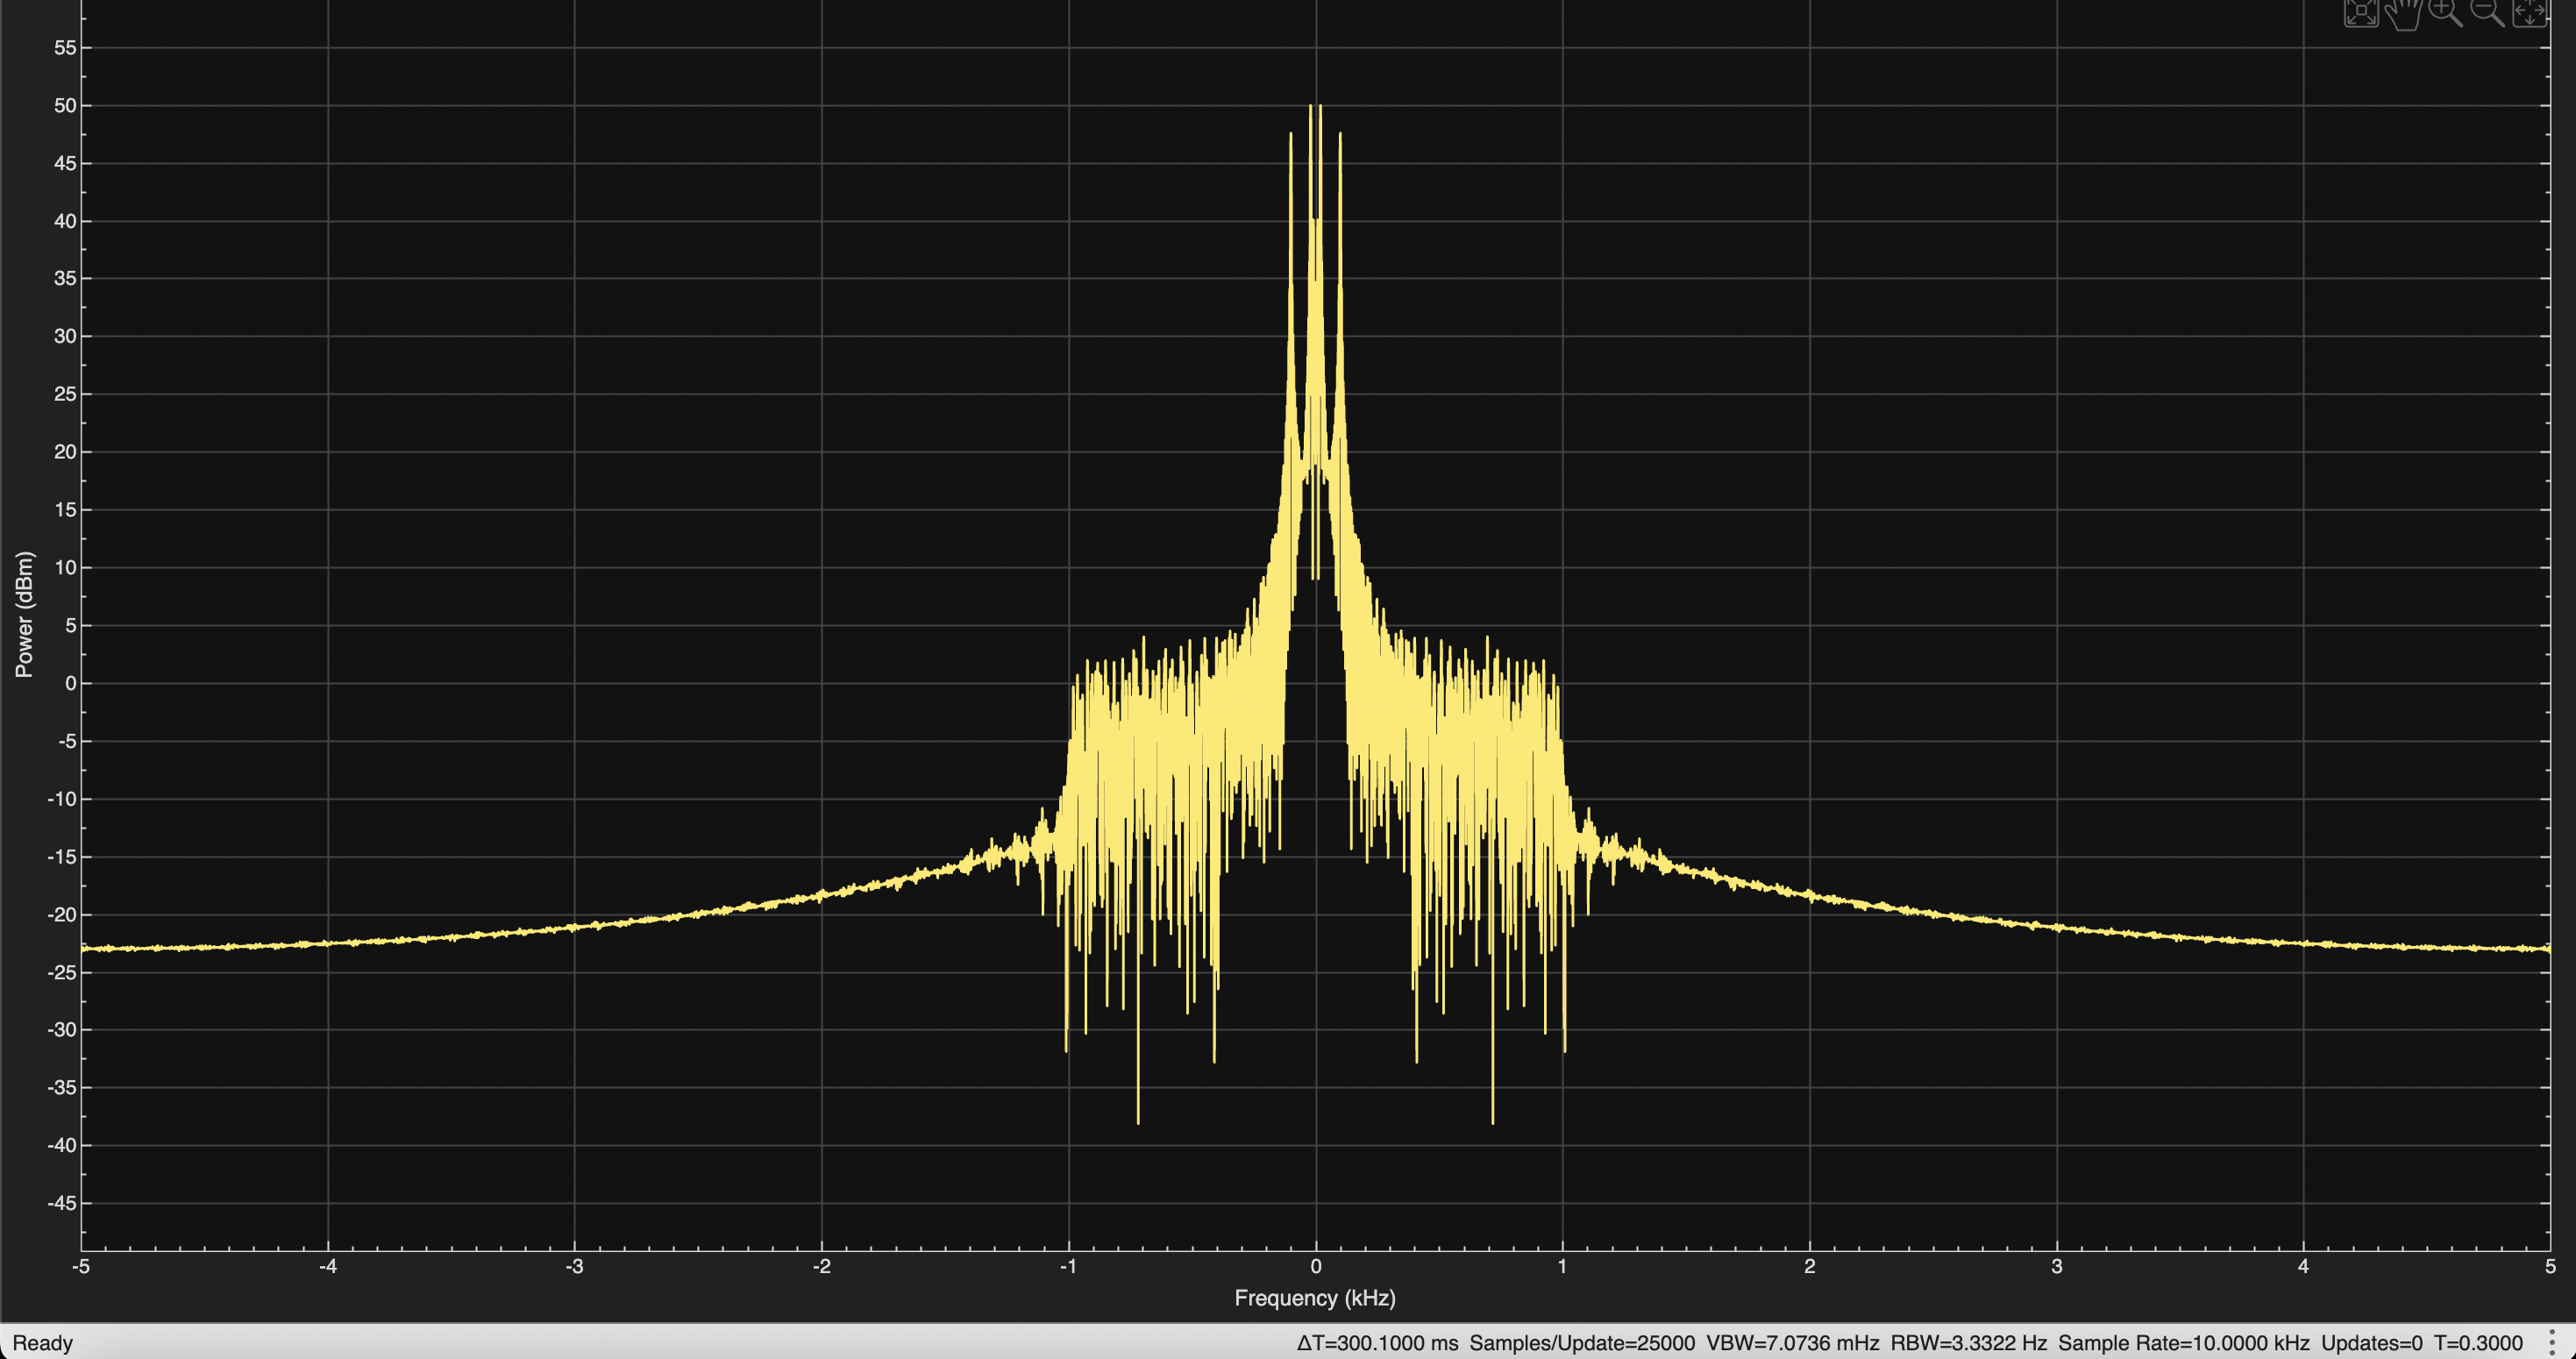
\includegraphics[width=\linewidth]{q2_5_filtered_spectrum_gain_10_fc_1000.png}
        \caption{Spectrum.}
    \end{subfigure}
    \caption{Higher cutoff frequency: filtered sum of three sine waves at gain 10 and $F_c=1000$\,Hz.}
    \label{fig:q2-8-gain-10-fc-1000}
\end{figure}

\begin{figure}[H]
    \centering
    \begin{subfigure}[b]{0.48\textwidth}
        \centering
        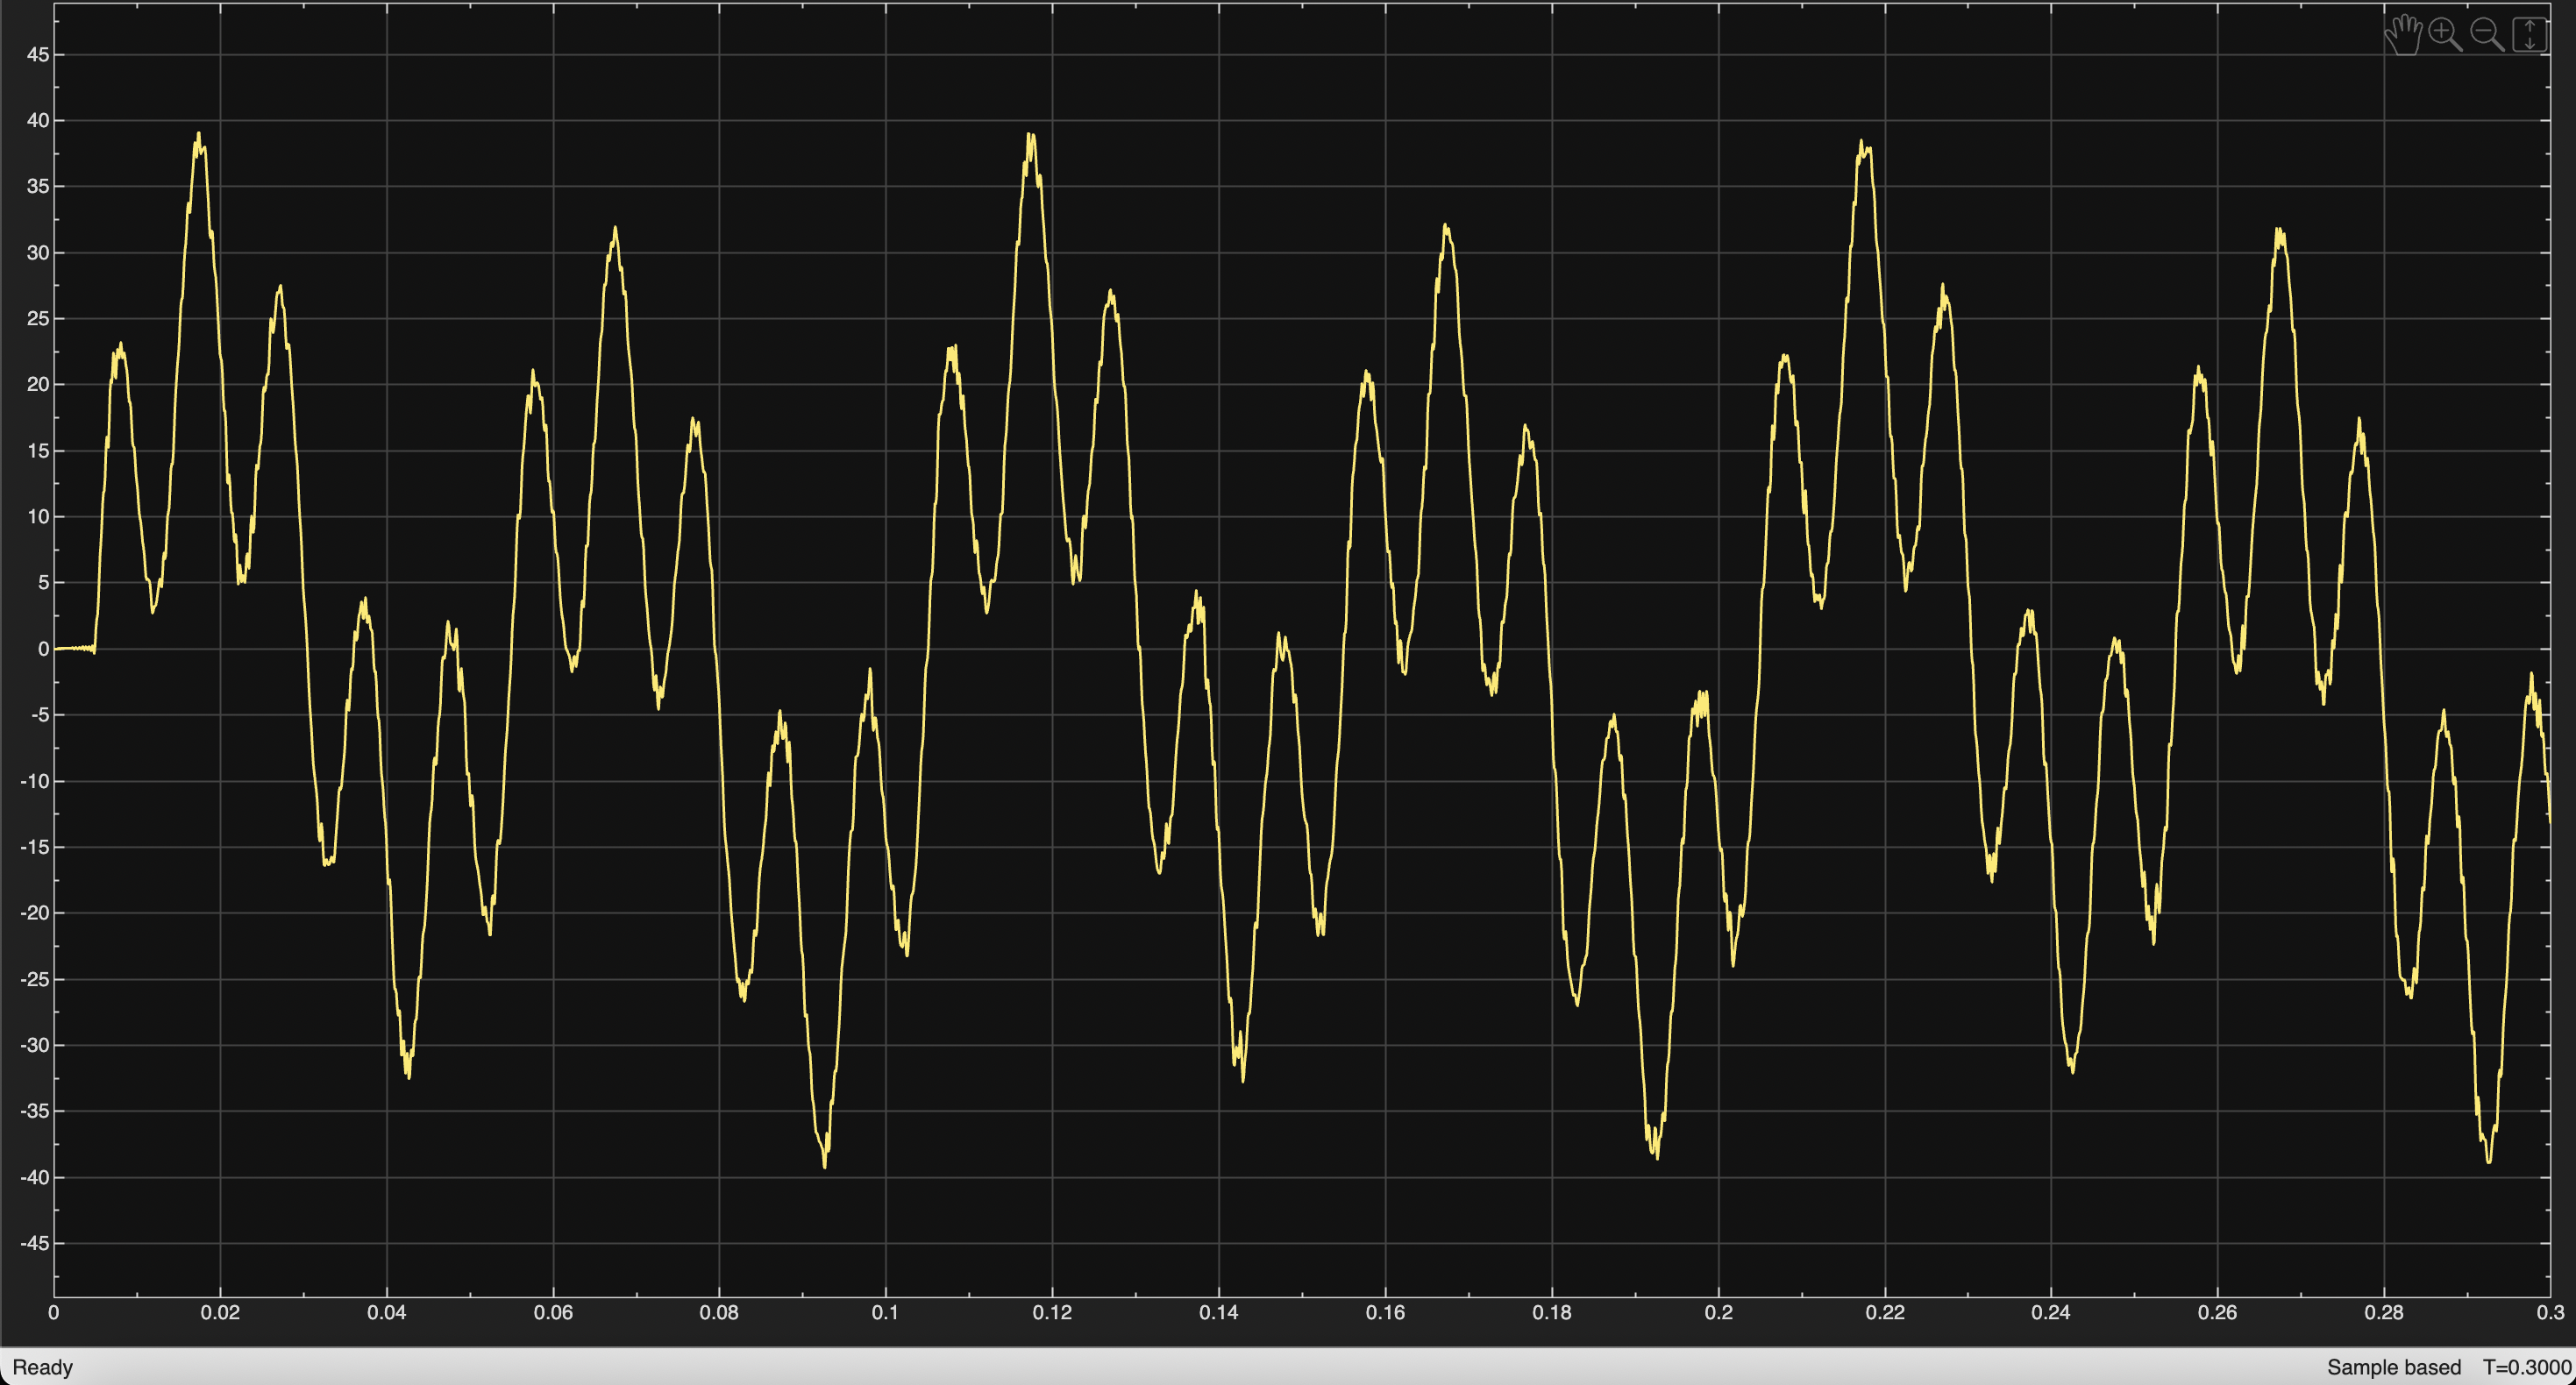
\includegraphics[width=\linewidth]{q2_5_filtered_scope_gain_10_fc_2500.png}
        \caption{Time domain.}
    \end{subfigure}
    \hfill
    \begin{subfigure}[b]{0.48\textwidth}
        \centering
        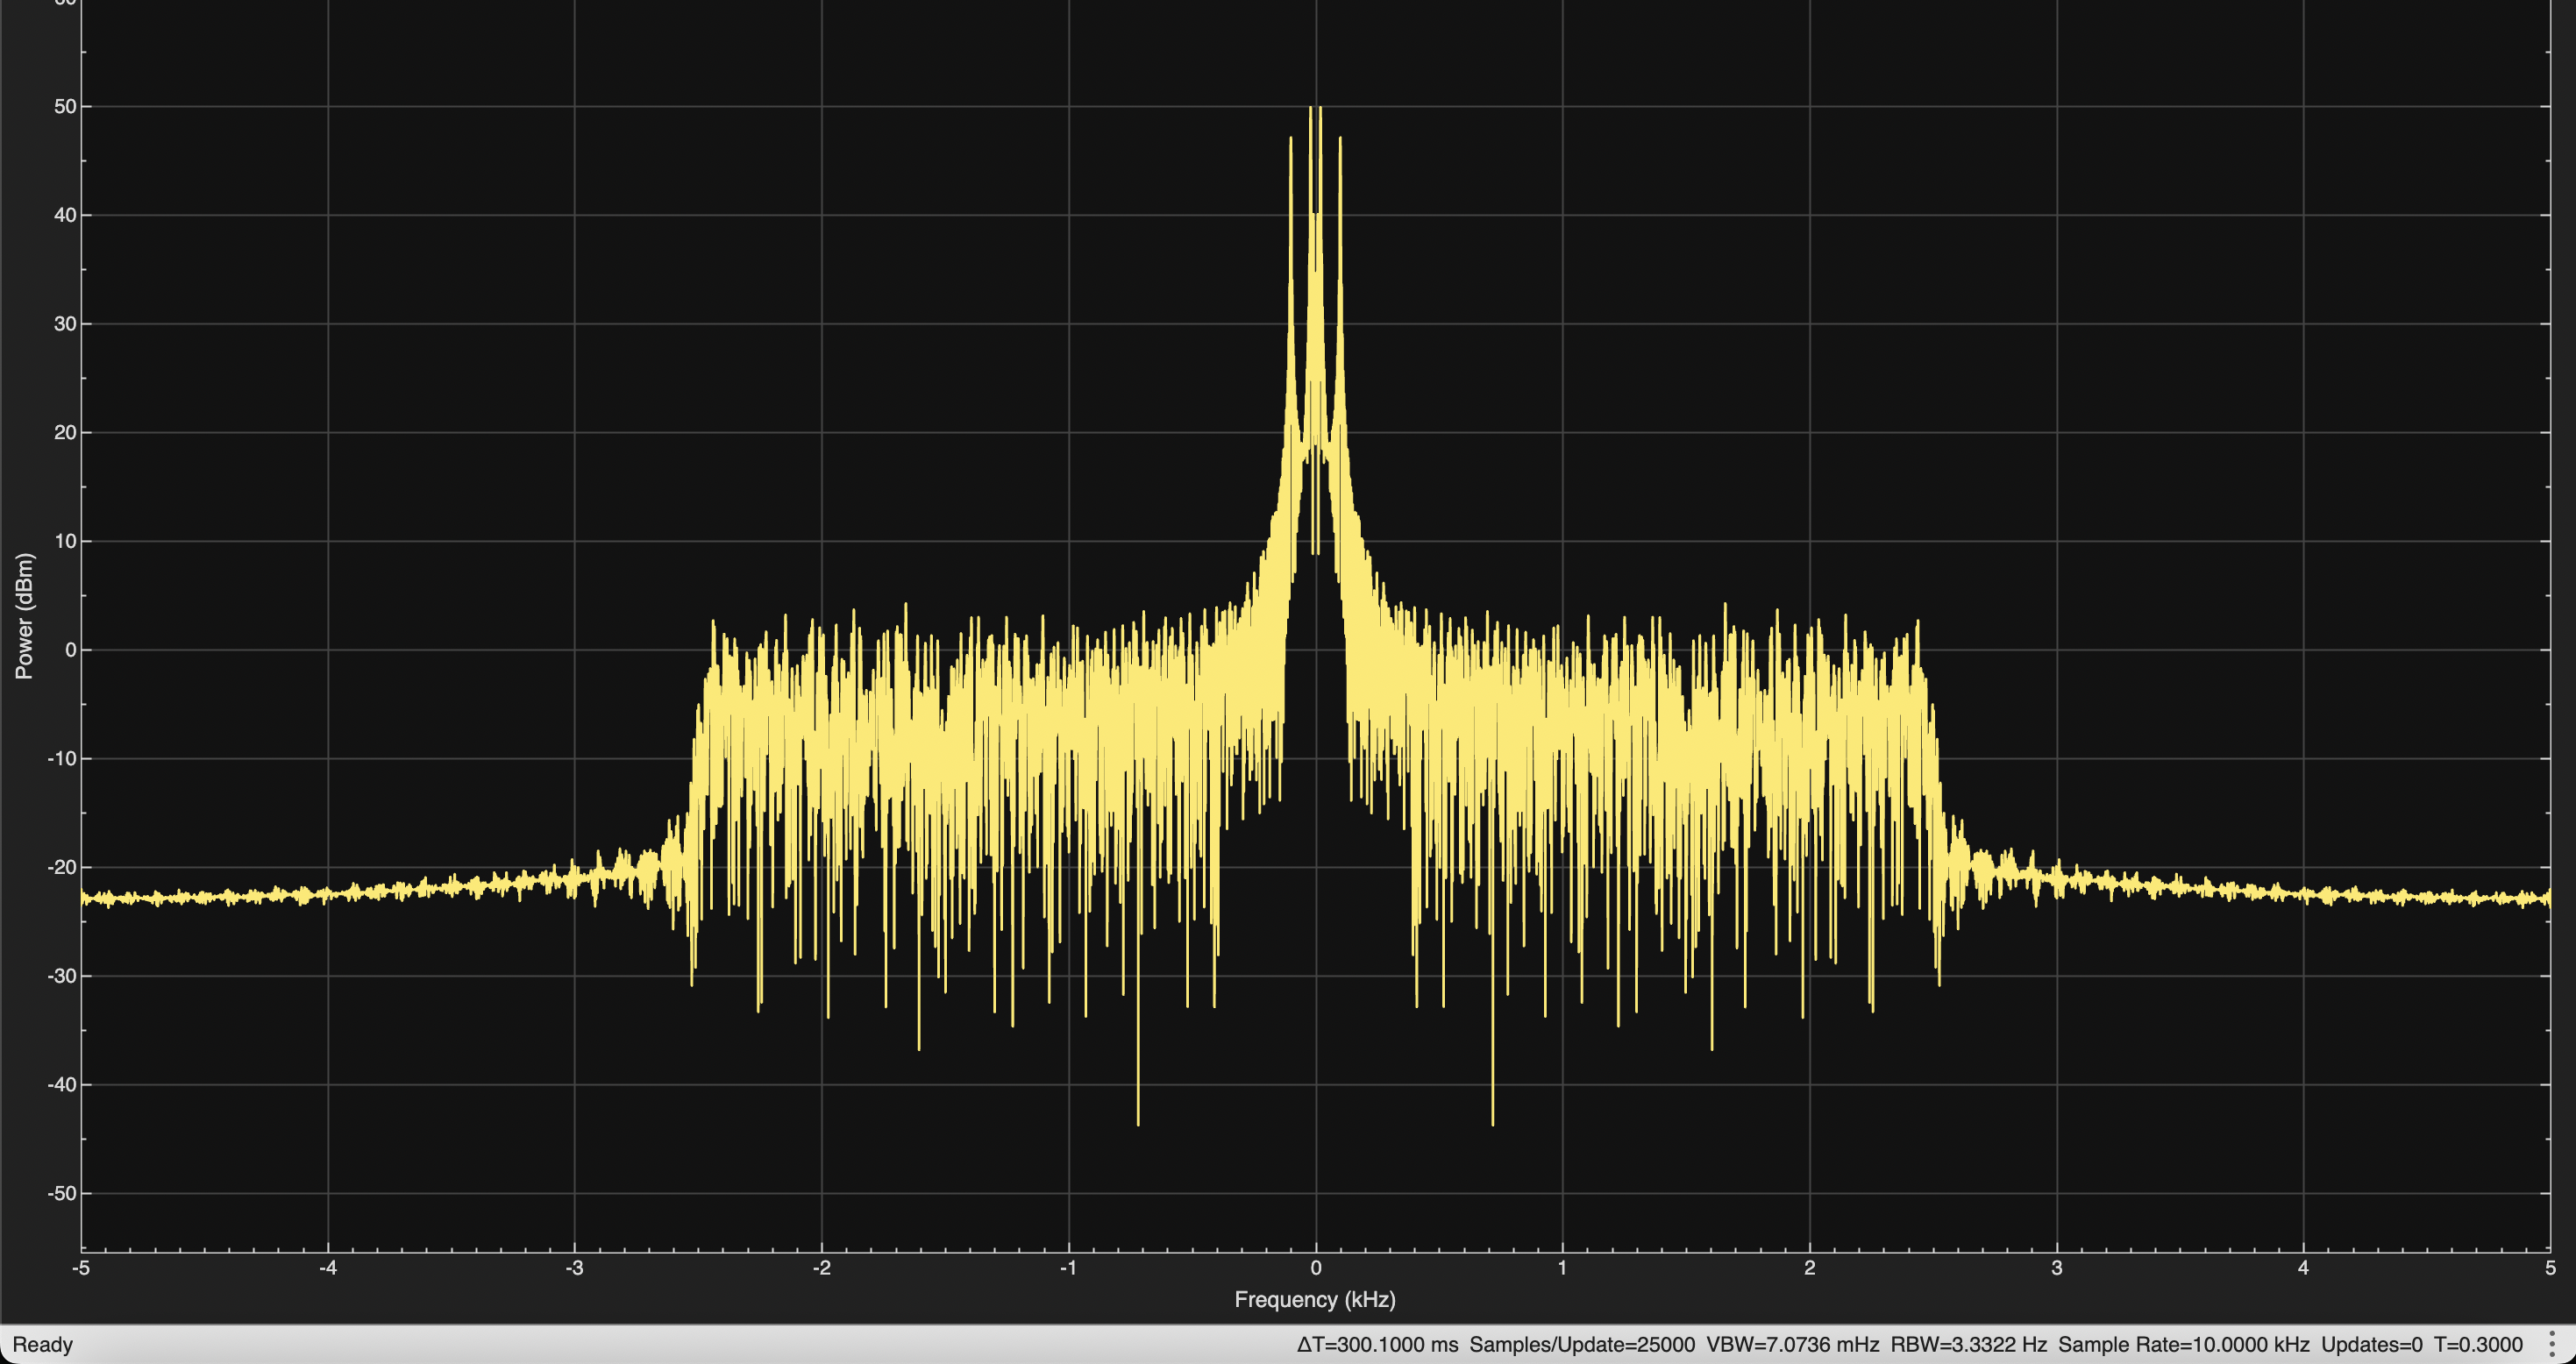
\includegraphics[width=\linewidth]{q2_5_filtered_spectrum_gain_10_fc_2500.png}
        \caption{Spectrum.}
    \end{subfigure}
    \caption{Higher cutoff frequency: filtered sum of three sine waves at gain 10 and $F_c=2500$\,Hz.}
    \label{fig:q2-8-gain-10-fc-2500}
\end{figure}

\end{document}
